\documentclass[twoside]{book}

% Packages required by doxygen
\usepackage{fixltx2e}
\usepackage{calc}
\usepackage{doxygen}
\usepackage[export]{adjustbox} % also loads graphicx
\usepackage{graphicx}
\usepackage[utf8]{inputenc}
\usepackage{makeidx}
\usepackage{multicol}
\usepackage{multirow}
\PassOptionsToPackage{warn}{textcomp}
\usepackage{textcomp}
\usepackage[nointegrals]{wasysym}
\usepackage[table]{xcolor}

% NLS support packages
\usepackage[spanish]{babel}
% Font selection
\usepackage[T1]{fontenc}
\usepackage[scaled=.90]{helvet}
\usepackage{courier}
\usepackage{amssymb}
\usepackage{sectsty}
\renewcommand{\familydefault}{\sfdefault}
\allsectionsfont{%
  \fontseries{bc}\selectfont%
  \color{darkgray}%
}
\renewcommand{\DoxyLabelFont}{%
  \fontseries{bc}\selectfont%
  \color{darkgray}%
}
\newcommand{\+}{\discretionary{\mbox{\scriptsize$\hookleftarrow$}}{}{}}

% Page & text layout
\usepackage{geometry}
\geometry{%
  a4paper,%
  top=2.5cm,%
  bottom=2.5cm,%
  left=2.5cm,%
  right=2.5cm%
}
\tolerance=750
\hfuzz=15pt
\hbadness=750
\setlength{\emergencystretch}{15pt}
\setlength{\parindent}{0cm}
\setlength{\parskip}{3ex plus 2ex minus 2ex}
\makeatletter
\renewcommand{\paragraph}{%
  \@startsection{paragraph}{4}{0ex}{-1.0ex}{1.0ex}{%
    \normalfont\normalsize\bfseries\SS@parafont%
  }%
}
\renewcommand{\subparagraph}{%
  \@startsection{subparagraph}{5}{0ex}{-1.0ex}{1.0ex}{%
    \normalfont\normalsize\bfseries\SS@subparafont%
  }%
}
\makeatother

% Headers & footers
\usepackage{fancyhdr}
\pagestyle{fancyplain}
\fancyhead[LE]{\fancyplain{}{\bfseries\thepage}}
\fancyhead[CE]{\fancyplain{}{}}
\fancyhead[RE]{\fancyplain{}{\bfseries\leftmark}}
\fancyhead[LO]{\fancyplain{}{\bfseries\rightmark}}
\fancyhead[CO]{\fancyplain{}{}}
\fancyhead[RO]{\fancyplain{}{\bfseries\thepage}}
\fancyfoot[LE]{\fancyplain{}{}}
\fancyfoot[CE]{\fancyplain{}{}}
\fancyfoot[RE]{\fancyplain{}{\bfseries\scriptsize Generado por Doxygen }}
\fancyfoot[LO]{\fancyplain{}{\bfseries\scriptsize Generado por Doxygen }}
\fancyfoot[CO]{\fancyplain{}{}}
\fancyfoot[RO]{\fancyplain{}{}}
\renewcommand{\footrulewidth}{0.4pt}
\renewcommand{\chaptermark}[1]{%
  \markboth{#1}{}%
}
\renewcommand{\sectionmark}[1]{%
  \markright{\thesection\ #1}%
}

% Indices & bibliography
\usepackage{natbib}
\usepackage[titles]{tocloft}
\setcounter{tocdepth}{3}
\setcounter{secnumdepth}{5}
\makeindex

% Hyperlinks (required, but should be loaded last)
\usepackage{ifpdf}
\ifpdf
  \usepackage[pdftex,pagebackref=true]{hyperref}
\else
  \usepackage[ps2pdf,pagebackref=true]{hyperref}
\fi
\hypersetup{%
  colorlinks=true,%
  linkcolor=blue,%
  citecolor=blue,%
  unicode%
}

% Custom commands
\newcommand{\clearemptydoublepage}{%
  \newpage{\pagestyle{empty}\cleardoublepage}%
}

\usepackage{caption}
\captionsetup{labelsep=space,justification=centering,font={bf},singlelinecheck=off,skip=4pt,position=top}

%===== C O N T E N T S =====

\begin{document}

% Titlepage & ToC
\hypersetup{pageanchor=false,
             bookmarksnumbered=true,
             pdfencoding=unicode
            }
\pagenumbering{alph}
\begin{titlepage}
\vspace*{7cm}
\begin{center}%
{\Large Libreria L\+P\+C845 }\\
\vspace*{1cm}
{\large Generado por Doxygen 1.8.13}\\
\end{center}
\end{titlepage}
\clearemptydoublepage
\pagenumbering{roman}
\tableofcontents
\clearemptydoublepage
\pagenumbering{arabic}
\hypersetup{pageanchor=true}

%--- Begin generated contents ---
\chapter{Pagina principal de la documentacion}
\label{index}\hypertarget{index}{}\hypertarget{index_intro}{}\section{Introduccion}\label{index_intro}
Esta libreria esta pensada para... (bla bla bla)

Mañana mismo me pongo a escribir esto! 
\chapter{Indice de módulos}
\doxysection{Módulos}
Lista de todos los módulos\+:\begin{DoxyCompactList}
\item \contentsline{section}{Conversor analógico a digital (A\+DC)}{\pageref{group__ADC}}{}
\end{DoxyCompactList}

\chapter{Índice de estructura de datos}
\section{Estructura de datos}
Lista de estructuras con una breve descripción\+:\begin{DoxyCompactList}
\item\contentsline{section}{\hyperlink{structCTIMER__CC__config__t}{C\+T\+I\+M\+E\+R\+\_\+\+C\+C\+\_\+config\+\_\+t} }{\pageref{structCTIMER__CC__config__t}}{}
\item\contentsline{section}{\hyperlink{structCTIMER__MR__config__t}{C\+T\+I\+M\+E\+R\+\_\+\+M\+R\+\_\+config\+\_\+t} }{\pageref{structCTIMER__MR__config__t}}{}
\item\contentsline{section}{\hyperlink{structhal__adc__sequence__config__t}{hal\+\_\+adc\+\_\+sequence\+\_\+config\+\_\+t} }{\pageref{structhal__adc__sequence__config__t}}{}
\item\contentsline{section}{\hyperlink{structhal__ctimer__match__config__t}{hal\+\_\+ctimer\+\_\+match\+\_\+config\+\_\+t} }{\pageref{structhal__ctimer__match__config__t}}{}
\item\contentsline{section}{\hyperlink{structhal__ctimer__pwm__channel__config__t}{hal\+\_\+ctimer\+\_\+pwm\+\_\+channel\+\_\+config\+\_\+t} }{\pageref{structhal__ctimer__pwm__channel__config__t}}{}
\item\contentsline{section}{\hyperlink{structhal__ctimer__pwm__config__t}{hal\+\_\+ctimer\+\_\+pwm\+\_\+config\+\_\+t} }{\pageref{structhal__ctimer__pwm__config__t}}{}
\item\contentsline{section}{\hyperlink{structhal__pinint__config__t}{hal\+\_\+pinint\+\_\+config\+\_\+t} }{\pageref{structhal__pinint__config__t}}{}
\item\contentsline{section}{\hyperlink{structhal__spi__master__mode__config__t}{hal\+\_\+spi\+\_\+master\+\_\+mode\+\_\+config\+\_\+t} }{\pageref{structhal__spi__master__mode__config__t}}{}
\item\contentsline{section}{\hyperlink{structhal__uart__config__t}{hal\+\_\+uart\+\_\+config\+\_\+t} }{\pageref{structhal__uart__config__t}}{}
\item\contentsline{section}{\hyperlink{structIOCON__per__t}{I\+O\+C\+O\+N\+\_\+per\+\_\+t} }{\pageref{structIOCON__per__t}}{}
\item\contentsline{section}{\hyperlink{structIOCON__PIO__reg__t}{I\+O\+C\+O\+N\+\_\+\+P\+I\+O\+\_\+reg\+\_\+t} }{\pageref{structIOCON__PIO__reg__t}}{}
\item\contentsline{section}{\hyperlink{structtimer__t}{timer\+\_\+t} }{\pageref{structtimer__t}}{}
\end{DoxyCompactList}

\chapter{Indice de archivos}
\section{Lista de archivos}
Lista de todos los archivos documentados y con descripciones breves\+:\begin{DoxyCompactList}
\item\contentsline{section}{includes/hal/\hyperlink{HAL__ADC_8h}{H\+A\+L\+\_\+\+A\+D\+C.\+h} \\*Declaraciones a nivel de aplicacion del periferico A\+DC (L\+P\+C845) }{\pageref{HAL__ADC_8h}}{}
\item\contentsline{section}{includes/hal/\hyperlink{HAL__CTIMER_8h}{H\+A\+L\+\_\+\+C\+T\+I\+M\+E\+R.\+h} \\*Declaraciones a nivel de aplicacion del periferico C\+T\+I\+M\+ER (L\+P\+C845) }{\pageref{HAL__CTIMER_8h}}{}
\item\contentsline{section}{includes/hal/\hyperlink{HAL__DAC_8h}{H\+A\+L\+\_\+\+D\+A\+C.\+h} \\*Declaraciones a nivel de aplicacion del periferico D\+AC (L\+P\+C845) }{\pageref{HAL__DAC_8h}}{}
\item\contentsline{section}{includes/hal/\hyperlink{HAL__GPIO_8h}{H\+A\+L\+\_\+\+G\+P\+I\+O.\+h} \\*Declaraciones a nivel de aplicacion del periferico G\+P\+IO (L\+P\+C845) }{\pageref{HAL__GPIO_8h}}{}
\item\contentsline{section}{includes/hal/\hyperlink{HAL__IOCON_8h}{H\+A\+L\+\_\+\+I\+O\+C\+O\+N.\+h} \\*Declaraciones a nivel de aplicacion del periferico I\+O\+C\+ON (L\+P\+C845) }{\pageref{HAL__IOCON_8h}}{}
\item\contentsline{section}{includes/hal/\hyperlink{HAL__PININT_8h}{H\+A\+L\+\_\+\+P\+I\+N\+I\+N\+T.\+h} \\*Declaraciones a nivel de aplicacion del periferico P\+I\+N\+I\+NT (L\+P\+C845) }{\pageref{HAL__PININT_8h}}{}
\item\contentsline{section}{includes/hal/\hyperlink{HAL__SPI_8h}{H\+A\+L\+\_\+\+S\+P\+I.\+h} \\*Declaraciones a nivel de aplicacion del periferico S\+PI (L\+P\+C845) }{\pageref{HAL__SPI_8h}}{}
\item\contentsline{section}{includes/hal/\hyperlink{HAL__SYSCON_8h}{H\+A\+L\+\_\+\+S\+Y\+S\+C\+O\+N.\+h} \\*Declaraciones a nivel de aplicacion del periferico S\+Y\+S\+C\+ON (L\+P\+C845) }{\pageref{HAL__SYSCON_8h}}{}
\item\contentsline{section}{includes/hal/\hyperlink{HAL__SYSTICK_8h}{H\+A\+L\+\_\+\+S\+Y\+S\+T\+I\+C\+K.\+h} \\*Declaraciones a nivel de aplicacion del periferico S\+Y\+S\+I\+CK (L\+P\+C845) }{\pageref{HAL__SYSTICK_8h}}{}
\item\contentsline{section}{includes/hal/\hyperlink{HAL__UART_8h}{H\+A\+L\+\_\+\+U\+A\+R\+T.\+h} \\*Declaraciones a nivel de aplicacion del periferico U\+A\+RT (L\+P\+C845) }{\pageref{HAL__UART_8h}}{}
\item\contentsline{section}{includes/hal/\hyperlink{HAL__WKT_8h}{H\+A\+L\+\_\+\+W\+K\+T.\+h} \\*Declaraciones a nivel de aplicacion del periferico W\+KT (L\+P\+C845) }{\pageref{HAL__WKT_8h}}{}
\item\contentsline{section}{includes/hpl/\hyperlink{HPL__ADC_8h}{H\+P\+L\+\_\+\+A\+D\+C.\+h} \\*Declaraciones a nivel de abstraccion de periferico del A\+DC (L\+P\+C845) }{\pageref{HPL__ADC_8h}}{}
\item\contentsline{section}{includes/hpl/\hyperlink{HPL__CTIMER_8h}{H\+P\+L\+\_\+\+C\+T\+I\+M\+E\+R.\+h} \\*Definiciones a nivel de abstraccion del periferico C\+T\+I\+M\+ER (L\+P\+C845) }{\pageref{HPL__CTIMER_8h}}{}
\item\contentsline{section}{includes/hpl/\hyperlink{HPL__DAC_8h}{H\+P\+L\+\_\+\+D\+A\+C.\+h} \\*Declaraciones a nivel de abstraccion de periferico del D\+AC (L\+P\+C845) }{\pageref{HPL__DAC_8h}}{}
\item\contentsline{section}{includes/hpl/\hyperlink{HPL__GPIO_8h}{H\+P\+L\+\_\+\+G\+P\+I\+O.\+h} \\*Declaraciones a nivel de abstraccion de periferico del G\+P\+IO (L\+P\+C845) }{\pageref{HPL__GPIO_8h}}{}
\item\contentsline{section}{includes/hpl/\hyperlink{HPL__IOCON_8h}{H\+P\+L\+\_\+\+I\+O\+C\+O\+N.\+h} \\*Declaraciones a nivel de abstraccion de periferico del I\+O\+C\+ON (L\+P\+C845) }{\pageref{HPL__IOCON_8h}}{}
\item\contentsline{section}{includes/hpl/\hyperlink{HPL__MRT_8h}{H\+P\+L\+\_\+\+M\+R\+T.\+h} \\*Declaraciones a nivel de abstraccion de periferico del M\+RT (L\+P\+C845) }{\pageref{HPL__MRT_8h}}{}
\item\contentsline{section}{includes/hpl/\hyperlink{HPL__NVIC_8h}{H\+P\+L\+\_\+\+N\+V\+I\+C.\+h} \\*Declaraciones a nivel de abstraccion de periferico del N\+V\+IC (L\+P\+C845) }{\pageref{HPL__NVIC_8h}}{}
\item\contentsline{section}{includes/hpl/\hyperlink{HPL__PININT_8h}{H\+P\+L\+\_\+\+P\+I\+N\+I\+N\+T.\+h} \\*Declaraciones a nivel de abstraccion de periferico del P\+I\+N\+I\+NT (L\+P\+C845) }{\pageref{HPL__PININT_8h}}{}
\item\contentsline{section}{includes/hpl/\hyperlink{HPL__PMU_8h}{H\+P\+L\+\_\+\+P\+M\+U.\+h} \\*Declaraciones a nivel de abstraccion de periferico del P\+MU (L\+P\+C845) }{\pageref{HPL__PMU_8h}}{}
\item\contentsline{section}{includes/hpl/\hyperlink{HPL__SPI_8h}{H\+P\+L\+\_\+\+S\+P\+I.\+h} \\*Declaraciones a nivel de abstraccion de periferico del S\+PI (L\+P\+C845) }{\pageref{HPL__SPI_8h}}{}
\item\contentsline{section}{includes/hpl/\hyperlink{HPL__SWM_8h}{H\+P\+L\+\_\+\+S\+W\+M.\+h} \\*Definiciones a nivel de periferico del modulo S\+WM (L\+P\+C845) }{\pageref{HPL__SWM_8h}}{}
\item\contentsline{section}{includes/hpl/\hyperlink{HPL__SYSCON_8h}{H\+P\+L\+\_\+\+S\+Y\+S\+C\+O\+N.\+h} \\*Declaraciones a nivel de abstraccion de periferico del S\+Y\+S\+C\+ON (L\+P\+C845) }{\pageref{HPL__SYSCON_8h}}{}
\item\contentsline{section}{includes/hpl/\hyperlink{HPL__SYSTICK_8h}{H\+P\+L\+\_\+\+S\+Y\+S\+T\+I\+C\+K.\+h} \\*Declaraciones a nivel de abstraccion de periferico del S\+Y\+S\+T\+I\+CK (L\+P\+C845) }{\pageref{HPL__SYSTICK_8h}}{}
\item\contentsline{section}{includes/hpl/\hyperlink{HPL__UART_8h}{H\+P\+L\+\_\+\+U\+A\+R\+T.\+h} \\*Declaraciones a nivel de abstraccion de periferico del U\+A\+RT (L\+P\+C845) }{\pageref{HPL__UART_8h}}{}
\item\contentsline{section}{includes/hpl/\hyperlink{HPL__WKT_8h}{H\+P\+L\+\_\+\+W\+K\+T.\+h} \\*Declaraciones a nivel de abstraccion de periferico del W\+KT (L\+P\+C845) }{\pageref{HPL__WKT_8h}}{}
\item\contentsline{section}{includes/hri/\hyperlink{HRI__ADC_8h}{H\+R\+I\+\_\+\+A\+D\+C.\+h} \\*Declaraciones a nivel de registros del A\+DC (L\+P\+C845) }{\pageref{HRI__ADC_8h}}{}
\item\contentsline{section}{includes/hri/\hyperlink{HRI__CTIMER_8h}{H\+R\+I\+\_\+\+C\+T\+I\+M\+E\+R.\+h} \\*Definiciones a nivel de registros del periferico C\+T\+I\+M\+ER (L\+P\+C845) }{\pageref{HRI__CTIMER_8h}}{}
\item\contentsline{section}{includes/hri/\hyperlink{HRI__DAC_8h}{H\+R\+I\+\_\+\+D\+A\+C.\+h} \\*Declaraciones a nivel de registros del D\+AC (L\+P\+C845) }{\pageref{HRI__DAC_8h}}{}
\item\contentsline{section}{includes/hri/\hyperlink{HRI__GPIO_8h}{H\+R\+I\+\_\+\+G\+P\+I\+O.\+h} \\*Definiciones a nivel de registros del modulo G\+P\+IO (L\+P\+C845) }{\pageref{HRI__GPIO_8h}}{}
\item\contentsline{section}{includes/hri/{\bfseries H\+R\+I\+\_\+\+I\+O\+C\+O\+N.\+h} }{\pageref{HRI__IOCON_8h}}{}
\item\contentsline{section}{includes/hri/\hyperlink{HRI__MRT_8h}{H\+R\+I\+\_\+\+M\+R\+T.\+h} \\*Definiciones a nivel de registros del periferico M\+RT (L\+P\+C845) }{\pageref{HRI__MRT_8h}}{}
\item\contentsline{section}{includes/hri/\hyperlink{HRI__NVIC_8h}{H\+R\+I\+\_\+\+N\+V\+I\+C.\+h} \\*Definiciones a nivel de registros del modulo N\+V\+IC (L\+P\+C845) }{\pageref{HRI__NVIC_8h}}{}
\item\contentsline{section}{includes/hri/\hyperlink{HRI__PININT_8h}{H\+R\+I\+\_\+\+P\+I\+N\+I\+N\+T.\+h} \\*Definiciones a nivel de registros del modulo P\+I\+N\+I\+NT (L\+P\+C845) }{\pageref{HRI__PININT_8h}}{}
\item\contentsline{section}{includes/hri/\hyperlink{HRI__PMU_8h}{H\+R\+I\+\_\+\+P\+M\+U.\+h} \\*Definiciones a nivel de registros del modulo P\+MU (L\+P\+C845) }{\pageref{HRI__PMU_8h}}{}
\item\contentsline{section}{includes/hri/\hyperlink{HRI__SPI_8h}{H\+R\+I\+\_\+\+S\+P\+I.\+h} \\*Definiciones a nivel de registros del periferico S\+PI (L\+P\+C845) }{\pageref{HRI__SPI_8h}}{}
\item\contentsline{section}{includes/hri/\hyperlink{HRI__SWM_8h}{H\+R\+I\+\_\+\+S\+W\+M.\+h} \\*Definiciones a nivel de registros del modulo S\+WM (L\+P\+C845) }{\pageref{HRI__SWM_8h}}{}
\item\contentsline{section}{includes/hri/\hyperlink{HRI__SYSCON_8h}{H\+R\+I\+\_\+\+S\+Y\+S\+C\+O\+N.\+h} \\*Definiciones a nivel de registros del modulo S\+Y\+S\+C\+ON (L\+P\+C845) }{\pageref{HRI__SYSCON_8h}}{}
\item\contentsline{section}{includes/hri/\hyperlink{HRI__SYSTICK_8h}{H\+R\+I\+\_\+\+S\+Y\+S\+T\+I\+C\+K.\+h} \\*Definiciones a nivel de registros del modulo S\+Y\+S\+T\+I\+CK (L\+P\+C845) }{\pageref{HRI__SYSTICK_8h}}{}
\item\contentsline{section}{includes/hri/\hyperlink{HRI__UART_8h}{H\+R\+I\+\_\+\+U\+A\+R\+T.\+h} \\*Definiciones a nivel de registros del modulo U\+A\+RT (L\+P\+C845) }{\pageref{HRI__UART_8h}}{}
\item\contentsline{section}{includes/hri/\hyperlink{HRI__WKT_8h}{H\+R\+I\+\_\+\+W\+K\+T.\+h} \\*Definiciones a nivel de registros del periferico W\+KT (L\+P\+C845) }{\pageref{HRI__WKT_8h}}{}
\item\contentsline{section}{includes/infotronic/\hyperlink{display_8h}{display.\+h} \\*Declaraciones para las funciones del display 7 segmentos }{\pageref{display_8h}}{}
\item\contentsline{section}{includes/infotronic/\hyperlink{infotronic_8h}{infotronic.\+h} \\*Declaraciones para la placa infotronic v2 }{\pageref{infotronic_8h}}{}
\item\contentsline{section}{includes/infotronic/\hyperlink{LCD_8h}{L\+C\+D.\+h} \\*Declaraciones para el display L\+CD (2x16) }{\pageref{LCD_8h}}{}
\item\contentsline{section}{includes/infotronic/\hyperlink{relays_8h}{relays.\+h} \\*Declaraciones para las funciones del manejo de reles }{\pageref{relays_8h}}{}
\item\contentsline{section}{includes/infotronic/\hyperlink{teclado_8h}{teclado.\+h} \\*Declaraciones para el periferico teclado (2x3) }{\pageref{teclado_8h}}{}
\item\contentsline{section}{includes/infotronic/\hyperlink{termometro_8h}{termometro.\+h} \\*Declaraciones para el periferico termometro implementado con R fija y N\+TC }{\pageref{termometro_8h}}{}
\item\contentsline{section}{includes/infotronic/\hyperlink{timer_8h}{timer.\+h} \\*Declaraciones para los timers por software }{\pageref{timer_8h}}{}
\item\contentsline{section}{source/hal/\hyperlink{HAL__ADC_8c}{H\+A\+L\+\_\+\+A\+D\+C.\+c} \\*Funciones a nivel de aplicacion del periferico A\+DC (L\+P\+C845) }{\pageref{HAL__ADC_8c}}{}
\item\contentsline{section}{source/hal/\hyperlink{HAL__CTIMER_8c}{H\+A\+L\+\_\+\+C\+T\+I\+M\+E\+R.\+c} \\*Funciones a nivel de aplicacion del periferico C\+T\+I\+M\+ER (L\+P\+C845) }{\pageref{HAL__CTIMER_8c}}{}
\item\contentsline{section}{source/hal/\hyperlink{HAL__GPIO_8c}{H\+A\+L\+\_\+\+G\+P\+I\+O.\+c} \\*Funciones a nivel de aplicacion del periferico G\+P\+IO (L\+P\+C845) }{\pageref{HAL__GPIO_8c}}{}
\item\contentsline{section}{source/hal/\hyperlink{HAL__IOCON_8c}{H\+A\+L\+\_\+\+I\+O\+C\+O\+N.\+c} \\*Funciones a nivel de aplicacion del periferico I\+O\+C\+ON (L\+P\+C845) }{\pageref{HAL__IOCON_8c}}{}
\item\contentsline{section}{source/hal/\hyperlink{HAL__PININT_8c}{H\+A\+L\+\_\+\+P\+I\+N\+I\+N\+T.\+c} \\*Funciones a nivel de aplicacion del periferico P\+I\+N\+I\+NT (L\+P\+C845) }{\pageref{HAL__PININT_8c}}{}
\item\contentsline{section}{source/hal/\hyperlink{HAL__SPI_8c}{H\+A\+L\+\_\+\+S\+P\+I.\+c} \\*Funciones a nivel de aplicacion del periferico S\+PI (L\+P\+C845) }{\pageref{HAL__SPI_8c}}{}
\item\contentsline{section}{source/hal/\hyperlink{HAL__SYSCON_8c}{H\+A\+L\+\_\+\+S\+Y\+S\+C\+O\+N.\+c} \\*Funciones a nivel de aplicacion para el S\+Y\+S\+C\+ON (L\+P\+C845) }{\pageref{HAL__SYSCON_8c}}{}
\item\contentsline{section}{source/hal/\hyperlink{HAL__SYSTICK_8c}{H\+A\+L\+\_\+\+S\+Y\+S\+T\+I\+C\+K.\+c} \\*Funciones a nivel de aplicacion para el S\+Y\+S\+T\+I\+CK (L\+P\+C845) }{\pageref{HAL__SYSTICK_8c}}{}
\item\contentsline{section}{source/hal/\hyperlink{HAL__UART_8c}{H\+A\+L\+\_\+\+U\+A\+R\+T.\+c} \\*Funciones a nivel de aplicacion del periferico U\+A\+RT (L\+P\+C845) }{\pageref{HAL__UART_8c}}{}
\item\contentsline{section}{source/hal/\hyperlink{HAL__WKT_8c}{H\+A\+L\+\_\+\+W\+K\+T.\+c} \\*Funciones a nivel de aplicacion del periferico W\+KT (L\+P\+C845) }{\pageref{HAL__WKT_8c}}{}
\item\contentsline{section}{source/hpl/\hyperlink{HPL__ADC_8c}{H\+P\+L\+\_\+\+A\+D\+C.\+c} \\*Funciones a nivel de abstraccion de periferico para el A\+DC (L\+P\+C845) }{\pageref{HPL__ADC_8c}}{}
\item\contentsline{section}{source/hpl/\hyperlink{HPL__CTIMER_8c}{H\+P\+L\+\_\+\+C\+T\+I\+M\+E\+R.\+c} \\*Funciones a nivel de abstraccion del periferico C\+T\+I\+M\+ER (L\+P\+C845) }{\pageref{HPL__CTIMER_8c}}{}
\item\contentsline{section}{source/hpl/\hyperlink{HPL__DAC_8c}{H\+P\+L\+\_\+\+D\+A\+C.\+c} \\*Funciones a nivel de abstraccion de periferico para el D\+AC (L\+P\+C845) }{\pageref{HPL__DAC_8c}}{}
\item\contentsline{section}{source/hpl/\hyperlink{HPL__GPIO_8c}{H\+P\+L\+\_\+\+G\+P\+I\+O.\+c} \\*Funciones a nivel de abstraccion de periferico para el G\+P\+IO (L\+P\+C845) }{\pageref{HPL__GPIO_8c}}{}
\item\contentsline{section}{source/hpl/\hyperlink{HPL__IOCON_8c}{H\+P\+L\+\_\+\+I\+O\+C\+O\+N.\+c} \\*Funciones a nivel de abstraccion de periferico para el I\+O\+C\+ON (L\+P\+C845) }{\pageref{HPL__IOCON_8c}}{}
\item\contentsline{section}{source/hpl/\hyperlink{HPL__MRT_8c}{H\+P\+L\+\_\+\+M\+R\+T.\+c} \\*Funciones a nivel de abstraccion de periferico para el M\+RT (L\+P\+C845) }{\pageref{HPL__MRT_8c}}{}
\item\contentsline{section}{source/hpl/\hyperlink{HPL__NVIC_8c}{H\+P\+L\+\_\+\+N\+V\+I\+C.\+c} \\*Funciones a nivel de abstraccion de periferico para el N\+V\+IC (L\+P\+C845) }{\pageref{HPL__NVIC_8c}}{}
\item\contentsline{section}{source/hpl/\hyperlink{HPL__PININT_8c}{H\+P\+L\+\_\+\+P\+I\+N\+I\+N\+T.\+c} \\*Funciones a nivel de abstraccion de periferico para el P\+I\+N\+I\+NT (L\+P\+C845) }{\pageref{HPL__PININT_8c}}{}
\item\contentsline{section}{source/hpl/\hyperlink{HPL__PMU_8c}{H\+P\+L\+\_\+\+P\+M\+U.\+c} \\*Funciones a nivel de abstraccion de periferico para el P\+MU (L\+P\+C845) }{\pageref{HPL__PMU_8c}}{}
\item\contentsline{section}{source/hpl/\hyperlink{HPL__SPI_8c}{H\+P\+L\+\_\+\+S\+P\+I.\+c} \\*Funciones a nivel de abstraccion de periferico para el S\+PI (L\+P\+C845) }{\pageref{HPL__SPI_8c}}{}
\item\contentsline{section}{source/hpl/\hyperlink{HPL__SWM_8c}{H\+P\+L\+\_\+\+S\+W\+M.\+c} \\*Funciones a nivel de abstraccion de periferico para el S\+WM (L\+P\+C845) }{\pageref{HPL__SWM_8c}}{}
\item\contentsline{section}{source/hpl/\hyperlink{HPL__SYSCON_8c}{H\+P\+L\+\_\+\+S\+Y\+S\+C\+O\+N.\+c} \\*Funciones a nivel de abstraccion de periferico para el S\+Y\+S\+C\+ON (L\+P\+C845) }{\pageref{HPL__SYSCON_8c}}{}
\item\contentsline{section}{source/hpl/\hyperlink{HPL__SYSTICK_8c}{H\+P\+L\+\_\+\+S\+Y\+S\+T\+I\+C\+K.\+c} \\*Funciones a nivel de abstraccion de periferico para el S\+Y\+S\+T\+I\+CK (L\+P\+C845) }{\pageref{HPL__SYSTICK_8c}}{}
\item\contentsline{section}{source/hpl/\hyperlink{HPL__UART_8c}{H\+P\+L\+\_\+\+U\+A\+R\+T.\+c} \\*Funciones a nivel de abstraccion de periferico para el U\+A\+RT (L\+P\+C845) }{\pageref{HPL__UART_8c}}{}
\item\contentsline{section}{source/hpl/\hyperlink{HPL__WKT_8c}{H\+P\+L\+\_\+\+W\+K\+T.\+c} \\*Funciones a nivel de abstraccion de periferico para el W\+KT (L\+P\+C845) }{\pageref{HPL__WKT_8c}}{}
\item\contentsline{section}{source/infotronic/\hyperlink{display_8c}{display.\+c} \\*Funciones para el manejo de los displays }{\pageref{display_8c}}{}
\item\contentsline{section}{source/infotronic/\hyperlink{infotronic_8c}{infotronic.\+c} \\*Funciones de la infotronic v2 }{\pageref{infotronic_8c}}{}
\item\contentsline{section}{source/infotronic/\hyperlink{LCD_8c}{L\+C\+D.\+c} \\*Funciones del display L\+CD (2x16) }{\pageref{LCD_8c}}{}
\item\contentsline{section}{source/infotronic/\hyperlink{relays_8c}{relays.\+c} \\*Funciones para el manejo de los reles }{\pageref{relays_8c}}{}
\item\contentsline{section}{source/infotronic/\hyperlink{teclado_8c}{teclado.\+c} \\*Funciones del periferico teclado (2x3) }{\pageref{teclado_8c}}{}
\item\contentsline{section}{source/infotronic/\hyperlink{termometro_8c}{termometro.\+c} \\*Funciones para el manejo del termometro }{\pageref{termometro_8c}}{}
\item\contentsline{section}{source/infotronic/\hyperlink{timer_8c}{timer.\+c} \\*Funciones para el manejo de timers por software }{\pageref{timer_8c}}{}
\end{DoxyCompactList}

\chapter{Documentación de módulos}
\hypertarget{group__ADC}{}\section{A\+DC}
\label{group__ADC}\index{A\+DC@{A\+DC}}


\subsection{Descripción detallada}
\subsection*{Descripción}

Este periférico como su nombre lo indica, convierte una o más entradas analógicas, a un valor equivalente digital. En el caso del L\+P\+C845, tiene un único módulo {\itshape A\+DC} con una resolución de 12 bits, el cual tiene 12 canales, lo cual implica que se pueden realizar conversiones de 12 fuentes analógicas distintas, pero no así realizar conversiones {\itshape  al mismo tiempo }. En caso de querer tomar señales de múltiples fuentes analógicas, se deberán hacer sucesivas conversiones en los distintos canales deseados.

Una resolución de 12 bits implica que la conversión aumentará cada unidad siguiendo la siguiente ecuación\+: $ ADC_{res} = \frac{V_{ref_{p}}}{2^N} $

Esto implica que podemos preveer el valor resultante de la conversión analógica/digital mediante la siguiente ecuación\+: $ ADC_{conv} = \frac{V_{ADC_{in}}}{ADC_{res}} $

Cabe destacar, que las conversiones serán redondeadas {\bfseries siempre} hacia abajo, es decir, se descartan los valores decimales.

\subsubsection*{Concepto de {\itshape Secuencia de conversión}}

Para el {\itshape A\+DC} de este microcontrolador, un inicio de conversión en realidad puede implicar el inicio de una {\itshape secuencia de conversión}. Dicha secuencia puede implicar uno o más canales a convertir, y puede generar eventos tanto cuando se termina la secuencia completa, o cuando se termina cada canal de la secuencia. Asimismo los inicios de conversión pueden disparar una secuencia completa, o el próximo de los canales de dicha secuencia. Se tienen dos secuencias configurables ({\itshape Secuencia A y Secuencia B}), las cuales se pueden configurar de forma tal que una secuencia interrumpa a la otra.

\subsubsection*{Inicio de conversiones}

El {\itshape A\+DC} de este microcontrolador permite el inicio de secuencia de conversión/canal de dos formas\+:
\begin{DoxyEnumerate}
\item Iniciadas por software\+: Las secuencias de conversión son iniciadas mediante código.
\item Iniciadas por hardware\+: Las secuencias de conversión son iniciadas dependiendo de otras señales, sean las mismas internas o externas al microcontrolador.
\end{DoxyEnumerate}\subsubsection*{Calibración de hardwre}

Este periférico contiene un bloque de autocalibración, el cual debe ser utilizado luego de cada reinicio del microcontrolador o cada vez que se sale de modo de bajo consumo, para obtener la resolución y presición especificada por el fabricante.

La librería implementa la calibración por hardware en la función \hyperlink{group__ADC_gad44f4eb2585a9292ff4b66ceceb2f75f}{hal\+\_\+adc\+\_\+init} \subsection*{Estructuras de datos}
\begin{DoxyCompactItemize}
\item 
struct \hyperlink{structhal__adc__sequence__config__t}{hal\+\_\+adc\+\_\+sequence\+\_\+config\+\_\+t}
\item 
struct \hyperlink{group__ADC_structhal__adc__sequence__result__t}{hal\+\_\+adc\+\_\+sequence\+\_\+result\+\_\+t}
\end{DoxyCompactItemize}
\subsection*{Enumeraciones}
\begin{DoxyCompactItemize}
\item 
enum \hyperlink{group__ADC_gaee7bd99d368af2a425a9954a9e811a51}{hal\+\_\+adc\+\_\+clock\+\_\+source\+\_\+en} \{ \hyperlink{group__ADC_ggaee7bd99d368af2a425a9954a9e811a51a75a03c616d0b74267642f2b860b19a4c}{H\+A\+L\+\_\+\+A\+D\+C\+\_\+\+C\+L\+O\+C\+K\+\_\+\+S\+O\+U\+R\+C\+E\+\_\+\+F\+RO} = 0, 
\hyperlink{group__ADC_ggaee7bd99d368af2a425a9954a9e811a51ad8be01dc9a2af6e29ab24f823fc40560}{H\+A\+L\+\_\+\+A\+D\+C\+\_\+\+C\+L\+O\+C\+K\+\_\+\+S\+Y\+S\+\_\+\+P\+LL}
 \}
\item 
enum \hyperlink{group__ADC_ga21b6c00c4fe5d9ba0d36440222e5d210}{hal\+\_\+adc\+\_\+operation\+\_\+mode\+\_\+en} \{ \hyperlink{group__ADC_gga21b6c00c4fe5d9ba0d36440222e5d210a96e8c1882e02aa44af86a86c96c8f98d}{H\+A\+L\+\_\+\+A\+D\+C\+\_\+\+O\+P\+E\+R\+A\+T\+I\+O\+N\+\_\+\+M\+O\+D\+E\+\_\+\+S\+Y\+N\+C\+H\+R\+O\+N\+O\+US} = 0, 
\hyperlink{group__ADC_gga21b6c00c4fe5d9ba0d36440222e5d210a11b6528b4acdeb7b7f11bbff4e0491a1}{H\+A\+L\+\_\+\+A\+D\+C\+\_\+\+O\+P\+E\+R\+A\+T\+I\+O\+N\+\_\+\+M\+O\+D\+E\+\_\+\+A\+S\+Y\+N\+C\+H\+R\+O\+N\+O\+US}
 \}
\item 
enum \hyperlink{group__ADC_gaf1570443ca3570a7ae83b90307bbecca}{hal\+\_\+adc\+\_\+low\+\_\+power\+\_\+mode\+\_\+en} \{ \hyperlink{group__ADC_ggaf1570443ca3570a7ae83b90307bbeccaaf92172fb70ce285c23631cb025b3cd52}{H\+A\+L\+\_\+\+A\+D\+C\+\_\+\+L\+O\+W\+\_\+\+P\+O\+W\+E\+R\+\_\+\+M\+O\+D\+E\+\_\+\+D\+I\+S\+A\+B\+L\+ED} = 0, 
\hyperlink{group__ADC_ggaf1570443ca3570a7ae83b90307bbeccaaf3c25521b4c61b46bfe7771db9370769}{H\+A\+L\+\_\+\+A\+D\+C\+\_\+\+L\+O\+W\+\_\+\+P\+O\+W\+E\+R\+\_\+\+M\+O\+D\+E\+\_\+\+E\+N\+A\+B\+L\+ED}
 \}
\item 
enum \hyperlink{group__ADC_ga9297d7b14d7018a94bce94f0103d8559}{hal\+\_\+adc\+\_\+sequence\+\_\+sel\+\_\+en} \{ \hyperlink{group__ADC_gga9297d7b14d7018a94bce94f0103d8559aa8ec9c3fb5a00f2169651f2b1f63df0f}{H\+A\+L\+\_\+\+A\+D\+C\+\_\+\+S\+E\+Q\+U\+E\+N\+C\+E\+\_\+\+S\+E\+L\+\_\+A} = 0, 
\hyperlink{group__ADC_gga9297d7b14d7018a94bce94f0103d8559a109de2c585363efee84dbfb7eee7a1c5}{H\+A\+L\+\_\+\+A\+D\+C\+\_\+\+S\+E\+Q\+U\+E\+N\+C\+E\+\_\+\+S\+E\+L\+\_\+B}
 \}
\item 
enum \hyperlink{group__ADC_ga67fe859b54301579f1b1daef874514ca}{hal\+\_\+adc\+\_\+trigger\+\_\+sel\+\_\+en} \{ \newline
\hyperlink{group__ADC_gga67fe859b54301579f1b1daef874514caaaf722f012bd0aa063b595333f9012a20}{H\+A\+L\+\_\+\+A\+D\+C\+\_\+\+T\+R\+I\+G\+G\+E\+R\+\_\+\+S\+E\+L\+\_\+\+N\+O\+NE} = 0, 
\hyperlink{group__ADC_gga67fe859b54301579f1b1daef874514caa2b6bc8f45ca02b89db9d0b827078a8ac}{H\+A\+L\+\_\+\+A\+D\+C\+\_\+\+T\+R\+I\+G\+G\+E\+R\+\_\+\+S\+E\+L\+\_\+\+P\+I\+N\+I\+N\+T0\+\_\+\+I\+RQ}, 
\hyperlink{group__ADC_gga67fe859b54301579f1b1daef874514caa81102caf42db5f4d5f7b958fe7d9ae6d}{H\+A\+L\+\_\+\+A\+D\+C\+\_\+\+T\+R\+I\+G\+G\+E\+R\+\_\+\+S\+E\+L\+\_\+\+P\+I\+N\+I\+N\+T1\+\_\+\+I\+RQ}, 
\hyperlink{group__ADC_gga67fe859b54301579f1b1daef874514caaca0d6e9551dede7c8a6d596930051e1b}{H\+A\+L\+\_\+\+A\+D\+C\+\_\+\+T\+R\+I\+G\+G\+E\+R\+\_\+\+S\+E\+L\+\_\+\+S\+C\+T0\+\_\+\+O\+U\+T3}, 
\newline
\hyperlink{group__ADC_gga67fe859b54301579f1b1daef874514caabd9e6d4d09caa99ca09a5f44e7797559}{H\+A\+L\+\_\+\+A\+D\+C\+\_\+\+T\+R\+I\+G\+G\+E\+R\+\_\+\+S\+E\+L\+\_\+\+S\+C\+T0\+\_\+\+O\+U\+T4}, 
\hyperlink{group__ADC_gga67fe859b54301579f1b1daef874514caaec235477986c69173f0ad5923a108e5c}{H\+A\+L\+\_\+\+A\+D\+C\+\_\+\+T\+R\+I\+G\+G\+E\+R\+\_\+\+S\+E\+L\+\_\+\+T0\+\_\+\+M\+A\+T3}, 
\hyperlink{group__ADC_gga67fe859b54301579f1b1daef874514caa2ad01d053980af503848525f78d777cf}{H\+A\+L\+\_\+\+A\+D\+C\+\_\+\+T\+R\+I\+G\+G\+E\+R\+\_\+\+S\+E\+L\+\_\+\+C\+M\+P0\+\_\+\+O\+U\+T\+\_\+\+A\+DC}, 
\hyperlink{group__ADC_gga67fe859b54301579f1b1daef874514caa6a9b003480c13c98d8cc1f80bf9c83d1}{H\+A\+L\+\_\+\+A\+D\+C\+\_\+\+T\+R\+I\+G\+G\+E\+R\+\_\+\+S\+E\+L\+\_\+\+G\+P\+I\+O\+\_\+\+I\+N\+T\+\_\+\+B\+M\+AT}, 
\newline
\hyperlink{group__ADC_gga67fe859b54301579f1b1daef874514caa246bfa95b40201277d6c5220c7b57d55}{H\+A\+L\+\_\+\+A\+D\+C\+\_\+\+T\+R\+I\+G\+G\+E\+R\+\_\+\+S\+E\+L\+\_\+\+A\+R\+M\+\_\+\+T\+X\+EV}
 \}
\item 
enum \hyperlink{group__ADC_ga4c5aa9e0991c432640845d2aedb971b2}{hal\+\_\+adc\+\_\+trigger\+\_\+pol\+\_\+sel\+\_\+en} \{ \hyperlink{group__ADC_gga4c5aa9e0991c432640845d2aedb971b2a007c22a34504d8557d98704becf95dc8}{H\+A\+L\+\_\+\+A\+D\+C\+\_\+\+T\+R\+I\+G\+G\+E\+R\+\_\+\+P\+O\+L\+\_\+\+S\+E\+L\+\_\+\+N\+E\+G\+A\+T\+I\+V\+E\+\_\+\+E\+D\+GE} = 0, 
\hyperlink{group__ADC_gga4c5aa9e0991c432640845d2aedb971b2a90868bfab7ec6bdbbca671834798002a}{H\+A\+L\+\_\+\+A\+D\+C\+\_\+\+T\+R\+I\+G\+G\+E\+R\+\_\+\+P\+O\+L\+\_\+\+S\+E\+L\+\_\+\+P\+O\+S\+I\+T\+I\+V\+E\+\_\+\+E\+D\+GE}
 \}
\item 
enum \hyperlink{group__ADC_ga8aa0efd767a9edc5a80b80c4061e0904}{hal\+\_\+adc\+\_\+sync\+\_\+sel\+\_\+en} \{ \hyperlink{group__ADC_gga8aa0efd767a9edc5a80b80c4061e0904a9b81d3ee891639da0e3cec4be09aa668}{H\+A\+L\+\_\+\+A\+D\+C\+\_\+\+S\+Y\+N\+C\+\_\+\+S\+E\+L\+\_\+\+E\+N\+A\+B\+L\+E\+\_\+\+S\+Y\+NC} = 0, 
\hyperlink{group__ADC_gga8aa0efd767a9edc5a80b80c4061e0904a1cbf7646bbe7c32e3e21663fc5952d77}{H\+A\+L\+\_\+\+A\+D\+C\+\_\+\+S\+Y\+N\+C\+\_\+\+S\+E\+L\+\_\+\+B\+Y\+P\+A\+S\+S\+\_\+\+S\+Y\+NC}
 \}
\item 
enum \hyperlink{group__ADC_gaf4981172881d597ede49249ba04fcafe}{hal\+\_\+adc\+\_\+interrupt\+\_\+mode\+\_\+en} \{ \hyperlink{group__ADC_ggaf4981172881d597ede49249ba04fcafea5ffa6da6af1258df4a582e682fab937e}{H\+A\+L\+\_\+\+A\+D\+C\+\_\+\+I\+N\+T\+E\+R\+R\+U\+P\+T\+\_\+\+M\+O\+D\+E\+\_\+\+E\+OC} = 0, 
\hyperlink{group__ADC_ggaf4981172881d597ede49249ba04fcafeae73eff6d5c4ef7297d31a28e4a76e149}{H\+A\+L\+\_\+\+A\+D\+C\+\_\+\+I\+N\+T\+E\+R\+R\+U\+P\+T\+\_\+\+M\+O\+D\+E\+\_\+\+E\+OS}
 \}
\item 
enum \hyperlink{group__ADC_ga99371f47be5b6b4b61c32a1ea86f2b6c}{hal\+\_\+adc\+\_\+result\+\_\+channel\+\_\+en} \{ \newline
\hyperlink{group__ADC_gga99371f47be5b6b4b61c32a1ea86f2b6cae2362f053cdc16412bb073d9b8596c44}{H\+A\+L\+\_\+\+A\+D\+C\+\_\+\+R\+E\+S\+U\+L\+T\+\_\+\+C\+H\+A\+N\+N\+E\+L\+\_\+0} = 0, 
\hyperlink{group__ADC_gga99371f47be5b6b4b61c32a1ea86f2b6cad9342d3898065098fe27e4dcc8a3eb42}{H\+A\+L\+\_\+\+A\+D\+C\+\_\+\+R\+E\+S\+U\+L\+T\+\_\+\+C\+H\+A\+N\+N\+E\+L\+\_\+1}, 
\hyperlink{group__ADC_gga99371f47be5b6b4b61c32a1ea86f2b6ca5d1c958233a386a6c310d9d6a05af99b}{H\+A\+L\+\_\+\+A\+D\+C\+\_\+\+R\+E\+S\+U\+L\+T\+\_\+\+C\+H\+A\+N\+N\+E\+L\+\_\+2}, 
\hyperlink{group__ADC_gga99371f47be5b6b4b61c32a1ea86f2b6ca90074f879325c27fb3e6f3b6457b8cdd}{H\+A\+L\+\_\+\+A\+D\+C\+\_\+\+R\+E\+S\+U\+L\+T\+\_\+\+C\+H\+A\+N\+N\+E\+L\+\_\+3}, 
\newline
\hyperlink{group__ADC_gga99371f47be5b6b4b61c32a1ea86f2b6cad9a84cedc1eb8834223dc1ae6f78f670}{H\+A\+L\+\_\+\+A\+D\+C\+\_\+\+R\+E\+S\+U\+L\+T\+\_\+\+C\+H\+A\+N\+N\+E\+L\+\_\+4}, 
\hyperlink{group__ADC_gga99371f47be5b6b4b61c32a1ea86f2b6cae3c16a8fbe0a0fc75e128f07ba591551}{H\+A\+L\+\_\+\+A\+D\+C\+\_\+\+R\+E\+S\+U\+L\+T\+\_\+\+C\+H\+A\+N\+N\+E\+L\+\_\+5}, 
\hyperlink{group__ADC_gga99371f47be5b6b4b61c32a1ea86f2b6ca9c092202a41a90b27021b181b8095d0c}{H\+A\+L\+\_\+\+A\+D\+C\+\_\+\+R\+E\+S\+U\+L\+T\+\_\+\+C\+H\+A\+N\+N\+E\+L\+\_\+6}, 
\hyperlink{group__ADC_gga99371f47be5b6b4b61c32a1ea86f2b6ca3a9b198659ea511f681900d33c3ba9b5}{H\+A\+L\+\_\+\+A\+D\+C\+\_\+\+R\+E\+S\+U\+L\+T\+\_\+\+C\+H\+A\+N\+N\+E\+L\+\_\+7}, 
\newline
\hyperlink{group__ADC_gga99371f47be5b6b4b61c32a1ea86f2b6cabc4c77b0cea275dd40b1855f82ac6bba}{H\+A\+L\+\_\+\+A\+D\+C\+\_\+\+R\+E\+S\+U\+L\+T\+\_\+\+C\+H\+A\+N\+N\+E\+L\+\_\+8}, 
\hyperlink{group__ADC_gga99371f47be5b6b4b61c32a1ea86f2b6cad33cd49685f140838b575ce39fa26b47}{H\+A\+L\+\_\+\+A\+D\+C\+\_\+\+R\+E\+S\+U\+L\+T\+\_\+\+C\+H\+A\+N\+N\+E\+L\+\_\+9}, 
\hyperlink{group__ADC_gga99371f47be5b6b4b61c32a1ea86f2b6cab81b8df7af28471ac9a6487e88dc0aa8}{H\+A\+L\+\_\+\+A\+D\+C\+\_\+\+R\+E\+S\+U\+L\+T\+\_\+\+C\+H\+A\+N\+N\+E\+L\+\_\+10}, 
\hyperlink{group__ADC_gga99371f47be5b6b4b61c32a1ea86f2b6ca40f8bddc9303b2bae49bb0fcf4dcdf83}{H\+A\+L\+\_\+\+A\+D\+C\+\_\+\+R\+E\+S\+U\+L\+T\+\_\+\+C\+H\+A\+N\+N\+E\+L\+\_\+11}, 
\newline
\hyperlink{group__ADC_gga99371f47be5b6b4b61c32a1ea86f2b6ca5745789eb64375e74e6046b035e92b67}{H\+A\+L\+\_\+\+A\+D\+C\+\_\+\+R\+E\+S\+U\+L\+T\+\_\+\+C\+H\+A\+N\+N\+E\+L\+\_\+\+G\+L\+O\+B\+AL}
 \}
\item 
enum \hyperlink{group__ADC_ga7761986f9c56b809bce1299c6c32eddd}{hal\+\_\+adc\+\_\+sequence\+\_\+result\+\_\+en} \{ \hyperlink{group__ADC_gga7761986f9c56b809bce1299c6c32eddda0c93ff0a1c4ed09ad4b9e1443c4f329f}{H\+A\+L\+\_\+\+A\+D\+C\+\_\+\+S\+E\+Q\+U\+E\+N\+C\+E\+\_\+\+R\+E\+S\+U\+L\+T\+\_\+\+V\+A\+L\+ID} = 0, 
\hyperlink{group__ADC_gga7761986f9c56b809bce1299c6c32edddaec35d0357a3d36bc2c2789d2d45a994e}{H\+A\+L\+\_\+\+A\+D\+C\+\_\+\+S\+E\+Q\+U\+E\+N\+C\+E\+\_\+\+R\+E\+S\+U\+L\+T\+\_\+\+I\+N\+V\+A\+L\+ID}
 \}
\end{DoxyCompactItemize}
\subsection*{Funciones}
\begin{DoxyCompactItemize}
\item 
void \hyperlink{group__ADC_gad44f4eb2585a9292ff4b66ceceb2f75f}{hal\+\_\+adc\+\_\+init} (uint32\+\_\+t sample\+\_\+freq, uint8\+\_\+t div, \hyperlink{group__ADC_gaee7bd99d368af2a425a9954a9e811a51}{hal\+\_\+adc\+\_\+clock\+\_\+source\+\_\+en} clock\+\_\+source, \hyperlink{group__ADC_ga21b6c00c4fe5d9ba0d36440222e5d210}{hal\+\_\+adc\+\_\+operation\+\_\+mode\+\_\+en} mode, \hyperlink{group__ADC_gaf1570443ca3570a7ae83b90307bbecca}{hal\+\_\+adc\+\_\+low\+\_\+power\+\_\+mode\+\_\+en} low\+\_\+power)
\begin{DoxyCompactList}\small\item\em Inicializar el A\+DC. \end{DoxyCompactList}\item 
void \hyperlink{group__ADC_gadcef726eaa85af74ade96c14f9a48feb}{hal\+\_\+adc\+\_\+config\+\_\+sequence} (\hyperlink{group__ADC_ga9297d7b14d7018a94bce94f0103d8559}{hal\+\_\+adc\+\_\+sequence\+\_\+sel\+\_\+en} sequence, const \hyperlink{structhal__adc__sequence__config__t}{hal\+\_\+adc\+\_\+sequence\+\_\+config\+\_\+t} $\ast$config)
\begin{DoxyCompactList}\small\item\em Configurar una secuencia de conversión. \end{DoxyCompactList}\item 
void \hyperlink{group__ADC_ga678f2df33d79c246b175d0dd36405430}{hal\+\_\+adc\+\_\+enable\+\_\+sequence} (\hyperlink{group__ADC_ga9297d7b14d7018a94bce94f0103d8559}{hal\+\_\+adc\+\_\+sequence\+\_\+sel\+\_\+en} sequence)
\begin{DoxyCompactList}\small\item\em Habilitar una secuencia. \end{DoxyCompactList}\item 
void \hyperlink{group__ADC_ga154950a81b5f589fde0139178ab1dcf3}{hal\+\_\+adc\+\_\+start\+\_\+sequence} (\hyperlink{group__ADC_ga9297d7b14d7018a94bce94f0103d8559}{hal\+\_\+adc\+\_\+sequence\+\_\+sel\+\_\+en} sequence)
\begin{DoxyCompactList}\small\item\em Disparar conversiones en una secuencia. \end{DoxyCompactList}\item 
\hyperlink{group__ADC_ga7761986f9c56b809bce1299c6c32eddd}{hal\+\_\+adc\+\_\+sequence\+\_\+result\+\_\+en} \hyperlink{group__ADC_ga2abe86b92546f8f4726dd65a7a9ddc0d}{hal\+\_\+adc\+\_\+get\+\_\+sequence\+\_\+result} (\hyperlink{group__ADC_ga9297d7b14d7018a94bce94f0103d8559}{hal\+\_\+adc\+\_\+sequence\+\_\+sel\+\_\+en} sequence, \hyperlink{group__ADC_structhal__adc__sequence__result__t}{hal\+\_\+adc\+\_\+sequence\+\_\+result\+\_\+t} $\ast$result\mbox{[}$\,$\mbox{]})
\begin{DoxyCompactList}\small\item\em Obtener resultado de la secuencia. \end{DoxyCompactList}\end{DoxyCompactItemize}


\subsection{Documentación de las estructuras de datos}
\index{hal\+\_\+adc\+\_\+sequence\+\_\+result\+\_\+t@{hal\+\_\+adc\+\_\+sequence\+\_\+result\+\_\+t}}\label{structhal__adc__sequence__result__t}
\Hypertarget{group__ADC_structhal__adc__sequence__result__t}
\subsubsection{struct hal\+\_\+adc\+\_\+sequence\+\_\+result\+\_\+t}
Dato que representa el resultado de una conversión (sea de secuencia completa o de canal) \begin{DoxyFields}{Campos de datos}
\mbox{\Hypertarget{group__ADC_a14b46f8d352b49c5be28cad8aafff2ba}\label{group__ADC_a14b46f8d352b49c5be28cad8aafff2ba}} 
\hyperlink{group__ADC_ga99371f47be5b6b4b61c32a1ea86f2b6c}{hal\_adc\_result\_channel\_en}&
channel&
Canal que generó el resultado \\
\hline

\mbox{\Hypertarget{group__ADC_a0971e3d432b7f1f283620cab047a7275}\label{group__ADC_a0971e3d432b7f1f283620cab047a7275}} 
uint16\_t&
result&
Valor de la conversión \\
\hline

\end{DoxyFields}


\subsection{Documentación de las enumeraciones}
\mbox{\Hypertarget{group__ADC_gaee7bd99d368af2a425a9954a9e811a51}\label{group__ADC_gaee7bd99d368af2a425a9954a9e811a51}} 
\index{A\+DC@{A\+DC}!hal\+\_\+adc\+\_\+clock\+\_\+source\+\_\+en@{hal\+\_\+adc\+\_\+clock\+\_\+source\+\_\+en}}
\index{hal\+\_\+adc\+\_\+clock\+\_\+source\+\_\+en@{hal\+\_\+adc\+\_\+clock\+\_\+source\+\_\+en}!A\+DC@{A\+DC}}
\subsubsection{\texorpdfstring{hal\+\_\+adc\+\_\+clock\+\_\+source\+\_\+en}{hal\_adc\_clock\_source\_en}}
{\footnotesize\ttfamily enum \hyperlink{group__ADC_gaee7bd99d368af2a425a9954a9e811a51}{hal\+\_\+adc\+\_\+clock\+\_\+source\+\_\+en}}

Selección de fuente de clock para el {\itshape A\+DC} \begin{DoxyEnumFields}{Valores de enumeraciones}
\raisebox{\heightof{T}}[0pt][0pt]{\index{H\+A\+L\+\_\+\+A\+D\+C\+\_\+\+C\+L\+O\+C\+K\+\_\+\+S\+O\+U\+R\+C\+E\+\_\+\+F\+RO@{H\+A\+L\+\_\+\+A\+D\+C\+\_\+\+C\+L\+O\+C\+K\+\_\+\+S\+O\+U\+R\+C\+E\+\_\+\+F\+RO}!A\+DC@{A\+DC}}\index{A\+DC@{A\+DC}!H\+A\+L\+\_\+\+A\+D\+C\+\_\+\+C\+L\+O\+C\+K\+\_\+\+S\+O\+U\+R\+C\+E\+\_\+\+F\+RO@{H\+A\+L\+\_\+\+A\+D\+C\+\_\+\+C\+L\+O\+C\+K\+\_\+\+S\+O\+U\+R\+C\+E\+\_\+\+F\+RO}}}\mbox{\Hypertarget{group__ADC_ggaee7bd99d368af2a425a9954a9e811a51a75a03c616d0b74267642f2b860b19a4c}\label{group__ADC_ggaee7bd99d368af2a425a9954a9e811a51a75a03c616d0b74267642f2b860b19a4c}} 
H\+A\+L\+\_\+\+A\+D\+C\+\_\+\+C\+L\+O\+C\+K\+\_\+\+S\+O\+U\+R\+C\+E\+\_\+\+F\+RO&Free running oscillator como fuente de clock \\
\hline

\raisebox{\heightof{T}}[0pt][0pt]{\index{H\+A\+L\+\_\+\+A\+D\+C\+\_\+\+C\+L\+O\+C\+K\+\_\+\+S\+Y\+S\+\_\+\+P\+LL@{H\+A\+L\+\_\+\+A\+D\+C\+\_\+\+C\+L\+O\+C\+K\+\_\+\+S\+Y\+S\+\_\+\+P\+LL}!A\+DC@{A\+DC}}\index{A\+DC@{A\+DC}!H\+A\+L\+\_\+\+A\+D\+C\+\_\+\+C\+L\+O\+C\+K\+\_\+\+S\+Y\+S\+\_\+\+P\+LL@{H\+A\+L\+\_\+\+A\+D\+C\+\_\+\+C\+L\+O\+C\+K\+\_\+\+S\+Y\+S\+\_\+\+P\+LL}}}\mbox{\Hypertarget{group__ADC_ggaee7bd99d368af2a425a9954a9e811a51ad8be01dc9a2af6e29ab24f823fc40560}\label{group__ADC_ggaee7bd99d368af2a425a9954a9e811a51ad8be01dc9a2af6e29ab24f823fc40560}} 
H\+A\+L\+\_\+\+A\+D\+C\+\_\+\+C\+L\+O\+C\+K\+\_\+\+S\+Y\+S\+\_\+\+P\+LL&Phase locked loop oscillator como fuente de clock \\
\hline

\end{DoxyEnumFields}
\mbox{\Hypertarget{group__ADC_ga21b6c00c4fe5d9ba0d36440222e5d210}\label{group__ADC_ga21b6c00c4fe5d9ba0d36440222e5d210}} 
\index{A\+DC@{A\+DC}!hal\+\_\+adc\+\_\+operation\+\_\+mode\+\_\+en@{hal\+\_\+adc\+\_\+operation\+\_\+mode\+\_\+en}}
\index{hal\+\_\+adc\+\_\+operation\+\_\+mode\+\_\+en@{hal\+\_\+adc\+\_\+operation\+\_\+mode\+\_\+en}!A\+DC@{A\+DC}}
\subsubsection{\texorpdfstring{hal\+\_\+adc\+\_\+operation\+\_\+mode\+\_\+en}{hal\_adc\_operation\_mode\_en}}
{\footnotesize\ttfamily enum \hyperlink{group__ADC_ga21b6c00c4fe5d9ba0d36440222e5d210}{hal\+\_\+adc\+\_\+operation\+\_\+mode\+\_\+en}}

Selección de modo de operación para el {\itshape A\+DC} \begin{DoxyEnumFields}{Valores de enumeraciones}
\raisebox{\heightof{T}}[0pt][0pt]{\index{H\+A\+L\+\_\+\+A\+D\+C\+\_\+\+O\+P\+E\+R\+A\+T\+I\+O\+N\+\_\+\+M\+O\+D\+E\+\_\+\+S\+Y\+N\+C\+H\+R\+O\+N\+O\+US@{H\+A\+L\+\_\+\+A\+D\+C\+\_\+\+O\+P\+E\+R\+A\+T\+I\+O\+N\+\_\+\+M\+O\+D\+E\+\_\+\+S\+Y\+N\+C\+H\+R\+O\+N\+O\+US}!A\+DC@{A\+DC}}\index{A\+DC@{A\+DC}!H\+A\+L\+\_\+\+A\+D\+C\+\_\+\+O\+P\+E\+R\+A\+T\+I\+O\+N\+\_\+\+M\+O\+D\+E\+\_\+\+S\+Y\+N\+C\+H\+R\+O\+N\+O\+US@{H\+A\+L\+\_\+\+A\+D\+C\+\_\+\+O\+P\+E\+R\+A\+T\+I\+O\+N\+\_\+\+M\+O\+D\+E\+\_\+\+S\+Y\+N\+C\+H\+R\+O\+N\+O\+US}}}\mbox{\Hypertarget{group__ADC_gga21b6c00c4fe5d9ba0d36440222e5d210a96e8c1882e02aa44af86a86c96c8f98d}\label{group__ADC_gga21b6c00c4fe5d9ba0d36440222e5d210a96e8c1882e02aa44af86a86c96c8f98d}} 
H\+A\+L\+\_\+\+A\+D\+C\+\_\+\+O\+P\+E\+R\+A\+T\+I\+O\+N\+\_\+\+M\+O\+D\+E\+\_\+\+S\+Y\+N\+C\+H\+R\+O\+N\+O\+US&Modo de operación sincrónico \\
\hline

\raisebox{\heightof{T}}[0pt][0pt]{\index{H\+A\+L\+\_\+\+A\+D\+C\+\_\+\+O\+P\+E\+R\+A\+T\+I\+O\+N\+\_\+\+M\+O\+D\+E\+\_\+\+A\+S\+Y\+N\+C\+H\+R\+O\+N\+O\+US@{H\+A\+L\+\_\+\+A\+D\+C\+\_\+\+O\+P\+E\+R\+A\+T\+I\+O\+N\+\_\+\+M\+O\+D\+E\+\_\+\+A\+S\+Y\+N\+C\+H\+R\+O\+N\+O\+US}!A\+DC@{A\+DC}}\index{A\+DC@{A\+DC}!H\+A\+L\+\_\+\+A\+D\+C\+\_\+\+O\+P\+E\+R\+A\+T\+I\+O\+N\+\_\+\+M\+O\+D\+E\+\_\+\+A\+S\+Y\+N\+C\+H\+R\+O\+N\+O\+US@{H\+A\+L\+\_\+\+A\+D\+C\+\_\+\+O\+P\+E\+R\+A\+T\+I\+O\+N\+\_\+\+M\+O\+D\+E\+\_\+\+A\+S\+Y\+N\+C\+H\+R\+O\+N\+O\+US}}}\mbox{\Hypertarget{group__ADC_gga21b6c00c4fe5d9ba0d36440222e5d210a11b6528b4acdeb7b7f11bbff4e0491a1}\label{group__ADC_gga21b6c00c4fe5d9ba0d36440222e5d210a11b6528b4acdeb7b7f11bbff4e0491a1}} 
H\+A\+L\+\_\+\+A\+D\+C\+\_\+\+O\+P\+E\+R\+A\+T\+I\+O\+N\+\_\+\+M\+O\+D\+E\+\_\+\+A\+S\+Y\+N\+C\+H\+R\+O\+N\+O\+US&Modo de operación asincrónico \\
\hline

\end{DoxyEnumFields}
\mbox{\Hypertarget{group__ADC_gaf1570443ca3570a7ae83b90307bbecca}\label{group__ADC_gaf1570443ca3570a7ae83b90307bbecca}} 
\index{A\+DC@{A\+DC}!hal\+\_\+adc\+\_\+low\+\_\+power\+\_\+mode\+\_\+en@{hal\+\_\+adc\+\_\+low\+\_\+power\+\_\+mode\+\_\+en}}
\index{hal\+\_\+adc\+\_\+low\+\_\+power\+\_\+mode\+\_\+en@{hal\+\_\+adc\+\_\+low\+\_\+power\+\_\+mode\+\_\+en}!A\+DC@{A\+DC}}
\subsubsection{\texorpdfstring{hal\+\_\+adc\+\_\+low\+\_\+power\+\_\+mode\+\_\+en}{hal\_adc\_low\_power\_mode\_en}}
{\footnotesize\ttfamily enum \hyperlink{group__ADC_gaf1570443ca3570a7ae83b90307bbecca}{hal\+\_\+adc\+\_\+low\+\_\+power\+\_\+mode\+\_\+en}}

Selección de modo bajo consumo \begin{DoxyEnumFields}{Valores de enumeraciones}
\raisebox{\heightof{T}}[0pt][0pt]{\index{H\+A\+L\+\_\+\+A\+D\+C\+\_\+\+L\+O\+W\+\_\+\+P\+O\+W\+E\+R\+\_\+\+M\+O\+D\+E\+\_\+\+D\+I\+S\+A\+B\+L\+ED@{H\+A\+L\+\_\+\+A\+D\+C\+\_\+\+L\+O\+W\+\_\+\+P\+O\+W\+E\+R\+\_\+\+M\+O\+D\+E\+\_\+\+D\+I\+S\+A\+B\+L\+ED}!A\+DC@{A\+DC}}\index{A\+DC@{A\+DC}!H\+A\+L\+\_\+\+A\+D\+C\+\_\+\+L\+O\+W\+\_\+\+P\+O\+W\+E\+R\+\_\+\+M\+O\+D\+E\+\_\+\+D\+I\+S\+A\+B\+L\+ED@{H\+A\+L\+\_\+\+A\+D\+C\+\_\+\+L\+O\+W\+\_\+\+P\+O\+W\+E\+R\+\_\+\+M\+O\+D\+E\+\_\+\+D\+I\+S\+A\+B\+L\+ED}}}\mbox{\Hypertarget{group__ADC_ggaf1570443ca3570a7ae83b90307bbeccaaf92172fb70ce285c23631cb025b3cd52}\label{group__ADC_ggaf1570443ca3570a7ae83b90307bbeccaaf92172fb70ce285c23631cb025b3cd52}} 
H\+A\+L\+\_\+\+A\+D\+C\+\_\+\+L\+O\+W\+\_\+\+P\+O\+W\+E\+R\+\_\+\+M\+O\+D\+E\+\_\+\+D\+I\+S\+A\+B\+L\+ED&Modo bajo consumo inhabilitado \\
\hline

\raisebox{\heightof{T}}[0pt][0pt]{\index{H\+A\+L\+\_\+\+A\+D\+C\+\_\+\+L\+O\+W\+\_\+\+P\+O\+W\+E\+R\+\_\+\+M\+O\+D\+E\+\_\+\+E\+N\+A\+B\+L\+ED@{H\+A\+L\+\_\+\+A\+D\+C\+\_\+\+L\+O\+W\+\_\+\+P\+O\+W\+E\+R\+\_\+\+M\+O\+D\+E\+\_\+\+E\+N\+A\+B\+L\+ED}!A\+DC@{A\+DC}}\index{A\+DC@{A\+DC}!H\+A\+L\+\_\+\+A\+D\+C\+\_\+\+L\+O\+W\+\_\+\+P\+O\+W\+E\+R\+\_\+\+M\+O\+D\+E\+\_\+\+E\+N\+A\+B\+L\+ED@{H\+A\+L\+\_\+\+A\+D\+C\+\_\+\+L\+O\+W\+\_\+\+P\+O\+W\+E\+R\+\_\+\+M\+O\+D\+E\+\_\+\+E\+N\+A\+B\+L\+ED}}}\mbox{\Hypertarget{group__ADC_ggaf1570443ca3570a7ae83b90307bbeccaaf3c25521b4c61b46bfe7771db9370769}\label{group__ADC_ggaf1570443ca3570a7ae83b90307bbeccaaf3c25521b4c61b46bfe7771db9370769}} 
H\+A\+L\+\_\+\+A\+D\+C\+\_\+\+L\+O\+W\+\_\+\+P\+O\+W\+E\+R\+\_\+\+M\+O\+D\+E\+\_\+\+E\+N\+A\+B\+L\+ED&Modo bajo consumo habilitado \\
\hline

\end{DoxyEnumFields}
\mbox{\Hypertarget{group__ADC_ga9297d7b14d7018a94bce94f0103d8559}\label{group__ADC_ga9297d7b14d7018a94bce94f0103d8559}} 
\index{A\+DC@{A\+DC}!hal\+\_\+adc\+\_\+sequence\+\_\+sel\+\_\+en@{hal\+\_\+adc\+\_\+sequence\+\_\+sel\+\_\+en}}
\index{hal\+\_\+adc\+\_\+sequence\+\_\+sel\+\_\+en@{hal\+\_\+adc\+\_\+sequence\+\_\+sel\+\_\+en}!A\+DC@{A\+DC}}
\subsubsection{\texorpdfstring{hal\+\_\+adc\+\_\+sequence\+\_\+sel\+\_\+en}{hal\_adc\_sequence\_sel\_en}}
{\footnotesize\ttfamily enum \hyperlink{group__ADC_ga9297d7b14d7018a94bce94f0103d8559}{hal\+\_\+adc\+\_\+sequence\+\_\+sel\+\_\+en}}

Selección de secuencia de {\itshape A\+DC} \begin{DoxyEnumFields}{Valores de enumeraciones}
\raisebox{\heightof{T}}[0pt][0pt]{\index{H\+A\+L\+\_\+\+A\+D\+C\+\_\+\+S\+E\+Q\+U\+E\+N\+C\+E\+\_\+\+S\+E\+L\+\_\+A@{H\+A\+L\+\_\+\+A\+D\+C\+\_\+\+S\+E\+Q\+U\+E\+N\+C\+E\+\_\+\+S\+E\+L\+\_\+A}!A\+DC@{A\+DC}}\index{A\+DC@{A\+DC}!H\+A\+L\+\_\+\+A\+D\+C\+\_\+\+S\+E\+Q\+U\+E\+N\+C\+E\+\_\+\+S\+E\+L\+\_\+A@{H\+A\+L\+\_\+\+A\+D\+C\+\_\+\+S\+E\+Q\+U\+E\+N\+C\+E\+\_\+\+S\+E\+L\+\_\+A}}}\mbox{\Hypertarget{group__ADC_gga9297d7b14d7018a94bce94f0103d8559aa8ec9c3fb5a00f2169651f2b1f63df0f}\label{group__ADC_gga9297d7b14d7018a94bce94f0103d8559aa8ec9c3fb5a00f2169651f2b1f63df0f}} 
H\+A\+L\+\_\+\+A\+D\+C\+\_\+\+S\+E\+Q\+U\+E\+N\+C\+E\+\_\+\+S\+E\+L\+\_\+A&Secuencia A \\
\hline

\raisebox{\heightof{T}}[0pt][0pt]{\index{H\+A\+L\+\_\+\+A\+D\+C\+\_\+\+S\+E\+Q\+U\+E\+N\+C\+E\+\_\+\+S\+E\+L\+\_\+B@{H\+A\+L\+\_\+\+A\+D\+C\+\_\+\+S\+E\+Q\+U\+E\+N\+C\+E\+\_\+\+S\+E\+L\+\_\+B}!A\+DC@{A\+DC}}\index{A\+DC@{A\+DC}!H\+A\+L\+\_\+\+A\+D\+C\+\_\+\+S\+E\+Q\+U\+E\+N\+C\+E\+\_\+\+S\+E\+L\+\_\+B@{H\+A\+L\+\_\+\+A\+D\+C\+\_\+\+S\+E\+Q\+U\+E\+N\+C\+E\+\_\+\+S\+E\+L\+\_\+B}}}\mbox{\Hypertarget{group__ADC_gga9297d7b14d7018a94bce94f0103d8559a109de2c585363efee84dbfb7eee7a1c5}\label{group__ADC_gga9297d7b14d7018a94bce94f0103d8559a109de2c585363efee84dbfb7eee7a1c5}} 
H\+A\+L\+\_\+\+A\+D\+C\+\_\+\+S\+E\+Q\+U\+E\+N\+C\+E\+\_\+\+S\+E\+L\+\_\+B&Secuencia B \\
\hline

\end{DoxyEnumFields}
\mbox{\Hypertarget{group__ADC_ga67fe859b54301579f1b1daef874514ca}\label{group__ADC_ga67fe859b54301579f1b1daef874514ca}} 
\index{A\+DC@{A\+DC}!hal\+\_\+adc\+\_\+trigger\+\_\+sel\+\_\+en@{hal\+\_\+adc\+\_\+trigger\+\_\+sel\+\_\+en}}
\index{hal\+\_\+adc\+\_\+trigger\+\_\+sel\+\_\+en@{hal\+\_\+adc\+\_\+trigger\+\_\+sel\+\_\+en}!A\+DC@{A\+DC}}
\subsubsection{\texorpdfstring{hal\+\_\+adc\+\_\+trigger\+\_\+sel\+\_\+en}{hal\_adc\_trigger\_sel\_en}}
{\footnotesize\ttfamily enum \hyperlink{group__ADC_ga67fe859b54301579f1b1daef874514ca}{hal\+\_\+adc\+\_\+trigger\+\_\+sel\+\_\+en}}

Fuente de trigger para el {\itshape A\+DC} \begin{DoxyEnumFields}{Valores de enumeraciones}
\raisebox{\heightof{T}}[0pt][0pt]{\index{H\+A\+L\+\_\+\+A\+D\+C\+\_\+\+T\+R\+I\+G\+G\+E\+R\+\_\+\+S\+E\+L\+\_\+\+N\+O\+NE@{H\+A\+L\+\_\+\+A\+D\+C\+\_\+\+T\+R\+I\+G\+G\+E\+R\+\_\+\+S\+E\+L\+\_\+\+N\+O\+NE}!A\+DC@{A\+DC}}\index{A\+DC@{A\+DC}!H\+A\+L\+\_\+\+A\+D\+C\+\_\+\+T\+R\+I\+G\+G\+E\+R\+\_\+\+S\+E\+L\+\_\+\+N\+O\+NE@{H\+A\+L\+\_\+\+A\+D\+C\+\_\+\+T\+R\+I\+G\+G\+E\+R\+\_\+\+S\+E\+L\+\_\+\+N\+O\+NE}}}\mbox{\Hypertarget{group__ADC_gga67fe859b54301579f1b1daef874514caaaf722f012bd0aa063b595333f9012a20}\label{group__ADC_gga67fe859b54301579f1b1daef874514caaaf722f012bd0aa063b595333f9012a20}} 
H\+A\+L\+\_\+\+A\+D\+C\+\_\+\+T\+R\+I\+G\+G\+E\+R\+\_\+\+S\+E\+L\+\_\+\+N\+O\+NE&Ninguna (trigger por software) \\
\hline

\raisebox{\heightof{T}}[0pt][0pt]{\index{H\+A\+L\+\_\+\+A\+D\+C\+\_\+\+T\+R\+I\+G\+G\+E\+R\+\_\+\+S\+E\+L\+\_\+\+P\+I\+N\+I\+N\+T0\+\_\+\+I\+RQ@{H\+A\+L\+\_\+\+A\+D\+C\+\_\+\+T\+R\+I\+G\+G\+E\+R\+\_\+\+S\+E\+L\+\_\+\+P\+I\+N\+I\+N\+T0\+\_\+\+I\+RQ}!A\+DC@{A\+DC}}\index{A\+DC@{A\+DC}!H\+A\+L\+\_\+\+A\+D\+C\+\_\+\+T\+R\+I\+G\+G\+E\+R\+\_\+\+S\+E\+L\+\_\+\+P\+I\+N\+I\+N\+T0\+\_\+\+I\+RQ@{H\+A\+L\+\_\+\+A\+D\+C\+\_\+\+T\+R\+I\+G\+G\+E\+R\+\_\+\+S\+E\+L\+\_\+\+P\+I\+N\+I\+N\+T0\+\_\+\+I\+RQ}}}\mbox{\Hypertarget{group__ADC_gga67fe859b54301579f1b1daef874514caa2b6bc8f45ca02b89db9d0b827078a8ac}\label{group__ADC_gga67fe859b54301579f1b1daef874514caa2b6bc8f45ca02b89db9d0b827078a8ac}} 
H\+A\+L\+\_\+\+A\+D\+C\+\_\+\+T\+R\+I\+G\+G\+E\+R\+\_\+\+S\+E\+L\+\_\+\+P\+I\+N\+I\+N\+T0\+\_\+\+I\+RQ&Interrupción de P\+I\+N\+I\+NT, canal 0 \\
\hline

\raisebox{\heightof{T}}[0pt][0pt]{\index{H\+A\+L\+\_\+\+A\+D\+C\+\_\+\+T\+R\+I\+G\+G\+E\+R\+\_\+\+S\+E\+L\+\_\+\+P\+I\+N\+I\+N\+T1\+\_\+\+I\+RQ@{H\+A\+L\+\_\+\+A\+D\+C\+\_\+\+T\+R\+I\+G\+G\+E\+R\+\_\+\+S\+E\+L\+\_\+\+P\+I\+N\+I\+N\+T1\+\_\+\+I\+RQ}!A\+DC@{A\+DC}}\index{A\+DC@{A\+DC}!H\+A\+L\+\_\+\+A\+D\+C\+\_\+\+T\+R\+I\+G\+G\+E\+R\+\_\+\+S\+E\+L\+\_\+\+P\+I\+N\+I\+N\+T1\+\_\+\+I\+RQ@{H\+A\+L\+\_\+\+A\+D\+C\+\_\+\+T\+R\+I\+G\+G\+E\+R\+\_\+\+S\+E\+L\+\_\+\+P\+I\+N\+I\+N\+T1\+\_\+\+I\+RQ}}}\mbox{\Hypertarget{group__ADC_gga67fe859b54301579f1b1daef874514caa81102caf42db5f4d5f7b958fe7d9ae6d}\label{group__ADC_gga67fe859b54301579f1b1daef874514caa81102caf42db5f4d5f7b958fe7d9ae6d}} 
H\+A\+L\+\_\+\+A\+D\+C\+\_\+\+T\+R\+I\+G\+G\+E\+R\+\_\+\+S\+E\+L\+\_\+\+P\+I\+N\+I\+N\+T1\+\_\+\+I\+RQ&Interrupción de P\+I\+N\+I\+NT, canal 1 \\
\hline

\raisebox{\heightof{T}}[0pt][0pt]{\index{H\+A\+L\+\_\+\+A\+D\+C\+\_\+\+T\+R\+I\+G\+G\+E\+R\+\_\+\+S\+E\+L\+\_\+\+S\+C\+T0\+\_\+\+O\+U\+T3@{H\+A\+L\+\_\+\+A\+D\+C\+\_\+\+T\+R\+I\+G\+G\+E\+R\+\_\+\+S\+E\+L\+\_\+\+S\+C\+T0\+\_\+\+O\+U\+T3}!A\+DC@{A\+DC}}\index{A\+DC@{A\+DC}!H\+A\+L\+\_\+\+A\+D\+C\+\_\+\+T\+R\+I\+G\+G\+E\+R\+\_\+\+S\+E\+L\+\_\+\+S\+C\+T0\+\_\+\+O\+U\+T3@{H\+A\+L\+\_\+\+A\+D\+C\+\_\+\+T\+R\+I\+G\+G\+E\+R\+\_\+\+S\+E\+L\+\_\+\+S\+C\+T0\+\_\+\+O\+U\+T3}}}\mbox{\Hypertarget{group__ADC_gga67fe859b54301579f1b1daef874514caaca0d6e9551dede7c8a6d596930051e1b}\label{group__ADC_gga67fe859b54301579f1b1daef874514caaca0d6e9551dede7c8a6d596930051e1b}} 
H\+A\+L\+\_\+\+A\+D\+C\+\_\+\+T\+R\+I\+G\+G\+E\+R\+\_\+\+S\+E\+L\+\_\+\+S\+C\+T0\+\_\+\+O\+U\+T3&Salida 3 del S\+CT \\
\hline

\raisebox{\heightof{T}}[0pt][0pt]{\index{H\+A\+L\+\_\+\+A\+D\+C\+\_\+\+T\+R\+I\+G\+G\+E\+R\+\_\+\+S\+E\+L\+\_\+\+S\+C\+T0\+\_\+\+O\+U\+T4@{H\+A\+L\+\_\+\+A\+D\+C\+\_\+\+T\+R\+I\+G\+G\+E\+R\+\_\+\+S\+E\+L\+\_\+\+S\+C\+T0\+\_\+\+O\+U\+T4}!A\+DC@{A\+DC}}\index{A\+DC@{A\+DC}!H\+A\+L\+\_\+\+A\+D\+C\+\_\+\+T\+R\+I\+G\+G\+E\+R\+\_\+\+S\+E\+L\+\_\+\+S\+C\+T0\+\_\+\+O\+U\+T4@{H\+A\+L\+\_\+\+A\+D\+C\+\_\+\+T\+R\+I\+G\+G\+E\+R\+\_\+\+S\+E\+L\+\_\+\+S\+C\+T0\+\_\+\+O\+U\+T4}}}\mbox{\Hypertarget{group__ADC_gga67fe859b54301579f1b1daef874514caabd9e6d4d09caa99ca09a5f44e7797559}\label{group__ADC_gga67fe859b54301579f1b1daef874514caabd9e6d4d09caa99ca09a5f44e7797559}} 
H\+A\+L\+\_\+\+A\+D\+C\+\_\+\+T\+R\+I\+G\+G\+E\+R\+\_\+\+S\+E\+L\+\_\+\+S\+C\+T0\+\_\+\+O\+U\+T4&Salida 4 del S\+CT \\
\hline

\raisebox{\heightof{T}}[0pt][0pt]{\index{H\+A\+L\+\_\+\+A\+D\+C\+\_\+\+T\+R\+I\+G\+G\+E\+R\+\_\+\+S\+E\+L\+\_\+\+T0\+\_\+\+M\+A\+T3@{H\+A\+L\+\_\+\+A\+D\+C\+\_\+\+T\+R\+I\+G\+G\+E\+R\+\_\+\+S\+E\+L\+\_\+\+T0\+\_\+\+M\+A\+T3}!A\+DC@{A\+DC}}\index{A\+DC@{A\+DC}!H\+A\+L\+\_\+\+A\+D\+C\+\_\+\+T\+R\+I\+G\+G\+E\+R\+\_\+\+S\+E\+L\+\_\+\+T0\+\_\+\+M\+A\+T3@{H\+A\+L\+\_\+\+A\+D\+C\+\_\+\+T\+R\+I\+G\+G\+E\+R\+\_\+\+S\+E\+L\+\_\+\+T0\+\_\+\+M\+A\+T3}}}\mbox{\Hypertarget{group__ADC_gga67fe859b54301579f1b1daef874514caaec235477986c69173f0ad5923a108e5c}\label{group__ADC_gga67fe859b54301579f1b1daef874514caaec235477986c69173f0ad5923a108e5c}} 
H\+A\+L\+\_\+\+A\+D\+C\+\_\+\+T\+R\+I\+G\+G\+E\+R\+\_\+\+S\+E\+L\+\_\+\+T0\+\_\+\+M\+A\+T3&Match 3 del C\+T\+I\+M\+ER \\
\hline

\raisebox{\heightof{T}}[0pt][0pt]{\index{H\+A\+L\+\_\+\+A\+D\+C\+\_\+\+T\+R\+I\+G\+G\+E\+R\+\_\+\+S\+E\+L\+\_\+\+C\+M\+P0\+\_\+\+O\+U\+T\+\_\+\+A\+DC@{H\+A\+L\+\_\+\+A\+D\+C\+\_\+\+T\+R\+I\+G\+G\+E\+R\+\_\+\+S\+E\+L\+\_\+\+C\+M\+P0\+\_\+\+O\+U\+T\+\_\+\+A\+DC}!A\+DC@{A\+DC}}\index{A\+DC@{A\+DC}!H\+A\+L\+\_\+\+A\+D\+C\+\_\+\+T\+R\+I\+G\+G\+E\+R\+\_\+\+S\+E\+L\+\_\+\+C\+M\+P0\+\_\+\+O\+U\+T\+\_\+\+A\+DC@{H\+A\+L\+\_\+\+A\+D\+C\+\_\+\+T\+R\+I\+G\+G\+E\+R\+\_\+\+S\+E\+L\+\_\+\+C\+M\+P0\+\_\+\+O\+U\+T\+\_\+\+A\+DC}}}\mbox{\Hypertarget{group__ADC_gga67fe859b54301579f1b1daef874514caa2ad01d053980af503848525f78d777cf}\label{group__ADC_gga67fe859b54301579f1b1daef874514caa2ad01d053980af503848525f78d777cf}} 
H\+A\+L\+\_\+\+A\+D\+C\+\_\+\+T\+R\+I\+G\+G\+E\+R\+\_\+\+S\+E\+L\+\_\+\+C\+M\+P0\+\_\+\+O\+U\+T\+\_\+\+A\+DC&Salida 0 del comparador analógico \\
\hline

\raisebox{\heightof{T}}[0pt][0pt]{\index{H\+A\+L\+\_\+\+A\+D\+C\+\_\+\+T\+R\+I\+G\+G\+E\+R\+\_\+\+S\+E\+L\+\_\+\+G\+P\+I\+O\+\_\+\+I\+N\+T\+\_\+\+B\+M\+AT@{H\+A\+L\+\_\+\+A\+D\+C\+\_\+\+T\+R\+I\+G\+G\+E\+R\+\_\+\+S\+E\+L\+\_\+\+G\+P\+I\+O\+\_\+\+I\+N\+T\+\_\+\+B\+M\+AT}!A\+DC@{A\+DC}}\index{A\+DC@{A\+DC}!H\+A\+L\+\_\+\+A\+D\+C\+\_\+\+T\+R\+I\+G\+G\+E\+R\+\_\+\+S\+E\+L\+\_\+\+G\+P\+I\+O\+\_\+\+I\+N\+T\+\_\+\+B\+M\+AT@{H\+A\+L\+\_\+\+A\+D\+C\+\_\+\+T\+R\+I\+G\+G\+E\+R\+\_\+\+S\+E\+L\+\_\+\+G\+P\+I\+O\+\_\+\+I\+N\+T\+\_\+\+B\+M\+AT}}}\mbox{\Hypertarget{group__ADC_gga67fe859b54301579f1b1daef874514caa6a9b003480c13c98d8cc1f80bf9c83d1}\label{group__ADC_gga67fe859b54301579f1b1daef874514caa6a9b003480c13c98d8cc1f80bf9c83d1}} 
H\+A\+L\+\_\+\+A\+D\+C\+\_\+\+T\+R\+I\+G\+G\+E\+R\+\_\+\+S\+E\+L\+\_\+\+G\+P\+I\+O\+\_\+\+I\+N\+T\+\_\+\+B\+M\+AT&Pattern match \\
\hline

\raisebox{\heightof{T}}[0pt][0pt]{\index{H\+A\+L\+\_\+\+A\+D\+C\+\_\+\+T\+R\+I\+G\+G\+E\+R\+\_\+\+S\+E\+L\+\_\+\+A\+R\+M\+\_\+\+T\+X\+EV@{H\+A\+L\+\_\+\+A\+D\+C\+\_\+\+T\+R\+I\+G\+G\+E\+R\+\_\+\+S\+E\+L\+\_\+\+A\+R\+M\+\_\+\+T\+X\+EV}!A\+DC@{A\+DC}}\index{A\+DC@{A\+DC}!H\+A\+L\+\_\+\+A\+D\+C\+\_\+\+T\+R\+I\+G\+G\+E\+R\+\_\+\+S\+E\+L\+\_\+\+A\+R\+M\+\_\+\+T\+X\+EV@{H\+A\+L\+\_\+\+A\+D\+C\+\_\+\+T\+R\+I\+G\+G\+E\+R\+\_\+\+S\+E\+L\+\_\+\+A\+R\+M\+\_\+\+T\+X\+EV}}}\mbox{\Hypertarget{group__ADC_gga67fe859b54301579f1b1daef874514caa246bfa95b40201277d6c5220c7b57d55}\label{group__ADC_gga67fe859b54301579f1b1daef874514caa246bfa95b40201277d6c5220c7b57d55}} 
H\+A\+L\+\_\+\+A\+D\+C\+\_\+\+T\+R\+I\+G\+G\+E\+R\+\_\+\+S\+E\+L\+\_\+\+A\+R\+M\+\_\+\+T\+X\+EV&Señal T\+X\+EV causada por una instrucción S\+EV \\
\hline

\end{DoxyEnumFields}
\mbox{\Hypertarget{group__ADC_ga4c5aa9e0991c432640845d2aedb971b2}\label{group__ADC_ga4c5aa9e0991c432640845d2aedb971b2}} 
\index{A\+DC@{A\+DC}!hal\+\_\+adc\+\_\+trigger\+\_\+pol\+\_\+sel\+\_\+en@{hal\+\_\+adc\+\_\+trigger\+\_\+pol\+\_\+sel\+\_\+en}}
\index{hal\+\_\+adc\+\_\+trigger\+\_\+pol\+\_\+sel\+\_\+en@{hal\+\_\+adc\+\_\+trigger\+\_\+pol\+\_\+sel\+\_\+en}!A\+DC@{A\+DC}}
\subsubsection{\texorpdfstring{hal\+\_\+adc\+\_\+trigger\+\_\+pol\+\_\+sel\+\_\+en}{hal\_adc\_trigger\_pol\_sel\_en}}
{\footnotesize\ttfamily enum \hyperlink{group__ADC_ga4c5aa9e0991c432640845d2aedb971b2}{hal\+\_\+adc\+\_\+trigger\+\_\+pol\+\_\+sel\+\_\+en}}

Selección de polaridad del trigger del {\itshape A\+DC} \begin{DoxyEnumFields}{Valores de enumeraciones}
\raisebox{\heightof{T}}[0pt][0pt]{\index{H\+A\+L\+\_\+\+A\+D\+C\+\_\+\+T\+R\+I\+G\+G\+E\+R\+\_\+\+P\+O\+L\+\_\+\+S\+E\+L\+\_\+\+N\+E\+G\+A\+T\+I\+V\+E\+\_\+\+E\+D\+GE@{H\+A\+L\+\_\+\+A\+D\+C\+\_\+\+T\+R\+I\+G\+G\+E\+R\+\_\+\+P\+O\+L\+\_\+\+S\+E\+L\+\_\+\+N\+E\+G\+A\+T\+I\+V\+E\+\_\+\+E\+D\+GE}!A\+DC@{A\+DC}}\index{A\+DC@{A\+DC}!H\+A\+L\+\_\+\+A\+D\+C\+\_\+\+T\+R\+I\+G\+G\+E\+R\+\_\+\+P\+O\+L\+\_\+\+S\+E\+L\+\_\+\+N\+E\+G\+A\+T\+I\+V\+E\+\_\+\+E\+D\+GE@{H\+A\+L\+\_\+\+A\+D\+C\+\_\+\+T\+R\+I\+G\+G\+E\+R\+\_\+\+P\+O\+L\+\_\+\+S\+E\+L\+\_\+\+N\+E\+G\+A\+T\+I\+V\+E\+\_\+\+E\+D\+GE}}}\mbox{\Hypertarget{group__ADC_gga4c5aa9e0991c432640845d2aedb971b2a007c22a34504d8557d98704becf95dc8}\label{group__ADC_gga4c5aa9e0991c432640845d2aedb971b2a007c22a34504d8557d98704becf95dc8}} 
H\+A\+L\+\_\+\+A\+D\+C\+\_\+\+T\+R\+I\+G\+G\+E\+R\+\_\+\+P\+O\+L\+\_\+\+S\+E\+L\+\_\+\+N\+E\+G\+A\+T\+I\+V\+E\+\_\+\+E\+D\+GE&Flanco negativo \\
\hline

\raisebox{\heightof{T}}[0pt][0pt]{\index{H\+A\+L\+\_\+\+A\+D\+C\+\_\+\+T\+R\+I\+G\+G\+E\+R\+\_\+\+P\+O\+L\+\_\+\+S\+E\+L\+\_\+\+P\+O\+S\+I\+T\+I\+V\+E\+\_\+\+E\+D\+GE@{H\+A\+L\+\_\+\+A\+D\+C\+\_\+\+T\+R\+I\+G\+G\+E\+R\+\_\+\+P\+O\+L\+\_\+\+S\+E\+L\+\_\+\+P\+O\+S\+I\+T\+I\+V\+E\+\_\+\+E\+D\+GE}!A\+DC@{A\+DC}}\index{A\+DC@{A\+DC}!H\+A\+L\+\_\+\+A\+D\+C\+\_\+\+T\+R\+I\+G\+G\+E\+R\+\_\+\+P\+O\+L\+\_\+\+S\+E\+L\+\_\+\+P\+O\+S\+I\+T\+I\+V\+E\+\_\+\+E\+D\+GE@{H\+A\+L\+\_\+\+A\+D\+C\+\_\+\+T\+R\+I\+G\+G\+E\+R\+\_\+\+P\+O\+L\+\_\+\+S\+E\+L\+\_\+\+P\+O\+S\+I\+T\+I\+V\+E\+\_\+\+E\+D\+GE}}}\mbox{\Hypertarget{group__ADC_gga4c5aa9e0991c432640845d2aedb971b2a90868bfab7ec6bdbbca671834798002a}\label{group__ADC_gga4c5aa9e0991c432640845d2aedb971b2a90868bfab7ec6bdbbca671834798002a}} 
H\+A\+L\+\_\+\+A\+D\+C\+\_\+\+T\+R\+I\+G\+G\+E\+R\+\_\+\+P\+O\+L\+\_\+\+S\+E\+L\+\_\+\+P\+O\+S\+I\+T\+I\+V\+E\+\_\+\+E\+D\+GE&Flanco positivo \\
\hline

\end{DoxyEnumFields}
\mbox{\Hypertarget{group__ADC_ga8aa0efd767a9edc5a80b80c4061e0904}\label{group__ADC_ga8aa0efd767a9edc5a80b80c4061e0904}} 
\index{A\+DC@{A\+DC}!hal\+\_\+adc\+\_\+sync\+\_\+sel\+\_\+en@{hal\+\_\+adc\+\_\+sync\+\_\+sel\+\_\+en}}
\index{hal\+\_\+adc\+\_\+sync\+\_\+sel\+\_\+en@{hal\+\_\+adc\+\_\+sync\+\_\+sel\+\_\+en}!A\+DC@{A\+DC}}
\subsubsection{\texorpdfstring{hal\+\_\+adc\+\_\+sync\+\_\+sel\+\_\+en}{hal\_adc\_sync\_sel\_en}}
{\footnotesize\ttfamily enum \hyperlink{group__ADC_ga8aa0efd767a9edc5a80b80c4061e0904}{hal\+\_\+adc\+\_\+sync\+\_\+sel\+\_\+en}}

Selección de sincronismo en secuencia del {\itshape A\+DC} \begin{DoxyEnumFields}{Valores de enumeraciones}
\raisebox{\heightof{T}}[0pt][0pt]{\index{H\+A\+L\+\_\+\+A\+D\+C\+\_\+\+S\+Y\+N\+C\+\_\+\+S\+E\+L\+\_\+\+E\+N\+A\+B\+L\+E\+\_\+\+S\+Y\+NC@{H\+A\+L\+\_\+\+A\+D\+C\+\_\+\+S\+Y\+N\+C\+\_\+\+S\+E\+L\+\_\+\+E\+N\+A\+B\+L\+E\+\_\+\+S\+Y\+NC}!A\+DC@{A\+DC}}\index{A\+DC@{A\+DC}!H\+A\+L\+\_\+\+A\+D\+C\+\_\+\+S\+Y\+N\+C\+\_\+\+S\+E\+L\+\_\+\+E\+N\+A\+B\+L\+E\+\_\+\+S\+Y\+NC@{H\+A\+L\+\_\+\+A\+D\+C\+\_\+\+S\+Y\+N\+C\+\_\+\+S\+E\+L\+\_\+\+E\+N\+A\+B\+L\+E\+\_\+\+S\+Y\+NC}}}\mbox{\Hypertarget{group__ADC_gga8aa0efd767a9edc5a80b80c4061e0904a9b81d3ee891639da0e3cec4be09aa668}\label{group__ADC_gga8aa0efd767a9edc5a80b80c4061e0904a9b81d3ee891639da0e3cec4be09aa668}} 
H\+A\+L\+\_\+\+A\+D\+C\+\_\+\+S\+Y\+N\+C\+\_\+\+S\+E\+L\+\_\+\+E\+N\+A\+B\+L\+E\+\_\+\+S\+Y\+NC&Habilitación de sincronismo \\
\hline

\raisebox{\heightof{T}}[0pt][0pt]{\index{H\+A\+L\+\_\+\+A\+D\+C\+\_\+\+S\+Y\+N\+C\+\_\+\+S\+E\+L\+\_\+\+B\+Y\+P\+A\+S\+S\+\_\+\+S\+Y\+NC@{H\+A\+L\+\_\+\+A\+D\+C\+\_\+\+S\+Y\+N\+C\+\_\+\+S\+E\+L\+\_\+\+B\+Y\+P\+A\+S\+S\+\_\+\+S\+Y\+NC}!A\+DC@{A\+DC}}\index{A\+DC@{A\+DC}!H\+A\+L\+\_\+\+A\+D\+C\+\_\+\+S\+Y\+N\+C\+\_\+\+S\+E\+L\+\_\+\+B\+Y\+P\+A\+S\+S\+\_\+\+S\+Y\+NC@{H\+A\+L\+\_\+\+A\+D\+C\+\_\+\+S\+Y\+N\+C\+\_\+\+S\+E\+L\+\_\+\+B\+Y\+P\+A\+S\+S\+\_\+\+S\+Y\+NC}}}\mbox{\Hypertarget{group__ADC_gga8aa0efd767a9edc5a80b80c4061e0904a1cbf7646bbe7c32e3e21663fc5952d77}\label{group__ADC_gga8aa0efd767a9edc5a80b80c4061e0904a1cbf7646bbe7c32e3e21663fc5952d77}} 
H\+A\+L\+\_\+\+A\+D\+C\+\_\+\+S\+Y\+N\+C\+\_\+\+S\+E\+L\+\_\+\+B\+Y\+P\+A\+S\+S\+\_\+\+S\+Y\+NC&Bypass el sincronismo \\
\hline

\end{DoxyEnumFields}
\mbox{\Hypertarget{group__ADC_gaf4981172881d597ede49249ba04fcafe}\label{group__ADC_gaf4981172881d597ede49249ba04fcafe}} 
\index{A\+DC@{A\+DC}!hal\+\_\+adc\+\_\+interrupt\+\_\+mode\+\_\+en@{hal\+\_\+adc\+\_\+interrupt\+\_\+mode\+\_\+en}}
\index{hal\+\_\+adc\+\_\+interrupt\+\_\+mode\+\_\+en@{hal\+\_\+adc\+\_\+interrupt\+\_\+mode\+\_\+en}!A\+DC@{A\+DC}}
\subsubsection{\texorpdfstring{hal\+\_\+adc\+\_\+interrupt\+\_\+mode\+\_\+en}{hal\_adc\_interrupt\_mode\_en}}
{\footnotesize\ttfamily enum \hyperlink{group__ADC_gaf4981172881d597ede49249ba04fcafe}{hal\+\_\+adc\+\_\+interrupt\+\_\+mode\+\_\+en}}

Selección de modo de interrupción del {\itshape A\+DC} \begin{DoxyEnumFields}{Valores de enumeraciones}
\raisebox{\heightof{T}}[0pt][0pt]{\index{H\+A\+L\+\_\+\+A\+D\+C\+\_\+\+I\+N\+T\+E\+R\+R\+U\+P\+T\+\_\+\+M\+O\+D\+E\+\_\+\+E\+OC@{H\+A\+L\+\_\+\+A\+D\+C\+\_\+\+I\+N\+T\+E\+R\+R\+U\+P\+T\+\_\+\+M\+O\+D\+E\+\_\+\+E\+OC}!A\+DC@{A\+DC}}\index{A\+DC@{A\+DC}!H\+A\+L\+\_\+\+A\+D\+C\+\_\+\+I\+N\+T\+E\+R\+R\+U\+P\+T\+\_\+\+M\+O\+D\+E\+\_\+\+E\+OC@{H\+A\+L\+\_\+\+A\+D\+C\+\_\+\+I\+N\+T\+E\+R\+R\+U\+P\+T\+\_\+\+M\+O\+D\+E\+\_\+\+E\+OC}}}\mbox{\Hypertarget{group__ADC_ggaf4981172881d597ede49249ba04fcafea5ffa6da6af1258df4a582e682fab937e}\label{group__ADC_ggaf4981172881d597ede49249ba04fcafea5ffa6da6af1258df4a582e682fab937e}} 
H\+A\+L\+\_\+\+A\+D\+C\+\_\+\+I\+N\+T\+E\+R\+R\+U\+P\+T\+\_\+\+M\+O\+D\+E\+\_\+\+E\+OC&Modo de interrupción en fin de conversión \\
\hline

\raisebox{\heightof{T}}[0pt][0pt]{\index{H\+A\+L\+\_\+\+A\+D\+C\+\_\+\+I\+N\+T\+E\+R\+R\+U\+P\+T\+\_\+\+M\+O\+D\+E\+\_\+\+E\+OS@{H\+A\+L\+\_\+\+A\+D\+C\+\_\+\+I\+N\+T\+E\+R\+R\+U\+P\+T\+\_\+\+M\+O\+D\+E\+\_\+\+E\+OS}!A\+DC@{A\+DC}}\index{A\+DC@{A\+DC}!H\+A\+L\+\_\+\+A\+D\+C\+\_\+\+I\+N\+T\+E\+R\+R\+U\+P\+T\+\_\+\+M\+O\+D\+E\+\_\+\+E\+OS@{H\+A\+L\+\_\+\+A\+D\+C\+\_\+\+I\+N\+T\+E\+R\+R\+U\+P\+T\+\_\+\+M\+O\+D\+E\+\_\+\+E\+OS}}}\mbox{\Hypertarget{group__ADC_ggaf4981172881d597ede49249ba04fcafeae73eff6d5c4ef7297d31a28e4a76e149}\label{group__ADC_ggaf4981172881d597ede49249ba04fcafeae73eff6d5c4ef7297d31a28e4a76e149}} 
H\+A\+L\+\_\+\+A\+D\+C\+\_\+\+I\+N\+T\+E\+R\+R\+U\+P\+T\+\_\+\+M\+O\+D\+E\+\_\+\+E\+OS&Modo de interrupción en fin de secuencia \\
\hline

\end{DoxyEnumFields}
\mbox{\Hypertarget{group__ADC_ga99371f47be5b6b4b61c32a1ea86f2b6c}\label{group__ADC_ga99371f47be5b6b4b61c32a1ea86f2b6c}} 
\index{A\+DC@{A\+DC}!hal\+\_\+adc\+\_\+result\+\_\+channel\+\_\+en@{hal\+\_\+adc\+\_\+result\+\_\+channel\+\_\+en}}
\index{hal\+\_\+adc\+\_\+result\+\_\+channel\+\_\+en@{hal\+\_\+adc\+\_\+result\+\_\+channel\+\_\+en}!A\+DC@{A\+DC}}
\subsubsection{\texorpdfstring{hal\+\_\+adc\+\_\+result\+\_\+channel\+\_\+en}{hal\_adc\_result\_channel\_en}}
{\footnotesize\ttfamily enum \hyperlink{group__ADC_ga99371f47be5b6b4b61c32a1ea86f2b6c}{hal\+\_\+adc\+\_\+result\+\_\+channel\+\_\+en}}

Canal que genero el resultado de {\itshape A\+DC} \begin{DoxyEnumFields}{Valores de enumeraciones}
\raisebox{\heightof{T}}[0pt][0pt]{\index{H\+A\+L\+\_\+\+A\+D\+C\+\_\+\+R\+E\+S\+U\+L\+T\+\_\+\+C\+H\+A\+N\+N\+E\+L\+\_\+0@{H\+A\+L\+\_\+\+A\+D\+C\+\_\+\+R\+E\+S\+U\+L\+T\+\_\+\+C\+H\+A\+N\+N\+E\+L\+\_\+0}!A\+DC@{A\+DC}}\index{A\+DC@{A\+DC}!H\+A\+L\+\_\+\+A\+D\+C\+\_\+\+R\+E\+S\+U\+L\+T\+\_\+\+C\+H\+A\+N\+N\+E\+L\+\_\+0@{H\+A\+L\+\_\+\+A\+D\+C\+\_\+\+R\+E\+S\+U\+L\+T\+\_\+\+C\+H\+A\+N\+N\+E\+L\+\_\+0}}}\mbox{\Hypertarget{group__ADC_gga99371f47be5b6b4b61c32a1ea86f2b6cae2362f053cdc16412bb073d9b8596c44}\label{group__ADC_gga99371f47be5b6b4b61c32a1ea86f2b6cae2362f053cdc16412bb073d9b8596c44}} 
H\+A\+L\+\_\+\+A\+D\+C\+\_\+\+R\+E\+S\+U\+L\+T\+\_\+\+C\+H\+A\+N\+N\+E\+L\+\_\+0&Canal 0 \\
\hline

\raisebox{\heightof{T}}[0pt][0pt]{\index{H\+A\+L\+\_\+\+A\+D\+C\+\_\+\+R\+E\+S\+U\+L\+T\+\_\+\+C\+H\+A\+N\+N\+E\+L\+\_\+1@{H\+A\+L\+\_\+\+A\+D\+C\+\_\+\+R\+E\+S\+U\+L\+T\+\_\+\+C\+H\+A\+N\+N\+E\+L\+\_\+1}!A\+DC@{A\+DC}}\index{A\+DC@{A\+DC}!H\+A\+L\+\_\+\+A\+D\+C\+\_\+\+R\+E\+S\+U\+L\+T\+\_\+\+C\+H\+A\+N\+N\+E\+L\+\_\+1@{H\+A\+L\+\_\+\+A\+D\+C\+\_\+\+R\+E\+S\+U\+L\+T\+\_\+\+C\+H\+A\+N\+N\+E\+L\+\_\+1}}}\mbox{\Hypertarget{group__ADC_gga99371f47be5b6b4b61c32a1ea86f2b6cad9342d3898065098fe27e4dcc8a3eb42}\label{group__ADC_gga99371f47be5b6b4b61c32a1ea86f2b6cad9342d3898065098fe27e4dcc8a3eb42}} 
H\+A\+L\+\_\+\+A\+D\+C\+\_\+\+R\+E\+S\+U\+L\+T\+\_\+\+C\+H\+A\+N\+N\+E\+L\+\_\+1&Canal 1 \\
\hline

\raisebox{\heightof{T}}[0pt][0pt]{\index{H\+A\+L\+\_\+\+A\+D\+C\+\_\+\+R\+E\+S\+U\+L\+T\+\_\+\+C\+H\+A\+N\+N\+E\+L\+\_\+2@{H\+A\+L\+\_\+\+A\+D\+C\+\_\+\+R\+E\+S\+U\+L\+T\+\_\+\+C\+H\+A\+N\+N\+E\+L\+\_\+2}!A\+DC@{A\+DC}}\index{A\+DC@{A\+DC}!H\+A\+L\+\_\+\+A\+D\+C\+\_\+\+R\+E\+S\+U\+L\+T\+\_\+\+C\+H\+A\+N\+N\+E\+L\+\_\+2@{H\+A\+L\+\_\+\+A\+D\+C\+\_\+\+R\+E\+S\+U\+L\+T\+\_\+\+C\+H\+A\+N\+N\+E\+L\+\_\+2}}}\mbox{\Hypertarget{group__ADC_gga99371f47be5b6b4b61c32a1ea86f2b6ca5d1c958233a386a6c310d9d6a05af99b}\label{group__ADC_gga99371f47be5b6b4b61c32a1ea86f2b6ca5d1c958233a386a6c310d9d6a05af99b}} 
H\+A\+L\+\_\+\+A\+D\+C\+\_\+\+R\+E\+S\+U\+L\+T\+\_\+\+C\+H\+A\+N\+N\+E\+L\+\_\+2&Canal 2 \\
\hline

\raisebox{\heightof{T}}[0pt][0pt]{\index{H\+A\+L\+\_\+\+A\+D\+C\+\_\+\+R\+E\+S\+U\+L\+T\+\_\+\+C\+H\+A\+N\+N\+E\+L\+\_\+3@{H\+A\+L\+\_\+\+A\+D\+C\+\_\+\+R\+E\+S\+U\+L\+T\+\_\+\+C\+H\+A\+N\+N\+E\+L\+\_\+3}!A\+DC@{A\+DC}}\index{A\+DC@{A\+DC}!H\+A\+L\+\_\+\+A\+D\+C\+\_\+\+R\+E\+S\+U\+L\+T\+\_\+\+C\+H\+A\+N\+N\+E\+L\+\_\+3@{H\+A\+L\+\_\+\+A\+D\+C\+\_\+\+R\+E\+S\+U\+L\+T\+\_\+\+C\+H\+A\+N\+N\+E\+L\+\_\+3}}}\mbox{\Hypertarget{group__ADC_gga99371f47be5b6b4b61c32a1ea86f2b6ca90074f879325c27fb3e6f3b6457b8cdd}\label{group__ADC_gga99371f47be5b6b4b61c32a1ea86f2b6ca90074f879325c27fb3e6f3b6457b8cdd}} 
H\+A\+L\+\_\+\+A\+D\+C\+\_\+\+R\+E\+S\+U\+L\+T\+\_\+\+C\+H\+A\+N\+N\+E\+L\+\_\+3&Canal 3 \\
\hline

\raisebox{\heightof{T}}[0pt][0pt]{\index{H\+A\+L\+\_\+\+A\+D\+C\+\_\+\+R\+E\+S\+U\+L\+T\+\_\+\+C\+H\+A\+N\+N\+E\+L\+\_\+4@{H\+A\+L\+\_\+\+A\+D\+C\+\_\+\+R\+E\+S\+U\+L\+T\+\_\+\+C\+H\+A\+N\+N\+E\+L\+\_\+4}!A\+DC@{A\+DC}}\index{A\+DC@{A\+DC}!H\+A\+L\+\_\+\+A\+D\+C\+\_\+\+R\+E\+S\+U\+L\+T\+\_\+\+C\+H\+A\+N\+N\+E\+L\+\_\+4@{H\+A\+L\+\_\+\+A\+D\+C\+\_\+\+R\+E\+S\+U\+L\+T\+\_\+\+C\+H\+A\+N\+N\+E\+L\+\_\+4}}}\mbox{\Hypertarget{group__ADC_gga99371f47be5b6b4b61c32a1ea86f2b6cad9a84cedc1eb8834223dc1ae6f78f670}\label{group__ADC_gga99371f47be5b6b4b61c32a1ea86f2b6cad9a84cedc1eb8834223dc1ae6f78f670}} 
H\+A\+L\+\_\+\+A\+D\+C\+\_\+\+R\+E\+S\+U\+L\+T\+\_\+\+C\+H\+A\+N\+N\+E\+L\+\_\+4&Canal 4 \\
\hline

\raisebox{\heightof{T}}[0pt][0pt]{\index{H\+A\+L\+\_\+\+A\+D\+C\+\_\+\+R\+E\+S\+U\+L\+T\+\_\+\+C\+H\+A\+N\+N\+E\+L\+\_\+5@{H\+A\+L\+\_\+\+A\+D\+C\+\_\+\+R\+E\+S\+U\+L\+T\+\_\+\+C\+H\+A\+N\+N\+E\+L\+\_\+5}!A\+DC@{A\+DC}}\index{A\+DC@{A\+DC}!H\+A\+L\+\_\+\+A\+D\+C\+\_\+\+R\+E\+S\+U\+L\+T\+\_\+\+C\+H\+A\+N\+N\+E\+L\+\_\+5@{H\+A\+L\+\_\+\+A\+D\+C\+\_\+\+R\+E\+S\+U\+L\+T\+\_\+\+C\+H\+A\+N\+N\+E\+L\+\_\+5}}}\mbox{\Hypertarget{group__ADC_gga99371f47be5b6b4b61c32a1ea86f2b6cae3c16a8fbe0a0fc75e128f07ba591551}\label{group__ADC_gga99371f47be5b6b4b61c32a1ea86f2b6cae3c16a8fbe0a0fc75e128f07ba591551}} 
H\+A\+L\+\_\+\+A\+D\+C\+\_\+\+R\+E\+S\+U\+L\+T\+\_\+\+C\+H\+A\+N\+N\+E\+L\+\_\+5&Canal 5 \\
\hline

\raisebox{\heightof{T}}[0pt][0pt]{\index{H\+A\+L\+\_\+\+A\+D\+C\+\_\+\+R\+E\+S\+U\+L\+T\+\_\+\+C\+H\+A\+N\+N\+E\+L\+\_\+6@{H\+A\+L\+\_\+\+A\+D\+C\+\_\+\+R\+E\+S\+U\+L\+T\+\_\+\+C\+H\+A\+N\+N\+E\+L\+\_\+6}!A\+DC@{A\+DC}}\index{A\+DC@{A\+DC}!H\+A\+L\+\_\+\+A\+D\+C\+\_\+\+R\+E\+S\+U\+L\+T\+\_\+\+C\+H\+A\+N\+N\+E\+L\+\_\+6@{H\+A\+L\+\_\+\+A\+D\+C\+\_\+\+R\+E\+S\+U\+L\+T\+\_\+\+C\+H\+A\+N\+N\+E\+L\+\_\+6}}}\mbox{\Hypertarget{group__ADC_gga99371f47be5b6b4b61c32a1ea86f2b6ca9c092202a41a90b27021b181b8095d0c}\label{group__ADC_gga99371f47be5b6b4b61c32a1ea86f2b6ca9c092202a41a90b27021b181b8095d0c}} 
H\+A\+L\+\_\+\+A\+D\+C\+\_\+\+R\+E\+S\+U\+L\+T\+\_\+\+C\+H\+A\+N\+N\+E\+L\+\_\+6&Canal 6 \\
\hline

\raisebox{\heightof{T}}[0pt][0pt]{\index{H\+A\+L\+\_\+\+A\+D\+C\+\_\+\+R\+E\+S\+U\+L\+T\+\_\+\+C\+H\+A\+N\+N\+E\+L\+\_\+7@{H\+A\+L\+\_\+\+A\+D\+C\+\_\+\+R\+E\+S\+U\+L\+T\+\_\+\+C\+H\+A\+N\+N\+E\+L\+\_\+7}!A\+DC@{A\+DC}}\index{A\+DC@{A\+DC}!H\+A\+L\+\_\+\+A\+D\+C\+\_\+\+R\+E\+S\+U\+L\+T\+\_\+\+C\+H\+A\+N\+N\+E\+L\+\_\+7@{H\+A\+L\+\_\+\+A\+D\+C\+\_\+\+R\+E\+S\+U\+L\+T\+\_\+\+C\+H\+A\+N\+N\+E\+L\+\_\+7}}}\mbox{\Hypertarget{group__ADC_gga99371f47be5b6b4b61c32a1ea86f2b6ca3a9b198659ea511f681900d33c3ba9b5}\label{group__ADC_gga99371f47be5b6b4b61c32a1ea86f2b6ca3a9b198659ea511f681900d33c3ba9b5}} 
H\+A\+L\+\_\+\+A\+D\+C\+\_\+\+R\+E\+S\+U\+L\+T\+\_\+\+C\+H\+A\+N\+N\+E\+L\+\_\+7&Canal 7 \\
\hline

\raisebox{\heightof{T}}[0pt][0pt]{\index{H\+A\+L\+\_\+\+A\+D\+C\+\_\+\+R\+E\+S\+U\+L\+T\+\_\+\+C\+H\+A\+N\+N\+E\+L\+\_\+8@{H\+A\+L\+\_\+\+A\+D\+C\+\_\+\+R\+E\+S\+U\+L\+T\+\_\+\+C\+H\+A\+N\+N\+E\+L\+\_\+8}!A\+DC@{A\+DC}}\index{A\+DC@{A\+DC}!H\+A\+L\+\_\+\+A\+D\+C\+\_\+\+R\+E\+S\+U\+L\+T\+\_\+\+C\+H\+A\+N\+N\+E\+L\+\_\+8@{H\+A\+L\+\_\+\+A\+D\+C\+\_\+\+R\+E\+S\+U\+L\+T\+\_\+\+C\+H\+A\+N\+N\+E\+L\+\_\+8}}}\mbox{\Hypertarget{group__ADC_gga99371f47be5b6b4b61c32a1ea86f2b6cabc4c77b0cea275dd40b1855f82ac6bba}\label{group__ADC_gga99371f47be5b6b4b61c32a1ea86f2b6cabc4c77b0cea275dd40b1855f82ac6bba}} 
H\+A\+L\+\_\+\+A\+D\+C\+\_\+\+R\+E\+S\+U\+L\+T\+\_\+\+C\+H\+A\+N\+N\+E\+L\+\_\+8&Canal 8 \\
\hline

\raisebox{\heightof{T}}[0pt][0pt]{\index{H\+A\+L\+\_\+\+A\+D\+C\+\_\+\+R\+E\+S\+U\+L\+T\+\_\+\+C\+H\+A\+N\+N\+E\+L\+\_\+9@{H\+A\+L\+\_\+\+A\+D\+C\+\_\+\+R\+E\+S\+U\+L\+T\+\_\+\+C\+H\+A\+N\+N\+E\+L\+\_\+9}!A\+DC@{A\+DC}}\index{A\+DC@{A\+DC}!H\+A\+L\+\_\+\+A\+D\+C\+\_\+\+R\+E\+S\+U\+L\+T\+\_\+\+C\+H\+A\+N\+N\+E\+L\+\_\+9@{H\+A\+L\+\_\+\+A\+D\+C\+\_\+\+R\+E\+S\+U\+L\+T\+\_\+\+C\+H\+A\+N\+N\+E\+L\+\_\+9}}}\mbox{\Hypertarget{group__ADC_gga99371f47be5b6b4b61c32a1ea86f2b6cad33cd49685f140838b575ce39fa26b47}\label{group__ADC_gga99371f47be5b6b4b61c32a1ea86f2b6cad33cd49685f140838b575ce39fa26b47}} 
H\+A\+L\+\_\+\+A\+D\+C\+\_\+\+R\+E\+S\+U\+L\+T\+\_\+\+C\+H\+A\+N\+N\+E\+L\+\_\+9&Canal 9 \\
\hline

\raisebox{\heightof{T}}[0pt][0pt]{\index{H\+A\+L\+\_\+\+A\+D\+C\+\_\+\+R\+E\+S\+U\+L\+T\+\_\+\+C\+H\+A\+N\+N\+E\+L\+\_\+10@{H\+A\+L\+\_\+\+A\+D\+C\+\_\+\+R\+E\+S\+U\+L\+T\+\_\+\+C\+H\+A\+N\+N\+E\+L\+\_\+10}!A\+DC@{A\+DC}}\index{A\+DC@{A\+DC}!H\+A\+L\+\_\+\+A\+D\+C\+\_\+\+R\+E\+S\+U\+L\+T\+\_\+\+C\+H\+A\+N\+N\+E\+L\+\_\+10@{H\+A\+L\+\_\+\+A\+D\+C\+\_\+\+R\+E\+S\+U\+L\+T\+\_\+\+C\+H\+A\+N\+N\+E\+L\+\_\+10}}}\mbox{\Hypertarget{group__ADC_gga99371f47be5b6b4b61c32a1ea86f2b6cab81b8df7af28471ac9a6487e88dc0aa8}\label{group__ADC_gga99371f47be5b6b4b61c32a1ea86f2b6cab81b8df7af28471ac9a6487e88dc0aa8}} 
H\+A\+L\+\_\+\+A\+D\+C\+\_\+\+R\+E\+S\+U\+L\+T\+\_\+\+C\+H\+A\+N\+N\+E\+L\+\_\+10&Canal 10 \\
\hline

\raisebox{\heightof{T}}[0pt][0pt]{\index{H\+A\+L\+\_\+\+A\+D\+C\+\_\+\+R\+E\+S\+U\+L\+T\+\_\+\+C\+H\+A\+N\+N\+E\+L\+\_\+11@{H\+A\+L\+\_\+\+A\+D\+C\+\_\+\+R\+E\+S\+U\+L\+T\+\_\+\+C\+H\+A\+N\+N\+E\+L\+\_\+11}!A\+DC@{A\+DC}}\index{A\+DC@{A\+DC}!H\+A\+L\+\_\+\+A\+D\+C\+\_\+\+R\+E\+S\+U\+L\+T\+\_\+\+C\+H\+A\+N\+N\+E\+L\+\_\+11@{H\+A\+L\+\_\+\+A\+D\+C\+\_\+\+R\+E\+S\+U\+L\+T\+\_\+\+C\+H\+A\+N\+N\+E\+L\+\_\+11}}}\mbox{\Hypertarget{group__ADC_gga99371f47be5b6b4b61c32a1ea86f2b6ca40f8bddc9303b2bae49bb0fcf4dcdf83}\label{group__ADC_gga99371f47be5b6b4b61c32a1ea86f2b6ca40f8bddc9303b2bae49bb0fcf4dcdf83}} 
H\+A\+L\+\_\+\+A\+D\+C\+\_\+\+R\+E\+S\+U\+L\+T\+\_\+\+C\+H\+A\+N\+N\+E\+L\+\_\+11&Canal 11 \\
\hline

\raisebox{\heightof{T}}[0pt][0pt]{\index{H\+A\+L\+\_\+\+A\+D\+C\+\_\+\+R\+E\+S\+U\+L\+T\+\_\+\+C\+H\+A\+N\+N\+E\+L\+\_\+\+G\+L\+O\+B\+AL@{H\+A\+L\+\_\+\+A\+D\+C\+\_\+\+R\+E\+S\+U\+L\+T\+\_\+\+C\+H\+A\+N\+N\+E\+L\+\_\+\+G\+L\+O\+B\+AL}!A\+DC@{A\+DC}}\index{A\+DC@{A\+DC}!H\+A\+L\+\_\+\+A\+D\+C\+\_\+\+R\+E\+S\+U\+L\+T\+\_\+\+C\+H\+A\+N\+N\+E\+L\+\_\+\+G\+L\+O\+B\+AL@{H\+A\+L\+\_\+\+A\+D\+C\+\_\+\+R\+E\+S\+U\+L\+T\+\_\+\+C\+H\+A\+N\+N\+E\+L\+\_\+\+G\+L\+O\+B\+AL}}}\mbox{\Hypertarget{group__ADC_gga99371f47be5b6b4b61c32a1ea86f2b6ca5745789eb64375e74e6046b035e92b67}\label{group__ADC_gga99371f47be5b6b4b61c32a1ea86f2b6ca5745789eb64375e74e6046b035e92b67}} 
H\+A\+L\+\_\+\+A\+D\+C\+\_\+\+R\+E\+S\+U\+L\+T\+\_\+\+C\+H\+A\+N\+N\+E\+L\+\_\+\+G\+L\+O\+B\+AL&Global \\
\hline

\end{DoxyEnumFields}
\mbox{\Hypertarget{group__ADC_ga7761986f9c56b809bce1299c6c32eddd}\label{group__ADC_ga7761986f9c56b809bce1299c6c32eddd}} 
\index{A\+DC@{A\+DC}!hal\+\_\+adc\+\_\+sequence\+\_\+result\+\_\+en@{hal\+\_\+adc\+\_\+sequence\+\_\+result\+\_\+en}}
\index{hal\+\_\+adc\+\_\+sequence\+\_\+result\+\_\+en@{hal\+\_\+adc\+\_\+sequence\+\_\+result\+\_\+en}!A\+DC@{A\+DC}}
\subsubsection{\texorpdfstring{hal\+\_\+adc\+\_\+sequence\+\_\+result\+\_\+en}{hal\_adc\_sequence\_result\_en}}
{\footnotesize\ttfamily enum \hyperlink{group__ADC_ga7761986f9c56b809bce1299c6c32eddd}{hal\+\_\+adc\+\_\+sequence\+\_\+result\+\_\+en}}

Resultado de obtención de resultado de secuencia \begin{DoxyEnumFields}{Valores de enumeraciones}
\raisebox{\heightof{T}}[0pt][0pt]{\index{H\+A\+L\+\_\+\+A\+D\+C\+\_\+\+S\+E\+Q\+U\+E\+N\+C\+E\+\_\+\+R\+E\+S\+U\+L\+T\+\_\+\+V\+A\+L\+ID@{H\+A\+L\+\_\+\+A\+D\+C\+\_\+\+S\+E\+Q\+U\+E\+N\+C\+E\+\_\+\+R\+E\+S\+U\+L\+T\+\_\+\+V\+A\+L\+ID}!A\+DC@{A\+DC}}\index{A\+DC@{A\+DC}!H\+A\+L\+\_\+\+A\+D\+C\+\_\+\+S\+E\+Q\+U\+E\+N\+C\+E\+\_\+\+R\+E\+S\+U\+L\+T\+\_\+\+V\+A\+L\+ID@{H\+A\+L\+\_\+\+A\+D\+C\+\_\+\+S\+E\+Q\+U\+E\+N\+C\+E\+\_\+\+R\+E\+S\+U\+L\+T\+\_\+\+V\+A\+L\+ID}}}\mbox{\Hypertarget{group__ADC_gga7761986f9c56b809bce1299c6c32eddda0c93ff0a1c4ed09ad4b9e1443c4f329f}\label{group__ADC_gga7761986f9c56b809bce1299c6c32eddda0c93ff0a1c4ed09ad4b9e1443c4f329f}} 
H\+A\+L\+\_\+\+A\+D\+C\+\_\+\+S\+E\+Q\+U\+E\+N\+C\+E\+\_\+\+R\+E\+S\+U\+L\+T\+\_\+\+V\+A\+L\+ID&Resultado válido \\
\hline

\raisebox{\heightof{T}}[0pt][0pt]{\index{H\+A\+L\+\_\+\+A\+D\+C\+\_\+\+S\+E\+Q\+U\+E\+N\+C\+E\+\_\+\+R\+E\+S\+U\+L\+T\+\_\+\+I\+N\+V\+A\+L\+ID@{H\+A\+L\+\_\+\+A\+D\+C\+\_\+\+S\+E\+Q\+U\+E\+N\+C\+E\+\_\+\+R\+E\+S\+U\+L\+T\+\_\+\+I\+N\+V\+A\+L\+ID}!A\+DC@{A\+DC}}\index{A\+DC@{A\+DC}!H\+A\+L\+\_\+\+A\+D\+C\+\_\+\+S\+E\+Q\+U\+E\+N\+C\+E\+\_\+\+R\+E\+S\+U\+L\+T\+\_\+\+I\+N\+V\+A\+L\+ID@{H\+A\+L\+\_\+\+A\+D\+C\+\_\+\+S\+E\+Q\+U\+E\+N\+C\+E\+\_\+\+R\+E\+S\+U\+L\+T\+\_\+\+I\+N\+V\+A\+L\+ID}}}\mbox{\Hypertarget{group__ADC_gga7761986f9c56b809bce1299c6c32edddaec35d0357a3d36bc2c2789d2d45a994e}\label{group__ADC_gga7761986f9c56b809bce1299c6c32edddaec35d0357a3d36bc2c2789d2d45a994e}} 
H\+A\+L\+\_\+\+A\+D\+C\+\_\+\+S\+E\+Q\+U\+E\+N\+C\+E\+\_\+\+R\+E\+S\+U\+L\+T\+\_\+\+I\+N\+V\+A\+L\+ID&Resultado inválido \\
\hline

\end{DoxyEnumFields}


\subsection{Documentación de las funciones}
\mbox{\Hypertarget{group__ADC_gad44f4eb2585a9292ff4b66ceceb2f75f}\label{group__ADC_gad44f4eb2585a9292ff4b66ceceb2f75f}} 
\index{A\+DC@{A\+DC}!hal\+\_\+adc\+\_\+init@{hal\+\_\+adc\+\_\+init}}
\index{hal\+\_\+adc\+\_\+init@{hal\+\_\+adc\+\_\+init}!A\+DC@{A\+DC}}
\subsubsection{\texorpdfstring{hal\+\_\+adc\+\_\+init()}{hal\_adc\_init()}}
{\footnotesize\ttfamily void hal\+\_\+adc\+\_\+init (\begin{DoxyParamCaption}\item[{uint32\+\_\+t}]{sample\+\_\+freq,  }\item[{uint8\+\_\+t}]{div,  }\item[{\hyperlink{group__ADC_gaee7bd99d368af2a425a9954a9e811a51}{hal\+\_\+adc\+\_\+clock\+\_\+source\+\_\+en}}]{clock\+\_\+source,  }\item[{\hyperlink{group__ADC_ga21b6c00c4fe5d9ba0d36440222e5d210}{hal\+\_\+adc\+\_\+operation\+\_\+mode\+\_\+en}}]{mode,  }\item[{\hyperlink{group__ADC_gaf1570443ca3570a7ae83b90307bbecca}{hal\+\_\+adc\+\_\+low\+\_\+power\+\_\+mode\+\_\+en}}]{low\+\_\+power }\end{DoxyParamCaption})}



Inicializar el A\+DC. 

Realiza la calibración de hardware y fija la frecuencia de muestreo deseada.

\begin{DoxySeeAlso}{Ver también}
\hyperlink{group__ADC_gaee7bd99d368af2a425a9954a9e811a51}{hal\+\_\+adc\+\_\+clock\+\_\+source\+\_\+en} 

\hyperlink{group__ADC_ga21b6c00c4fe5d9ba0d36440222e5d210}{hal\+\_\+adc\+\_\+operation\+\_\+mode\+\_\+en} 

\hyperlink{group__ADC_gaf1570443ca3570a7ae83b90307bbecca}{hal\+\_\+adc\+\_\+low\+\_\+power\+\_\+mode\+\_\+en} 
\end{DoxySeeAlso}

\begin{DoxyParams}[1]{Parámetros}
\mbox{\tt in}  & {\em sample\+\_\+freq} & Frecuencia de sampleo deseada \\
\hline
\mbox{\tt in}  & {\em div} & Divisor para la lógica del {\itshape A\+DC} (solo importa para modo asincrónico) \\
\hline
\mbox{\tt in}  & {\em clock\+\_\+source} & Fuente de clock para el {\itshape A\+DC} (solo importa para modo asincrónico) \\
\hline
\mbox{\tt in}  & {\em mode} & Selección de modo de operación, sincrónico o asincrónico \\
\hline
\mbox{\tt in}  & {\em low\+\_\+power} & Selección de modo de bajo consumo \\
\hline
\end{DoxyParams}
\mbox{\Hypertarget{group__ADC_gadcef726eaa85af74ade96c14f9a48feb}\label{group__ADC_gadcef726eaa85af74ade96c14f9a48feb}} 
\index{A\+DC@{A\+DC}!hal\+\_\+adc\+\_\+config\+\_\+sequence@{hal\+\_\+adc\+\_\+config\+\_\+sequence}}
\index{hal\+\_\+adc\+\_\+config\+\_\+sequence@{hal\+\_\+adc\+\_\+config\+\_\+sequence}!A\+DC@{A\+DC}}
\subsubsection{\texorpdfstring{hal\+\_\+adc\+\_\+config\+\_\+sequence()}{hal\_adc\_config\_sequence()}}
{\footnotesize\ttfamily void hal\+\_\+adc\+\_\+config\+\_\+sequence (\begin{DoxyParamCaption}\item[{\hyperlink{group__ADC_ga9297d7b14d7018a94bce94f0103d8559}{hal\+\_\+adc\+\_\+sequence\+\_\+sel\+\_\+en}}]{sequence,  }\item[{const \hyperlink{structhal__adc__sequence__config__t}{hal\+\_\+adc\+\_\+sequence\+\_\+config\+\_\+t} $\ast$}]{config }\end{DoxyParamCaption})}



Configurar una secuencia de conversión. 

Esta función no habilita la secuencia, al menos que el parametro {\bfseries burst} este activo

\begin{DoxySeeAlso}{Ver también}
\hyperlink{group__ADC_ga9297d7b14d7018a94bce94f0103d8559}{hal\+\_\+adc\+\_\+sequence\+\_\+sel\+\_\+en} 

\hyperlink{structhal__adc__sequence__config__t}{hal\+\_\+adc\+\_\+sequence\+\_\+config\+\_\+t} 
\end{DoxySeeAlso}

\begin{DoxyParams}[1]{Parámetros}
\mbox{\tt in}  & {\em sequence} & Seleccion de secuencia a configurar \\
\hline
\mbox{\tt in}  & {\em config} & Configuracion deseada para la secuencia \\
\hline
\end{DoxyParams}
\mbox{\Hypertarget{group__ADC_ga678f2df33d79c246b175d0dd36405430}\label{group__ADC_ga678f2df33d79c246b175d0dd36405430}} 
\index{A\+DC@{A\+DC}!hal\+\_\+adc\+\_\+enable\+\_\+sequence@{hal\+\_\+adc\+\_\+enable\+\_\+sequence}}
\index{hal\+\_\+adc\+\_\+enable\+\_\+sequence@{hal\+\_\+adc\+\_\+enable\+\_\+sequence}!A\+DC@{A\+DC}}
\subsubsection{\texorpdfstring{hal\+\_\+adc\+\_\+enable\+\_\+sequence()}{hal\_adc\_enable\_sequence()}}
{\footnotesize\ttfamily void hal\+\_\+adc\+\_\+enable\+\_\+sequence (\begin{DoxyParamCaption}\item[{\hyperlink{group__ADC_ga9297d7b14d7018a94bce94f0103d8559}{hal\+\_\+adc\+\_\+sequence\+\_\+sel\+\_\+en}}]{sequence }\end{DoxyParamCaption})}



Habilitar una secuencia. 

\begin{DoxySeeAlso}{Ver también}
\hyperlink{group__ADC_ga9297d7b14d7018a94bce94f0103d8559}{hal\+\_\+adc\+\_\+sequence\+\_\+sel\+\_\+en} 
\end{DoxySeeAlso}

\begin{DoxyParams}[1]{Parámetros}
\mbox{\tt in}  & {\em sequence} & Secuencia a habilitar \\
\hline
\end{DoxyParams}
\mbox{\Hypertarget{group__ADC_ga154950a81b5f589fde0139178ab1dcf3}\label{group__ADC_ga154950a81b5f589fde0139178ab1dcf3}} 
\index{A\+DC@{A\+DC}!hal\+\_\+adc\+\_\+start\+\_\+sequence@{hal\+\_\+adc\+\_\+start\+\_\+sequence}}
\index{hal\+\_\+adc\+\_\+start\+\_\+sequence@{hal\+\_\+adc\+\_\+start\+\_\+sequence}!A\+DC@{A\+DC}}
\subsubsection{\texorpdfstring{hal\+\_\+adc\+\_\+start\+\_\+sequence()}{hal\_adc\_start\_sequence()}}
{\footnotesize\ttfamily void hal\+\_\+adc\+\_\+start\+\_\+sequence (\begin{DoxyParamCaption}\item[{\hyperlink{group__ADC_ga9297d7b14d7018a94bce94f0103d8559}{hal\+\_\+adc\+\_\+sequence\+\_\+sel\+\_\+en}}]{sequence }\end{DoxyParamCaption})}



Disparar conversiones en una secuencia. 

La configuración de la secuencia, en particular el parametro {\bfseries single\+\_\+step}, influye en si esta funcion dispara una secuencia entera o un paso de la misma.

\begin{DoxySeeAlso}{Ver también}
\hyperlink{group__ADC_ga9297d7b14d7018a94bce94f0103d8559}{hal\+\_\+adc\+\_\+sequence\+\_\+sel\+\_\+en} 
\end{DoxySeeAlso}

\begin{DoxyParams}[1]{Parámetros}
\mbox{\tt in}  & {\em sequence} & Secuencia a disparar \\
\hline
\end{DoxyParams}
\mbox{\Hypertarget{group__ADC_ga2abe86b92546f8f4726dd65a7a9ddc0d}\label{group__ADC_ga2abe86b92546f8f4726dd65a7a9ddc0d}} 
\index{A\+DC@{A\+DC}!hal\+\_\+adc\+\_\+get\+\_\+sequence\+\_\+result@{hal\+\_\+adc\+\_\+get\+\_\+sequence\+\_\+result}}
\index{hal\+\_\+adc\+\_\+get\+\_\+sequence\+\_\+result@{hal\+\_\+adc\+\_\+get\+\_\+sequence\+\_\+result}!A\+DC@{A\+DC}}
\subsubsection{\texorpdfstring{hal\+\_\+adc\+\_\+get\+\_\+sequence\+\_\+result()}{hal\_adc\_get\_sequence\_result()}}
{\footnotesize\ttfamily \hyperlink{group__ADC_ga7761986f9c56b809bce1299c6c32eddd}{hal\+\_\+adc\+\_\+sequence\+\_\+result\+\_\+en} hal\+\_\+adc\+\_\+get\+\_\+sequence\+\_\+result (\begin{DoxyParamCaption}\item[{\hyperlink{group__ADC_ga9297d7b14d7018a94bce94f0103d8559}{hal\+\_\+adc\+\_\+sequence\+\_\+sel\+\_\+en}}]{sequence,  }\item[{\hyperlink{group__ADC_structhal__adc__sequence__result__t}{hal\+\_\+adc\+\_\+sequence\+\_\+result\+\_\+t} $\ast$}]{result\mbox{[}$\,$\mbox{]} }\end{DoxyParamCaption})}



Obtener resultado de la secuencia. 

El comportamiento de esta funcion depende de la configuración de la secuencia, en particular de la configuracion {\bfseries M\+O\+DE}. En caso de estar configurada para interrumpir al final de cada conversión, la función únicamente guardara el resultado de la conversión en el primer lugar del parámetro $<$e$>$result$<$/e$>$, caso contrario, guardara la cantidad de canales habilitados en la conversión en los distintos lugares del parámetro $<$e$>$result$<$/e$>$.

\begin{DoxySeeAlso}{Ver también}
\hyperlink{group__ADC_ga7761986f9c56b809bce1299c6c32eddd}{hal\+\_\+adc\+\_\+sequence\+\_\+result\+\_\+en} 

\hyperlink{group__ADC_ga9297d7b14d7018a94bce94f0103d8559}{hal\+\_\+adc\+\_\+sequence\+\_\+sel\+\_\+en} 

\hyperlink{group__ADC_structhal__adc__sequence__result__t}{hal\+\_\+adc\+\_\+sequence\+\_\+result\+\_\+t} 
\end{DoxySeeAlso}

\begin{DoxyParams}[1]{Parámetros}
\mbox{\tt in}  & {\em sequence} & Secuencia de la cual obtener el resultado \\
\hline
\mbox{\tt out}  & {\em result} & Lugares donde guardar los resultados de la secuencia \\
\hline
\end{DoxyParams}
\begin{DoxyReturn}{Devuelve}
Resultado de la función 
\end{DoxyReturn}

\chapter{Documentación de las estructuras de datos}
\hypertarget{structhal__adc__sequence__config__t}{}\section{Referencia de la Estructura hal\+\_\+adc\+\_\+sequence\+\_\+config\+\_\+t}
\label{structhal__adc__sequence__config__t}\index{hal\+\_\+adc\+\_\+sequence\+\_\+config\+\_\+t@{hal\+\_\+adc\+\_\+sequence\+\_\+config\+\_\+t}}


{\ttfamily \#include $<$H\+A\+L\+\_\+\+A\+D\+C.\+h$>$}

\subsection*{Campos de datos}
\begin{DoxyCompactItemize}
\item 
uint16\+\_\+t \hyperlink{structhal__adc__sequence__config__t_acebe3f0fdc69a72787ddd6b19870641b}{channels}
\item 
\hyperlink{group__ADC_ga67fe859b54301579f1b1daef874514ca}{hal\+\_\+adc\+\_\+trigger\+\_\+sel\+\_\+en} \hyperlink{structhal__adc__sequence__config__t_a6bcb45974cab7522fa8fddd79fa7f1e1}{trigger}
\item 
\hyperlink{group__ADC_ga4c5aa9e0991c432640845d2aedb971b2}{hal\+\_\+adc\+\_\+trigger\+\_\+pol\+\_\+sel\+\_\+en} \hyperlink{structhal__adc__sequence__config__t_a0e3bc5f0a78cf105554a67af8f34d383}{trigger\+\_\+pol}
\item 
\hyperlink{group__ADC_ga8aa0efd767a9edc5a80b80c4061e0904}{hal\+\_\+adc\+\_\+sync\+\_\+sel\+\_\+en} \hyperlink{structhal__adc__sequence__config__t_a97da414f66a2d3643c7a9cf9ff6f64d2}{sync\+\_\+bypass}
\item 
\hyperlink{group__ADC_gaf4981172881d597ede49249ba04fcafe}{hal\+\_\+adc\+\_\+interrupt\+\_\+mode\+\_\+en} \hyperlink{structhal__adc__sequence__config__t_adea8d61d74a67ea1d2da046c57f30590}{mode}
\item 
\mbox{\Hypertarget{structhal__adc__sequence__config__t_afe2931739ce28ec41475885a46fdc910}\label{structhal__adc__sequence__config__t_afe2931739ce28ec41475885a46fdc910}} 
uint8\+\_\+t {\bfseries burst}
\item 
uint8\+\_\+t \hyperlink{structhal__adc__sequence__config__t_ac70813667637a3ee24db9f7f2606d87b}{single\+\_\+step}
\item 
uint8\+\_\+t \hyperlink{structhal__adc__sequence__config__t_a1dc8fcb4920ed109389a6391e8c1c9ef}{low\+\_\+priority}
\item 
void($\ast$ \hyperlink{structhal__adc__sequence__config__t_a42710517a48ebba1b95e66e9f005cf7d}{callback} )(void)
\end{DoxyCompactItemize}


\subsection{Descripción detallada}
Configuración de secuencia de {\itshape A\+DC} 

\subsection{Documentación de los campos}
\mbox{\Hypertarget{structhal__adc__sequence__config__t_acebe3f0fdc69a72787ddd6b19870641b}\label{structhal__adc__sequence__config__t_acebe3f0fdc69a72787ddd6b19870641b}} 
\index{hal\+\_\+adc\+\_\+sequence\+\_\+config\+\_\+t@{hal\+\_\+adc\+\_\+sequence\+\_\+config\+\_\+t}!channels@{channels}}
\index{channels@{channels}!hal\+\_\+adc\+\_\+sequence\+\_\+config\+\_\+t@{hal\+\_\+adc\+\_\+sequence\+\_\+config\+\_\+t}}
\subsubsection{\texorpdfstring{channels}{channels}}
{\footnotesize\ttfamily uint16\+\_\+t hal\+\_\+adc\+\_\+sequence\+\_\+config\+\_\+t\+::channels}

Canales habilitados. Cada uno de los bits representa el canal \mbox{\Hypertarget{structhal__adc__sequence__config__t_a6bcb45974cab7522fa8fddd79fa7f1e1}\label{structhal__adc__sequence__config__t_a6bcb45974cab7522fa8fddd79fa7f1e1}} 
\index{hal\+\_\+adc\+\_\+sequence\+\_\+config\+\_\+t@{hal\+\_\+adc\+\_\+sequence\+\_\+config\+\_\+t}!trigger@{trigger}}
\index{trigger@{trigger}!hal\+\_\+adc\+\_\+sequence\+\_\+config\+\_\+t@{hal\+\_\+adc\+\_\+sequence\+\_\+config\+\_\+t}}
\subsubsection{\texorpdfstring{trigger}{trigger}}
{\footnotesize\ttfamily \hyperlink{group__ADC_ga67fe859b54301579f1b1daef874514ca}{hal\+\_\+adc\+\_\+trigger\+\_\+sel\+\_\+en} hal\+\_\+adc\+\_\+sequence\+\_\+config\+\_\+t\+::trigger}

Configuración de fuente de trigger para la secuencia \mbox{\Hypertarget{structhal__adc__sequence__config__t_a0e3bc5f0a78cf105554a67af8f34d383}\label{structhal__adc__sequence__config__t_a0e3bc5f0a78cf105554a67af8f34d383}} 
\index{hal\+\_\+adc\+\_\+sequence\+\_\+config\+\_\+t@{hal\+\_\+adc\+\_\+sequence\+\_\+config\+\_\+t}!trigger\+\_\+pol@{trigger\+\_\+pol}}
\index{trigger\+\_\+pol@{trigger\+\_\+pol}!hal\+\_\+adc\+\_\+sequence\+\_\+config\+\_\+t@{hal\+\_\+adc\+\_\+sequence\+\_\+config\+\_\+t}}
\subsubsection{\texorpdfstring{trigger\+\_\+pol}{trigger\_pol}}
{\footnotesize\ttfamily \hyperlink{group__ADC_ga4c5aa9e0991c432640845d2aedb971b2}{hal\+\_\+adc\+\_\+trigger\+\_\+pol\+\_\+sel\+\_\+en} hal\+\_\+adc\+\_\+sequence\+\_\+config\+\_\+t\+::trigger\+\_\+pol}

Configuración de flanco del trigger para la secuencia \mbox{\Hypertarget{structhal__adc__sequence__config__t_a97da414f66a2d3643c7a9cf9ff6f64d2}\label{structhal__adc__sequence__config__t_a97da414f66a2d3643c7a9cf9ff6f64d2}} 
\index{hal\+\_\+adc\+\_\+sequence\+\_\+config\+\_\+t@{hal\+\_\+adc\+\_\+sequence\+\_\+config\+\_\+t}!sync\+\_\+bypass@{sync\+\_\+bypass}}
\index{sync\+\_\+bypass@{sync\+\_\+bypass}!hal\+\_\+adc\+\_\+sequence\+\_\+config\+\_\+t@{hal\+\_\+adc\+\_\+sequence\+\_\+config\+\_\+t}}
\subsubsection{\texorpdfstring{sync\+\_\+bypass}{sync\_bypass}}
{\footnotesize\ttfamily \hyperlink{group__ADC_ga8aa0efd767a9edc5a80b80c4061e0904}{hal\+\_\+adc\+\_\+sync\+\_\+sel\+\_\+en} hal\+\_\+adc\+\_\+sequence\+\_\+config\+\_\+t\+::sync\+\_\+bypass}

Configuración de sincronismo de la secuencia \mbox{\Hypertarget{structhal__adc__sequence__config__t_adea8d61d74a67ea1d2da046c57f30590}\label{structhal__adc__sequence__config__t_adea8d61d74a67ea1d2da046c57f30590}} 
\index{hal\+\_\+adc\+\_\+sequence\+\_\+config\+\_\+t@{hal\+\_\+adc\+\_\+sequence\+\_\+config\+\_\+t}!mode@{mode}}
\index{mode@{mode}!hal\+\_\+adc\+\_\+sequence\+\_\+config\+\_\+t@{hal\+\_\+adc\+\_\+sequence\+\_\+config\+\_\+t}}
\subsubsection{\texorpdfstring{mode}{mode}}
{\footnotesize\ttfamily \hyperlink{group__ADC_gaf4981172881d597ede49249ba04fcafe}{hal\+\_\+adc\+\_\+interrupt\+\_\+mode\+\_\+en} hal\+\_\+adc\+\_\+sequence\+\_\+config\+\_\+t\+::mode}

Configuración de modo de interrupcion \mbox{\Hypertarget{structhal__adc__sequence__config__t_ac70813667637a3ee24db9f7f2606d87b}\label{structhal__adc__sequence__config__t_ac70813667637a3ee24db9f7f2606d87b}} 
\index{hal\+\_\+adc\+\_\+sequence\+\_\+config\+\_\+t@{hal\+\_\+adc\+\_\+sequence\+\_\+config\+\_\+t}!single\+\_\+step@{single\+\_\+step}}
\index{single\+\_\+step@{single\+\_\+step}!hal\+\_\+adc\+\_\+sequence\+\_\+config\+\_\+t@{hal\+\_\+adc\+\_\+sequence\+\_\+config\+\_\+t}}
\subsubsection{\texorpdfstring{single\+\_\+step}{single\_step}}
{\footnotesize\ttfamily uint8\+\_\+t hal\+\_\+adc\+\_\+sequence\+\_\+config\+\_\+t\+::single\+\_\+step}

Configuración de modo B\+U\+R\+ST. En caso de ser 0 esta inhabilitado, cualquier otro valor lo habilita Configuración de funcionamiento del trigger. En caso de ser 0, un trigger dispara la conversión de toda la secuencia configurada, en caso de ser cualquier otro valor, un trigger dispara la conversión del siguiente canal habilitado en la secuencia \mbox{\Hypertarget{structhal__adc__sequence__config__t_a1dc8fcb4920ed109389a6391e8c1c9ef}\label{structhal__adc__sequence__config__t_a1dc8fcb4920ed109389a6391e8c1c9ef}} 
\index{hal\+\_\+adc\+\_\+sequence\+\_\+config\+\_\+t@{hal\+\_\+adc\+\_\+sequence\+\_\+config\+\_\+t}!low\+\_\+priority@{low\+\_\+priority}}
\index{low\+\_\+priority@{low\+\_\+priority}!hal\+\_\+adc\+\_\+sequence\+\_\+config\+\_\+t@{hal\+\_\+adc\+\_\+sequence\+\_\+config\+\_\+t}}
\subsubsection{\texorpdfstring{low\+\_\+priority}{low\_priority}}
{\footnotesize\ttfamily uint8\+\_\+t hal\+\_\+adc\+\_\+sequence\+\_\+config\+\_\+t\+::low\+\_\+priority}

Fijar baja prioridad de la secuencia. Unicamente aplica para la secuencia {\itshape A}. En caso de ser 0, la secuencia {\itshape A} tiene prioridad por sobre el {\itshape B}, cualquier otro valor, implica que la secuencia B tiene prioridad por sobre la {\itshape A} \mbox{\Hypertarget{structhal__adc__sequence__config__t_a42710517a48ebba1b95e66e9f005cf7d}\label{structhal__adc__sequence__config__t_a42710517a48ebba1b95e66e9f005cf7d}} 
\index{hal\+\_\+adc\+\_\+sequence\+\_\+config\+\_\+t@{hal\+\_\+adc\+\_\+sequence\+\_\+config\+\_\+t}!callback@{callback}}
\index{callback@{callback}!hal\+\_\+adc\+\_\+sequence\+\_\+config\+\_\+t@{hal\+\_\+adc\+\_\+sequence\+\_\+config\+\_\+t}}
\subsubsection{\texorpdfstring{callback}{callback}}
{\footnotesize\ttfamily void($\ast$ hal\+\_\+adc\+\_\+sequence\+\_\+config\+\_\+t\+::callback) (void)}

Callback a ejecutar en interrupción de secuencia. La misma se generará al final de la conversión de cada canal, o de toda la secuencia, dependiendo de la configuración global del {\itshape A\+DC} 

La documentación para esta estructura fue generada a partir del siguiente fichero\+:\begin{DoxyCompactItemize}
\item 
includes/hal/\hyperlink{HAL__ADC_8h}{H\+A\+L\+\_\+\+A\+D\+C.\+h}\end{DoxyCompactItemize}

\hypertarget{structhal__ctimer__match__config__t}{}\section{Referencia de la Estructura hal\+\_\+ctimer\+\_\+match\+\_\+config\+\_\+t}
\label{structhal__ctimer__match__config__t}\index{hal\+\_\+ctimer\+\_\+match\+\_\+config\+\_\+t@{hal\+\_\+ctimer\+\_\+match\+\_\+config\+\_\+t}}
\subsection*{Campos de datos}
\begin{DoxyCompactItemize}
\item 
\mbox{\Hypertarget{structhal__ctimer__match__config__t_ab259e172d706bc2e9d418ff1bb477f97}\label{structhal__ctimer__match__config__t_ab259e172d706bc2e9d418ff1bb477f97}} 
uint8\+\_\+t {\bfseries interrupt\+\_\+on\+\_\+match}
\item 
\mbox{\Hypertarget{structhal__ctimer__match__config__t_a378a0bfd1f48031d9a015eb5a1874375}\label{structhal__ctimer__match__config__t_a378a0bfd1f48031d9a015eb5a1874375}} 
uint8\+\_\+t {\bfseries reset\+\_\+on\+\_\+match}
\item 
\mbox{\Hypertarget{structhal__ctimer__match__config__t_a4265e678767bbef24a362a7932d1caee}\label{structhal__ctimer__match__config__t_a4265e678767bbef24a362a7932d1caee}} 
uint8\+\_\+t {\bfseries stop\+\_\+on\+\_\+match}
\item 
\mbox{\Hypertarget{structhal__ctimer__match__config__t_abb9ce991542ef721bd1984e9effb42bf}\label{structhal__ctimer__match__config__t_abb9ce991542ef721bd1984e9effb42bf}} 
uint8\+\_\+t {\bfseries reload\+\_\+on\+\_\+match}
\item 
\mbox{\Hypertarget{structhal__ctimer__match__config__t_a03037f1d1c1d50fcf441839c45db69ca}\label{structhal__ctimer__match__config__t_a03037f1d1c1d50fcf441839c45db69ca}} 
uint32\+\_\+t {\bfseries match\+\_\+value\+\_\+useg}
\item 
\mbox{\Hypertarget{structhal__ctimer__match__config__t_a0e61bad97ad0b9d14d13c61fede5c561}\label{structhal__ctimer__match__config__t_a0e61bad97ad0b9d14d13c61fede5c561}} 
hal\+\_\+ctimer\+\_\+match\+\_\+action\+\_\+en {\bfseries match\+\_\+action}
\item 
\mbox{\Hypertarget{structhal__ctimer__match__config__t_acd106fdd0414fb272e5db2431223bd72}\label{structhal__ctimer__match__config__t_acd106fdd0414fb272e5db2431223bd72}} 
uint8\+\_\+t {\bfseries enable\+\_\+external\+\_\+pin}
\item 
\mbox{\Hypertarget{structhal__ctimer__match__config__t_ae80e412bd942c5b8e7b17565e96609bc}\label{structhal__ctimer__match__config__t_ae80e412bd942c5b8e7b17565e96609bc}} 
hal\+\_\+gpio\+\_\+portpin\+\_\+en {\bfseries match\+\_\+pin}
\item 
\mbox{\Hypertarget{structhal__ctimer__match__config__t_a00591ee488dcbfef6b73ae9e2f216829}\label{structhal__ctimer__match__config__t_a00591ee488dcbfef6b73ae9e2f216829}} 
void($\ast$ {\bfseries callback} )(void)
\end{DoxyCompactItemize}


La documentación para esta estructura fue generada a partir del siguiente fichero\+:\begin{DoxyCompactItemize}
\item 
includes/hal/\hyperlink{HAL__CTIMER_8h}{H\+A\+L\+\_\+\+C\+T\+I\+M\+E\+R.\+h}\end{DoxyCompactItemize}

\hypertarget{structhal__ctimer__pwm__channel__config__t}{}\section{Referencia de la Estructura hal\+\_\+ctimer\+\_\+pwm\+\_\+channel\+\_\+config\+\_\+t}
\label{structhal__ctimer__pwm__channel__config__t}\index{hal\+\_\+ctimer\+\_\+pwm\+\_\+channel\+\_\+config\+\_\+t@{hal\+\_\+ctimer\+\_\+pwm\+\_\+channel\+\_\+config\+\_\+t}}
\subsection*{Campos de datos}
\begin{DoxyCompactItemize}
\item 
\mbox{\Hypertarget{structhal__ctimer__pwm__channel__config__t_a96f53282255ed9752bad0f65b6e142cd}\label{structhal__ctimer__pwm__channel__config__t_a96f53282255ed9752bad0f65b6e142cd}} 
uint8\+\_\+t {\bfseries interrupt\+\_\+on\+\_\+action}
\item 
\mbox{\Hypertarget{structhal__ctimer__pwm__channel__config__t_ae75b5c2a27714f2e4f77a8199db87e52}\label{structhal__ctimer__pwm__channel__config__t_ae75b5c2a27714f2e4f77a8199db87e52}} 
uint32\+\_\+t \hyperlink{structhal__ctimer__pwm__channel__config__t_ae75b5c2a27714f2e4f77a8199db87e52}{duty}
\begin{DoxyCompactList}\small\item\em Duty en decimas de porciento (1 equivale a 0.\+1\%) \end{DoxyCompactList}\item 
\mbox{\Hypertarget{structhal__ctimer__pwm__channel__config__t_af6577eb92a91917422e4a55361a32803}\label{structhal__ctimer__pwm__channel__config__t_af6577eb92a91917422e4a55361a32803}} 
hal\+\_\+gpio\+\_\+portpin\+\_\+en {\bfseries channel\+\_\+pin}
\item 
\mbox{\Hypertarget{structhal__ctimer__pwm__channel__config__t_aa9712ca98872c1700d38f58d74cecfcb}\label{structhal__ctimer__pwm__channel__config__t_aa9712ca98872c1700d38f58d74cecfcb}} 
void($\ast$ {\bfseries callback} )(void)
\end{DoxyCompactItemize}


La documentación para esta estructura fue generada a partir del siguiente fichero\+:\begin{DoxyCompactItemize}
\item 
includes/hal/\hyperlink{HAL__CTIMER_8h}{H\+A\+L\+\_\+\+C\+T\+I\+M\+E\+R.\+h}\end{DoxyCompactItemize}

\hypertarget{structhal__ctimer__pwm__config__t}{}\doxysection{Referencia de la Estructura hal\+\_\+ctimer\+\_\+pwm\+\_\+config\+\_\+t}
\label{structhal__ctimer__pwm__config__t}\index{hal\_ctimer\_pwm\_config\_t@{hal\_ctimer\_pwm\_config\_t}}
\doxysubsection*{Campos de datos}
\begin{DoxyCompactItemize}
\item 
\mbox{\Hypertarget{structhal__ctimer__pwm__config__t_adba76882bdceba1a0d87c31457c5e491}\label{structhal__ctimer__pwm__config__t_adba76882bdceba1a0d87c31457c5e491}} 
uint32\+\_\+t \mbox{\hyperlink{structhal__ctimer__pwm__config__t_adba76882bdceba1a0d87c31457c5e491}{clock\+\_\+div}}
\begin{DoxyCompactList}\small\item\em Corresponde al numero deseado a dividir menos 1. \end{DoxyCompactList}\item 
\mbox{\Hypertarget{structhal__ctimer__pwm__config__t_ac208333db31433db820ea04fed5ea63a}\label{structhal__ctimer__pwm__config__t_ac208333db31433db820ea04fed5ea63a}} 
uint32\+\_\+t \mbox{\hyperlink{structhal__ctimer__pwm__config__t_ac208333db31433db820ea04fed5ea63a}{pwm\+\_\+period\+\_\+useg}}
\begin{DoxyCompactList}\small\item\em Periodo del P\+WM en microsegundos. \end{DoxyCompactList}\item 
\mbox{\Hypertarget{structhal__ctimer__pwm__config__t_abb1db380e8fc4f8a65b1ab58e110cf87}\label{structhal__ctimer__pwm__config__t_abb1db380e8fc4f8a65b1ab58e110cf87}} 
uint8\+\_\+t {\bfseries interrupt\+\_\+on\+\_\+period}
\item 
\mbox{\Hypertarget{structhal__ctimer__pwm__config__t_afac344718d726350142e8393ff71b351}\label{structhal__ctimer__pwm__config__t_afac344718d726350142e8393ff71b351}} 
void($\ast$ {\bfseries callback} )(void)
\end{DoxyCompactItemize}


La documentación para esta estructura fue generada a partir del siguiente fichero\+:\begin{DoxyCompactItemize}
\item 
includes/hal/\mbox{\hyperlink{HAL__CTIMER_8h}{H\+A\+L\+\_\+\+C\+T\+I\+M\+E\+R.\+h}}\end{DoxyCompactItemize}

\hypertarget{structhal__pinint__config__t}{}\doxysection{Referencia de la Estructura hal\+\_\+pinint\+\_\+config\+\_\+t}
\label{structhal__pinint__config__t}\index{hal\_pinint\_config\_t@{hal\_pinint\_config\_t}}
\doxysubsection*{Campos de datos}
\begin{DoxyCompactItemize}
\item 
\mbox{\Hypertarget{structhal__pinint__config__t_a4f9605d472459ec0f597bb9f24300ec9}\label{structhal__pinint__config__t_a4f9605d472459ec0f597bb9f24300ec9}} 
hal\+\_\+pinint\+\_\+channel\+\_\+en {\bfseries channel}
\item 
\mbox{\Hypertarget{structhal__pinint__config__t_ade0605d3fbe6e6f79483a6a90abdac92}\label{structhal__pinint__config__t_ade0605d3fbe6e6f79483a6a90abdac92}} 
hal\+\_\+pinint\+\_\+interrupt\+\_\+mode\+\_\+en {\bfseries mode}
\item 
\mbox{\Hypertarget{structhal__pinint__config__t_a2b40a6838c99a20fa7f54201ce5cbf90}\label{structhal__pinint__config__t_a2b40a6838c99a20fa7f54201ce5cbf90}} 
hal\+\_\+pinint\+\_\+level\+\_\+int\+\_\+en {\bfseries int\+\_\+on\+\_\+level}
\item 
\mbox{\Hypertarget{structhal__pinint__config__t_ac5652b8ba6a3b40c08032c502314b354}\label{structhal__pinint__config__t_ac5652b8ba6a3b40c08032c502314b354}} 
uint8\+\_\+t {\bfseries int\+\_\+on\+\_\+rising\+\_\+edge}
\item 
\mbox{\Hypertarget{structhal__pinint__config__t_a5781d117e9a60533a131727013825850}\label{structhal__pinint__config__t_a5781d117e9a60533a131727013825850}} 
uint8\+\_\+t {\bfseries int\+\_\+on\+\_\+falling\+\_\+edge}
\item 
\mbox{\Hypertarget{structhal__pinint__config__t_afa9d7b9553e7aac4f835f4fd08484175}\label{structhal__pinint__config__t_afa9d7b9553e7aac4f835f4fd08484175}} 
hal\+\_\+gpio\+\_\+portpin\+\_\+en {\bfseries portpin}
\item 
\mbox{\Hypertarget{structhal__pinint__config__t_a495e9813a55fc4fae296aa708c2c18c5}\label{structhal__pinint__config__t_a495e9813a55fc4fae296aa708c2c18c5}} 
void($\ast$ {\bfseries callback} )(void)
\end{DoxyCompactItemize}


La documentación para esta estructura fue generada a partir del siguiente fichero\+:\begin{DoxyCompactItemize}
\item 
includes/hal/\mbox{\hyperlink{HAL__PININT_8h}{H\+A\+L\+\_\+\+P\+I\+N\+I\+N\+T.\+h}}\end{DoxyCompactItemize}

\hypertarget{structhal__spi__master__mode__config__t}{}\section{Referencia de la Estructura hal\+\_\+spi\+\_\+master\+\_\+mode\+\_\+config\+\_\+t}
\label{structhal__spi__master__mode__config__t}\index{hal\+\_\+spi\+\_\+master\+\_\+mode\+\_\+config\+\_\+t@{hal\+\_\+spi\+\_\+master\+\_\+mode\+\_\+config\+\_\+t}}
\subsection*{Campos de datos}
\begin{DoxyCompactItemize}
\item 
\mbox{\Hypertarget{structhal__spi__master__mode__config__t_a4fc55a90db87cc859597fc736d158b9f}\label{structhal__spi__master__mode__config__t_a4fc55a90db87cc859597fc736d158b9f}} 
hal\+\_\+syscon\+\_\+peripheral\+\_\+clock\+\_\+sel\+\_\+en {\bfseries clock\+\_\+source}
\item 
\mbox{\Hypertarget{structhal__spi__master__mode__config__t_aec7c815b4d7ce53450de2f56fed9b77f}\label{structhal__spi__master__mode__config__t_aec7c815b4d7ce53450de2f56fed9b77f}} 
uint8\+\_\+t {\bfseries pre\+\_\+delay}
\item 
\mbox{\Hypertarget{structhal__spi__master__mode__config__t_a159df2e75061017f3b5c2b0367a43989}\label{structhal__spi__master__mode__config__t_a159df2e75061017f3b5c2b0367a43989}} 
uint8\+\_\+t {\bfseries post\+\_\+delay}
\item 
\mbox{\Hypertarget{structhal__spi__master__mode__config__t_a0748a3120ed57c454b3cf71bd24ed287}\label{structhal__spi__master__mode__config__t_a0748a3120ed57c454b3cf71bd24ed287}} 
uint8\+\_\+t {\bfseries frame\+\_\+delay}
\item 
\mbox{\Hypertarget{structhal__spi__master__mode__config__t_a251892b4bc0035fa156f7fb2003e4715}\label{structhal__spi__master__mode__config__t_a251892b4bc0035fa156f7fb2003e4715}} 
uint8\+\_\+t {\bfseries transfer\+\_\+delay}
\item 
\mbox{\Hypertarget{structhal__spi__master__mode__config__t_a42a0f8ba9d8f636fd0fbcd4f28cc92d9}\label{structhal__spi__master__mode__config__t_a42a0f8ba9d8f636fd0fbcd4f28cc92d9}} 
hal\+\_\+gpio\+\_\+portpin\+\_\+en {\bfseries sck\+\_\+portpin}
\item 
\mbox{\Hypertarget{structhal__spi__master__mode__config__t_a8851ce5bd49f91f8316b945f321a5c5e}\label{structhal__spi__master__mode__config__t_a8851ce5bd49f91f8316b945f321a5c5e}} 
hal\+\_\+gpio\+\_\+portpin\+\_\+en {\bfseries miso\+\_\+portpin}
\item 
\mbox{\Hypertarget{structhal__spi__master__mode__config__t_a4fb47c8a6ad9526ebda336dd0f6791c4}\label{structhal__spi__master__mode__config__t_a4fb47c8a6ad9526ebda336dd0f6791c4}} 
hal\+\_\+gpio\+\_\+portpin\+\_\+en {\bfseries mosi\+\_\+portpin}
\item 
\mbox{\Hypertarget{structhal__spi__master__mode__config__t_a2f25d59ce0a44f5c3396a3d4e0af285e}\label{structhal__spi__master__mode__config__t_a2f25d59ce0a44f5c3396a3d4e0af285e}} 
hal\+\_\+gpio\+\_\+portpin\+\_\+en {\bfseries ssel\+\_\+portpin} \mbox{[}4\mbox{]}
\item 
\mbox{\Hypertarget{structhal__spi__master__mode__config__t_a1eefe5f46467025030c1122e6a734658}\label{structhal__spi__master__mode__config__t_a1eefe5f46467025030c1122e6a734658}} 
hal\+\_\+spi\+\_\+ssel\+\_\+polarity\+\_\+en {\bfseries ssel\+\_\+polarity} \mbox{[}4\mbox{]}
\item 
\mbox{\Hypertarget{structhal__spi__master__mode__config__t_a37ad5450ef4aaa67a00a2b97b1c43416}\label{structhal__spi__master__mode__config__t_a37ad5450ef4aaa67a00a2b97b1c43416}} 
void($\ast$ {\bfseries tx\+\_\+free\+\_\+callback} )(void)
\item 
\mbox{\Hypertarget{structhal__spi__master__mode__config__t_a0adbbda899ec9ccbe80c88bfecf520ee}\label{structhal__spi__master__mode__config__t_a0adbbda899ec9ccbe80c88bfecf520ee}} 
void($\ast$ {\bfseries rx\+\_\+ready\+\_\+callback} )(void)
\end{DoxyCompactItemize}


La documentación para esta estructura fue generada a partir del siguiente fichero\+:\begin{DoxyCompactItemize}
\item 
includes/hal/\hyperlink{HAL__SPI_8h}{H\+A\+L\+\_\+\+S\+P\+I.\+h}\end{DoxyCompactItemize}

\hypertarget{structhal__uart__config__t}{}\doxysection{Referencia de la Estructura hal\+\_\+uart\+\_\+config\+\_\+t}
\label{structhal__uart__config__t}\index{hal\_uart\_config\_t@{hal\_uart\_config\_t}}
\doxysubsection*{Campos de datos}
\begin{DoxyCompactItemize}
\item 
\mbox{\Hypertarget{structhal__uart__config__t_aaf92fb651f524eaea069b6d1a558c9de}\label{structhal__uart__config__t_aaf92fb651f524eaea069b6d1a558c9de}} 
hal\+\_\+uart\+\_\+datalen\+\_\+en {\bfseries data\+\_\+length}
\item 
\mbox{\Hypertarget{structhal__uart__config__t_a9bd5b1bb21fd5e35829f5f7b315da16c}\label{structhal__uart__config__t_a9bd5b1bb21fd5e35829f5f7b315da16c}} 
hal\+\_\+uart\+\_\+parity\+\_\+en {\bfseries parity}
\item 
\mbox{\Hypertarget{structhal__uart__config__t_aa7cf41280cd25fd044890b68d16e3b82}\label{structhal__uart__config__t_aa7cf41280cd25fd044890b68d16e3b82}} 
hal\+\_\+uart\+\_\+stop\+\_\+en {\bfseries stop\+\_\+bits}
\item 
\mbox{\Hypertarget{structhal__uart__config__t_a5d1f4a22d0e12b71de9f5cc1e69a2331}\label{structhal__uart__config__t_a5d1f4a22d0e12b71de9f5cc1e69a2331}} 
hal\+\_\+uart\+\_\+oversampling\+\_\+en {\bfseries oversampling}
\item 
\mbox{\Hypertarget{structhal__uart__config__t_ae5d2d1fd4567721b32d4cf865ebef8cd}\label{structhal__uart__config__t_ae5d2d1fd4567721b32d4cf865ebef8cd}} 
hal\+\_\+syscon\+\_\+peripheral\+\_\+clock\+\_\+sel\+\_\+en {\bfseries clock\+\_\+selection}
\item 
\mbox{\Hypertarget{structhal__uart__config__t_a3f9e84e994a84dbb22b493173e821412}\label{structhal__uart__config__t_a3f9e84e994a84dbb22b493173e821412}} 
uint32\+\_\+t {\bfseries baudrate}
\item 
\mbox{\Hypertarget{structhal__uart__config__t_ac4dc21cc540ea941924dcbcbcbdf2af9}\label{structhal__uart__config__t_ac4dc21cc540ea941924dcbcbcbdf2af9}} 
hal\+\_\+gpio\+\_\+portpin\+\_\+en {\bfseries tx\+\_\+portpin}
\item 
\mbox{\Hypertarget{structhal__uart__config__t_a631f18a2373a6460ce2cdebcededf8f8}\label{structhal__uart__config__t_a631f18a2373a6460ce2cdebcededf8f8}} 
hal\+\_\+gpio\+\_\+portpin\+\_\+en {\bfseries rx\+\_\+portpin}
\item 
\mbox{\Hypertarget{structhal__uart__config__t_a0099c0472a9d392786a8866b3352f5ab}\label{structhal__uart__config__t_a0099c0472a9d392786a8866b3352f5ab}} 
void($\ast$ {\bfseries rx\+\_\+ready\+\_\+callback} )(void)
\item 
\mbox{\Hypertarget{structhal__uart__config__t_ab750bde9677d9af0e3036393b3622889}\label{structhal__uart__config__t_ab750bde9677d9af0e3036393b3622889}} 
void($\ast$ {\bfseries tx\+\_\+ready\+\_\+callback} )(void)
\end{DoxyCompactItemize}


La documentación para esta estructura fue generada a partir del siguiente fichero\+:\begin{DoxyCompactItemize}
\item 
includes/hal/\mbox{\hyperlink{HAL__UART_8h}{H\+A\+L\+\_\+\+U\+A\+R\+T.\+h}}\end{DoxyCompactItemize}

\chapter{Documentación de archivos}
\hypertarget{HAL__ADC_8h}{}\section{Referencia del Archivo includes/hal/\+H\+A\+L\+\_\+\+A\+DC.h}
\label{HAL__ADC_8h}\index{includes/hal/\+H\+A\+L\+\_\+\+A\+D\+C.\+h@{includes/hal/\+H\+A\+L\+\_\+\+A\+D\+C.\+h}}


Declaraciones a nivel de aplicacion del periferico A\+DC (L\+P\+C845)  


{\ttfamily \#include $<$stdint.\+h$>$}\newline
Dependencia gráfica adjunta para H\+A\+L\+\_\+\+A\+D\+C.\+h\+:\nopagebreak
\begin{figure}[H]
\begin{center}
\leavevmode
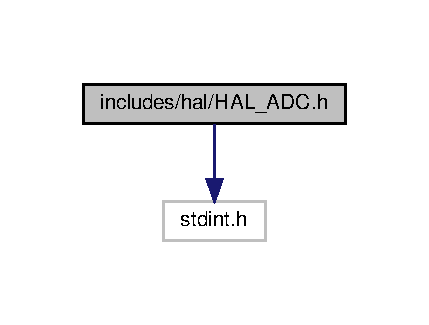
\includegraphics[width=206pt]{HAL__ADC_8h__incl}
\end{center}
\end{figure}
Gráfico de los archivos que directa o indirectamente incluyen a este archivo\+:\nopagebreak
\begin{figure}[H]
\begin{center}
\leavevmode
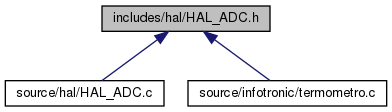
\includegraphics[width=350pt]{HAL__ADC_8h__dep__incl}
\end{center}
\end{figure}
\subsection*{Estructuras de datos}
\begin{DoxyCompactItemize}
\item 
struct \hyperlink{structhal__adc__sequence__config__t}{hal\+\_\+adc\+\_\+sequence\+\_\+config\+\_\+t}
\item 
struct \hyperlink{group__ADC_structhal__adc__sequence__result__t}{hal\+\_\+adc\+\_\+sequence\+\_\+result\+\_\+t}
\end{DoxyCompactItemize}
\subsection*{Enumeraciones}
\begin{DoxyCompactItemize}
\item 
enum \hyperlink{group__ADC_gaee7bd99d368af2a425a9954a9e811a51}{hal\+\_\+adc\+\_\+clock\+\_\+source\+\_\+en} \{ \hyperlink{group__ADC_ggaee7bd99d368af2a425a9954a9e811a51a75a03c616d0b74267642f2b860b19a4c}{H\+A\+L\+\_\+\+A\+D\+C\+\_\+\+C\+L\+O\+C\+K\+\_\+\+S\+O\+U\+R\+C\+E\+\_\+\+F\+RO} = 0, 
\hyperlink{group__ADC_ggaee7bd99d368af2a425a9954a9e811a51ad8be01dc9a2af6e29ab24f823fc40560}{H\+A\+L\+\_\+\+A\+D\+C\+\_\+\+C\+L\+O\+C\+K\+\_\+\+S\+Y\+S\+\_\+\+P\+LL}
 \}
\item 
enum \hyperlink{group__ADC_gaf1570443ca3570a7ae83b90307bbecca}{hal\+\_\+adc\+\_\+low\+\_\+power\+\_\+mode\+\_\+en} \{ \hyperlink{group__ADC_ggaf1570443ca3570a7ae83b90307bbeccaaf92172fb70ce285c23631cb025b3cd52}{H\+A\+L\+\_\+\+A\+D\+C\+\_\+\+L\+O\+W\+\_\+\+P\+O\+W\+E\+R\+\_\+\+M\+O\+D\+E\+\_\+\+D\+I\+S\+A\+B\+L\+ED} = 0, 
\hyperlink{group__ADC_ggaf1570443ca3570a7ae83b90307bbeccaaf3c25521b4c61b46bfe7771db9370769}{H\+A\+L\+\_\+\+A\+D\+C\+\_\+\+L\+O\+W\+\_\+\+P\+O\+W\+E\+R\+\_\+\+M\+O\+D\+E\+\_\+\+E\+N\+A\+B\+L\+ED}
 \}
\item 
enum \hyperlink{group__ADC_ga9297d7b14d7018a94bce94f0103d8559}{hal\+\_\+adc\+\_\+sequence\+\_\+sel\+\_\+en} \{ \hyperlink{group__ADC_gga9297d7b14d7018a94bce94f0103d8559aa8ec9c3fb5a00f2169651f2b1f63df0f}{H\+A\+L\+\_\+\+A\+D\+C\+\_\+\+S\+E\+Q\+U\+E\+N\+C\+E\+\_\+\+S\+E\+L\+\_\+A} = 0, 
\hyperlink{group__ADC_gga9297d7b14d7018a94bce94f0103d8559a109de2c585363efee84dbfb7eee7a1c5}{H\+A\+L\+\_\+\+A\+D\+C\+\_\+\+S\+E\+Q\+U\+E\+N\+C\+E\+\_\+\+S\+E\+L\+\_\+B}
 \}
\item 
enum \hyperlink{group__ADC_ga67fe859b54301579f1b1daef874514ca}{hal\+\_\+adc\+\_\+trigger\+\_\+sel\+\_\+en} \{ \newline
\hyperlink{group__ADC_gga67fe859b54301579f1b1daef874514caaaf722f012bd0aa063b595333f9012a20}{H\+A\+L\+\_\+\+A\+D\+C\+\_\+\+T\+R\+I\+G\+G\+E\+R\+\_\+\+S\+E\+L\+\_\+\+N\+O\+NE} = 0, 
\hyperlink{group__ADC_gga67fe859b54301579f1b1daef874514caa2b6bc8f45ca02b89db9d0b827078a8ac}{H\+A\+L\+\_\+\+A\+D\+C\+\_\+\+T\+R\+I\+G\+G\+E\+R\+\_\+\+S\+E\+L\+\_\+\+P\+I\+N\+I\+N\+T0\+\_\+\+I\+RQ}, 
\hyperlink{group__ADC_gga67fe859b54301579f1b1daef874514caa81102caf42db5f4d5f7b958fe7d9ae6d}{H\+A\+L\+\_\+\+A\+D\+C\+\_\+\+T\+R\+I\+G\+G\+E\+R\+\_\+\+S\+E\+L\+\_\+\+P\+I\+N\+I\+N\+T1\+\_\+\+I\+RQ}, 
\hyperlink{group__ADC_gga67fe859b54301579f1b1daef874514caaca0d6e9551dede7c8a6d596930051e1b}{H\+A\+L\+\_\+\+A\+D\+C\+\_\+\+T\+R\+I\+G\+G\+E\+R\+\_\+\+S\+E\+L\+\_\+\+S\+C\+T0\+\_\+\+O\+U\+T3}, 
\newline
\hyperlink{group__ADC_gga67fe859b54301579f1b1daef874514caabd9e6d4d09caa99ca09a5f44e7797559}{H\+A\+L\+\_\+\+A\+D\+C\+\_\+\+T\+R\+I\+G\+G\+E\+R\+\_\+\+S\+E\+L\+\_\+\+S\+C\+T0\+\_\+\+O\+U\+T4}, 
\hyperlink{group__ADC_gga67fe859b54301579f1b1daef874514caaec235477986c69173f0ad5923a108e5c}{H\+A\+L\+\_\+\+A\+D\+C\+\_\+\+T\+R\+I\+G\+G\+E\+R\+\_\+\+S\+E\+L\+\_\+\+T0\+\_\+\+M\+A\+T3}, 
\hyperlink{group__ADC_gga67fe859b54301579f1b1daef874514caa2ad01d053980af503848525f78d777cf}{H\+A\+L\+\_\+\+A\+D\+C\+\_\+\+T\+R\+I\+G\+G\+E\+R\+\_\+\+S\+E\+L\+\_\+\+C\+M\+P0\+\_\+\+O\+U\+T\+\_\+\+A\+DC}, 
\hyperlink{group__ADC_gga67fe859b54301579f1b1daef874514caa6a9b003480c13c98d8cc1f80bf9c83d1}{H\+A\+L\+\_\+\+A\+D\+C\+\_\+\+T\+R\+I\+G\+G\+E\+R\+\_\+\+S\+E\+L\+\_\+\+G\+P\+I\+O\+\_\+\+I\+N\+T\+\_\+\+B\+M\+AT}, 
\newline
\hyperlink{group__ADC_gga67fe859b54301579f1b1daef874514caa246bfa95b40201277d6c5220c7b57d55}{H\+A\+L\+\_\+\+A\+D\+C\+\_\+\+T\+R\+I\+G\+G\+E\+R\+\_\+\+S\+E\+L\+\_\+\+A\+R\+M\+\_\+\+T\+X\+EV}
 \}
\item 
enum \hyperlink{group__ADC_ga4c5aa9e0991c432640845d2aedb971b2}{hal\+\_\+adc\+\_\+trigger\+\_\+pol\+\_\+sel\+\_\+en} \{ \hyperlink{group__ADC_gga4c5aa9e0991c432640845d2aedb971b2a007c22a34504d8557d98704becf95dc8}{H\+A\+L\+\_\+\+A\+D\+C\+\_\+\+T\+R\+I\+G\+G\+E\+R\+\_\+\+P\+O\+L\+\_\+\+S\+E\+L\+\_\+\+N\+E\+G\+A\+T\+I\+V\+E\+\_\+\+E\+D\+GE} = 0, 
\hyperlink{group__ADC_gga4c5aa9e0991c432640845d2aedb971b2a90868bfab7ec6bdbbca671834798002a}{H\+A\+L\+\_\+\+A\+D\+C\+\_\+\+T\+R\+I\+G\+G\+E\+R\+\_\+\+P\+O\+L\+\_\+\+S\+E\+L\+\_\+\+P\+O\+S\+I\+T\+I\+V\+E\+\_\+\+E\+D\+GE}
 \}
\item 
enum \hyperlink{group__ADC_ga8aa0efd767a9edc5a80b80c4061e0904}{hal\+\_\+adc\+\_\+sync\+\_\+sel\+\_\+en} \{ \hyperlink{group__ADC_gga8aa0efd767a9edc5a80b80c4061e0904a9b81d3ee891639da0e3cec4be09aa668}{H\+A\+L\+\_\+\+A\+D\+C\+\_\+\+S\+Y\+N\+C\+\_\+\+S\+E\+L\+\_\+\+E\+N\+A\+B\+L\+E\+\_\+\+S\+Y\+NC} = 0, 
\hyperlink{group__ADC_gga8aa0efd767a9edc5a80b80c4061e0904a1cbf7646bbe7c32e3e21663fc5952d77}{H\+A\+L\+\_\+\+A\+D\+C\+\_\+\+S\+Y\+N\+C\+\_\+\+S\+E\+L\+\_\+\+B\+Y\+P\+A\+S\+S\+\_\+\+S\+Y\+NC}
 \}
\item 
enum \hyperlink{group__ADC_gaf4981172881d597ede49249ba04fcafe}{hal\+\_\+adc\+\_\+interrupt\+\_\+mode\+\_\+en} \{ \hyperlink{group__ADC_ggaf4981172881d597ede49249ba04fcafea5ffa6da6af1258df4a582e682fab937e}{H\+A\+L\+\_\+\+A\+D\+C\+\_\+\+I\+N\+T\+E\+R\+R\+U\+P\+T\+\_\+\+M\+O\+D\+E\+\_\+\+E\+OC} = 0, 
\hyperlink{group__ADC_ggaf4981172881d597ede49249ba04fcafeae73eff6d5c4ef7297d31a28e4a76e149}{H\+A\+L\+\_\+\+A\+D\+C\+\_\+\+I\+N\+T\+E\+R\+R\+U\+P\+T\+\_\+\+M\+O\+D\+E\+\_\+\+E\+OS}
 \}
\item 
enum \hyperlink{group__ADC_ga99371f47be5b6b4b61c32a1ea86f2b6c}{hal\+\_\+adc\+\_\+result\+\_\+channel\+\_\+en} \{ \newline
\hyperlink{group__ADC_gga99371f47be5b6b4b61c32a1ea86f2b6cae2362f053cdc16412bb073d9b8596c44}{H\+A\+L\+\_\+\+A\+D\+C\+\_\+\+R\+E\+S\+U\+L\+T\+\_\+\+C\+H\+A\+N\+N\+E\+L\+\_\+0} = 0, 
\hyperlink{group__ADC_gga99371f47be5b6b4b61c32a1ea86f2b6cad9342d3898065098fe27e4dcc8a3eb42}{H\+A\+L\+\_\+\+A\+D\+C\+\_\+\+R\+E\+S\+U\+L\+T\+\_\+\+C\+H\+A\+N\+N\+E\+L\+\_\+1}, 
\hyperlink{group__ADC_gga99371f47be5b6b4b61c32a1ea86f2b6ca5d1c958233a386a6c310d9d6a05af99b}{H\+A\+L\+\_\+\+A\+D\+C\+\_\+\+R\+E\+S\+U\+L\+T\+\_\+\+C\+H\+A\+N\+N\+E\+L\+\_\+2}, 
\hyperlink{group__ADC_gga99371f47be5b6b4b61c32a1ea86f2b6ca90074f879325c27fb3e6f3b6457b8cdd}{H\+A\+L\+\_\+\+A\+D\+C\+\_\+\+R\+E\+S\+U\+L\+T\+\_\+\+C\+H\+A\+N\+N\+E\+L\+\_\+3}, 
\newline
\hyperlink{group__ADC_gga99371f47be5b6b4b61c32a1ea86f2b6cad9a84cedc1eb8834223dc1ae6f78f670}{H\+A\+L\+\_\+\+A\+D\+C\+\_\+\+R\+E\+S\+U\+L\+T\+\_\+\+C\+H\+A\+N\+N\+E\+L\+\_\+4}, 
\hyperlink{group__ADC_gga99371f47be5b6b4b61c32a1ea86f2b6cae3c16a8fbe0a0fc75e128f07ba591551}{H\+A\+L\+\_\+\+A\+D\+C\+\_\+\+R\+E\+S\+U\+L\+T\+\_\+\+C\+H\+A\+N\+N\+E\+L\+\_\+5}, 
\hyperlink{group__ADC_gga99371f47be5b6b4b61c32a1ea86f2b6ca9c092202a41a90b27021b181b8095d0c}{H\+A\+L\+\_\+\+A\+D\+C\+\_\+\+R\+E\+S\+U\+L\+T\+\_\+\+C\+H\+A\+N\+N\+E\+L\+\_\+6}, 
\hyperlink{group__ADC_gga99371f47be5b6b4b61c32a1ea86f2b6ca3a9b198659ea511f681900d33c3ba9b5}{H\+A\+L\+\_\+\+A\+D\+C\+\_\+\+R\+E\+S\+U\+L\+T\+\_\+\+C\+H\+A\+N\+N\+E\+L\+\_\+7}, 
\newline
\hyperlink{group__ADC_gga99371f47be5b6b4b61c32a1ea86f2b6cabc4c77b0cea275dd40b1855f82ac6bba}{H\+A\+L\+\_\+\+A\+D\+C\+\_\+\+R\+E\+S\+U\+L\+T\+\_\+\+C\+H\+A\+N\+N\+E\+L\+\_\+8}, 
\hyperlink{group__ADC_gga99371f47be5b6b4b61c32a1ea86f2b6cad33cd49685f140838b575ce39fa26b47}{H\+A\+L\+\_\+\+A\+D\+C\+\_\+\+R\+E\+S\+U\+L\+T\+\_\+\+C\+H\+A\+N\+N\+E\+L\+\_\+9}, 
\hyperlink{group__ADC_gga99371f47be5b6b4b61c32a1ea86f2b6cab81b8df7af28471ac9a6487e88dc0aa8}{H\+A\+L\+\_\+\+A\+D\+C\+\_\+\+R\+E\+S\+U\+L\+T\+\_\+\+C\+H\+A\+N\+N\+E\+L\+\_\+10}, 
\hyperlink{group__ADC_gga99371f47be5b6b4b61c32a1ea86f2b6ca40f8bddc9303b2bae49bb0fcf4dcdf83}{H\+A\+L\+\_\+\+A\+D\+C\+\_\+\+R\+E\+S\+U\+L\+T\+\_\+\+C\+H\+A\+N\+N\+E\+L\+\_\+11}, 
\newline
\hyperlink{group__ADC_gga99371f47be5b6b4b61c32a1ea86f2b6ca5745789eb64375e74e6046b035e92b67}{H\+A\+L\+\_\+\+A\+D\+C\+\_\+\+R\+E\+S\+U\+L\+T\+\_\+\+C\+H\+A\+N\+N\+E\+L\+\_\+\+G\+L\+O\+B\+AL}
 \}
\item 
enum \hyperlink{group__ADC_ga7761986f9c56b809bce1299c6c32eddd}{hal\+\_\+adc\+\_\+sequence\+\_\+result\+\_\+en} \{ \hyperlink{group__ADC_gga7761986f9c56b809bce1299c6c32eddda0c93ff0a1c4ed09ad4b9e1443c4f329f}{H\+A\+L\+\_\+\+A\+D\+C\+\_\+\+S\+E\+Q\+U\+E\+N\+C\+E\+\_\+\+R\+E\+S\+U\+L\+T\+\_\+\+V\+A\+L\+ID} = 0, 
\hyperlink{group__ADC_gga7761986f9c56b809bce1299c6c32edddaec35d0357a3d36bc2c2789d2d45a994e}{H\+A\+L\+\_\+\+A\+D\+C\+\_\+\+S\+E\+Q\+U\+E\+N\+C\+E\+\_\+\+R\+E\+S\+U\+L\+T\+\_\+\+I\+N\+V\+A\+L\+ID}
 \}
\end{DoxyCompactItemize}
\subsection*{Funciones}
\begin{DoxyCompactItemize}
\item 
void \hyperlink{group__ADC_ga4a31179837133973ad68fa993a4e3cd0}{hal\+\_\+adc\+\_\+init\+\_\+async\+\_\+mode} (uint32\+\_\+t sample\+\_\+freq, uint8\+\_\+t div, \hyperlink{group__ADC_gaee7bd99d368af2a425a9954a9e811a51}{hal\+\_\+adc\+\_\+clock\+\_\+source\+\_\+en} clock\+\_\+source, \hyperlink{group__ADC_gaf1570443ca3570a7ae83b90307bbecca}{hal\+\_\+adc\+\_\+low\+\_\+power\+\_\+mode\+\_\+en} low\+\_\+power)
\begin{DoxyCompactList}\small\item\em Inicializar el {\itshape A\+DC} en modo {\bfseries asincrónico}. \end{DoxyCompactList}\item 
void \hyperlink{group__ADC_ga952626700075b275e7766c0095e4ec36}{hal\+\_\+adc\+\_\+init\+\_\+sync\+\_\+mode} (uint32\+\_\+t sample\+\_\+freq, \hyperlink{group__ADC_gaf1570443ca3570a7ae83b90307bbecca}{hal\+\_\+adc\+\_\+low\+\_\+power\+\_\+mode\+\_\+en} low\+\_\+power)
\begin{DoxyCompactList}\small\item\em Inicializar el {\itshape A\+DC} en modo {\bfseries sincrónico}. \end{DoxyCompactList}\item 
void \hyperlink{group__ADC_gab7f00d9f916d45943647ae254ac92d24}{hal\+\_\+adc\+\_\+deinit} (void)
\begin{DoxyCompactList}\small\item\em De-\/inicialización del {\itshape A\+DC}. \end{DoxyCompactList}\item 
void \hyperlink{group__ADC_gadcef726eaa85af74ade96c14f9a48feb}{hal\+\_\+adc\+\_\+config\+\_\+sequence} (\hyperlink{group__ADC_ga9297d7b14d7018a94bce94f0103d8559}{hal\+\_\+adc\+\_\+sequence\+\_\+sel\+\_\+en} sequence, const \hyperlink{structhal__adc__sequence__config__t}{hal\+\_\+adc\+\_\+sequence\+\_\+config\+\_\+t} $\ast$config)
\begin{DoxyCompactList}\small\item\em Configurar una secuencia de conversión. \end{DoxyCompactList}\item 
void \hyperlink{group__ADC_ga678f2df33d79c246b175d0dd36405430}{hal\+\_\+adc\+\_\+enable\+\_\+sequence} (\hyperlink{group__ADC_ga9297d7b14d7018a94bce94f0103d8559}{hal\+\_\+adc\+\_\+sequence\+\_\+sel\+\_\+en} sequence)
\begin{DoxyCompactList}\small\item\em Habilitar una secuencia. \end{DoxyCompactList}\item 
void \hyperlink{group__ADC_ga154950a81b5f589fde0139178ab1dcf3}{hal\+\_\+adc\+\_\+start\+\_\+sequence} (\hyperlink{group__ADC_ga9297d7b14d7018a94bce94f0103d8559}{hal\+\_\+adc\+\_\+sequence\+\_\+sel\+\_\+en} sequence)
\begin{DoxyCompactList}\small\item\em Disparar conversiones en una secuencia. \end{DoxyCompactList}\item 
\hyperlink{group__ADC_ga7761986f9c56b809bce1299c6c32eddd}{hal\+\_\+adc\+\_\+sequence\+\_\+result\+\_\+en} \hyperlink{group__ADC_ga2abe86b92546f8f4726dd65a7a9ddc0d}{hal\+\_\+adc\+\_\+get\+\_\+sequence\+\_\+result} (\hyperlink{group__ADC_ga9297d7b14d7018a94bce94f0103d8559}{hal\+\_\+adc\+\_\+sequence\+\_\+sel\+\_\+en} sequence, \hyperlink{group__ADC_structhal__adc__sequence__result__t}{hal\+\_\+adc\+\_\+sequence\+\_\+result\+\_\+t} $\ast$result\mbox{[}$\,$\mbox{]})
\begin{DoxyCompactList}\small\item\em Obtener resultado de la secuencia. \end{DoxyCompactList}\end{DoxyCompactItemize}


\subsection{Descripción detallada}
Declaraciones a nivel de aplicacion del periferico A\+DC (L\+P\+C845) 

\begin{DoxyAuthor}{Autor}
Augusto Santini 
\end{DoxyAuthor}
\begin{DoxyDate}{Fecha}
3/2020 
\end{DoxyDate}
\begin{DoxyVersion}{Versión}
1.\+0 
\end{DoxyVersion}

\hypertarget{HAL__CTIMER_8h}{}\section{Referencia del Archivo includes/hal/\+H\+A\+L\+\_\+\+C\+T\+I\+M\+ER.h}
\label{HAL__CTIMER_8h}\index{includes/hal/\+H\+A\+L\+\_\+\+C\+T\+I\+M\+E\+R.\+h@{includes/hal/\+H\+A\+L\+\_\+\+C\+T\+I\+M\+E\+R.\+h}}


Declaraciones a nivel de aplicacion del periferico C\+T\+I\+M\+ER (L\+P\+C845)  


{\ttfamily \#include $<$stdint.\+h$>$}\newline
{\ttfamily \#include $<$H\+A\+L\+\_\+\+G\+P\+I\+O.\+h$>$}\newline
Dependencia gráfica adjunta para H\+A\+L\+\_\+\+C\+T\+I\+M\+E\+R.\+h\+:
\nopagebreak
\begin{figure}[H]
\begin{center}
\leavevmode
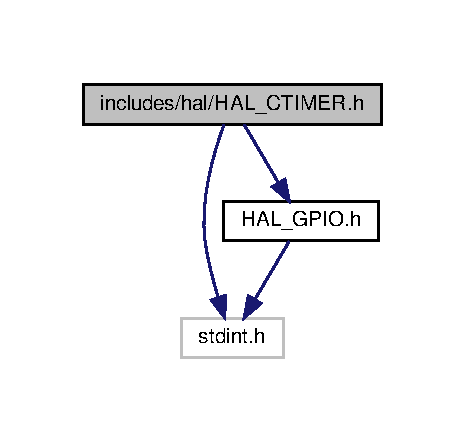
\includegraphics[width=223pt]{HAL__CTIMER_8h__incl}
\end{center}
\end{figure}
\subsection*{Estructuras de datos}
\begin{DoxyCompactItemize}
\item 
struct \hyperlink{structhal__ctimer__match__config__t}{hal\+\_\+ctimer\+\_\+match\+\_\+config\+\_\+t}
\item 
struct \hyperlink{structhal__ctimer__pwm__channel__config__t}{hal\+\_\+ctimer\+\_\+pwm\+\_\+channel\+\_\+config\+\_\+t}
\item 
struct \hyperlink{structhal__ctimer__pwm__config__t}{hal\+\_\+ctimer\+\_\+pwm\+\_\+config\+\_\+t}
\end{DoxyCompactItemize}
\subsection*{Enumeraciones}
\begin{DoxyCompactItemize}
\item 
\mbox{\Hypertarget{HAL__CTIMER_8h_a6aaedba4bb4587f2eacf9e37d4d164bf}\label{HAL__CTIMER_8h_a6aaedba4bb4587f2eacf9e37d4d164bf}} 
enum {\bfseries hal\+\_\+ctimer\+\_\+match\+\_\+action\+\_\+en} \{ {\bfseries H\+A\+L\+\_\+\+C\+T\+I\+M\+E\+R\+\_\+\+M\+A\+T\+C\+H\+\_\+\+D\+O\+\_\+\+N\+O\+G\+H\+I\+NG} = 0, 
{\bfseries H\+A\+L\+\_\+\+C\+T\+I\+M\+E\+R\+\_\+\+M\+A\+T\+C\+H\+\_\+\+C\+L\+E\+A\+R\+\_\+\+P\+IN}, 
{\bfseries H\+A\+L\+\_\+\+C\+T\+I\+M\+E\+R\+\_\+\+M\+A\+T\+C\+H\+\_\+\+S\+E\+T\+\_\+\+P\+IN}, 
{\bfseries H\+A\+L\+\_\+\+C\+T\+I\+M\+E\+R\+\_\+\+M\+A\+T\+C\+H\+\_\+\+T\+O\+G\+G\+L\+E\+\_\+\+P\+IN}
 \}
\item 
\mbox{\Hypertarget{HAL__CTIMER_8h_aeb49458e605ad9b4591fc0a367df2f3f}\label{HAL__CTIMER_8h_aeb49458e605ad9b4591fc0a367df2f3f}} 
enum {\bfseries hal\+\_\+ctimer\+\_\+match\+\_\+sel\+\_\+en} \{ {\bfseries H\+A\+L\+\_\+\+C\+T\+I\+M\+E\+R\+\_\+\+M\+A\+T\+C\+H\+\_\+0} = 0, 
{\bfseries H\+A\+L\+\_\+\+C\+T\+I\+M\+E\+R\+\_\+\+M\+A\+T\+C\+H\+\_\+1}, 
{\bfseries H\+A\+L\+\_\+\+C\+T\+I\+M\+E\+R\+\_\+\+M\+A\+T\+C\+H\+\_\+2}, 
{\bfseries H\+A\+L\+\_\+\+C\+T\+I\+M\+E\+R\+\_\+\+M\+A\+T\+C\+H\+\_\+3}
 \}
\item 
\mbox{\Hypertarget{HAL__CTIMER_8h_a96a7ca81e59a07810e0f9450b9daa8c1}\label{HAL__CTIMER_8h_a96a7ca81e59a07810e0f9450b9daa8c1}} 
enum {\bfseries hal\+\_\+ctimer\+\_\+pwm\+\_\+channel\+\_\+sel\+\_\+en} \{ {\bfseries H\+A\+L\+\_\+\+C\+T\+I\+M\+E\+R\+\_\+\+P\+W\+M\+\_\+\+C\+H\+A\+N\+N\+E\+L\+\_\+0} = 0, 
{\bfseries H\+A\+L\+\_\+\+C\+T\+I\+M\+E\+R\+\_\+\+P\+W\+M\+\_\+\+C\+H\+A\+N\+N\+E\+L\+\_\+1}, 
{\bfseries H\+A\+L\+\_\+\+C\+T\+I\+M\+E\+R\+\_\+\+P\+W\+M\+\_\+\+C\+H\+A\+N\+N\+E\+L\+\_\+2}
 \}
\end{DoxyCompactItemize}
\subsection*{Funciones}
\begin{DoxyCompactItemize}
\item 
void \hyperlink{HAL__CTIMER_8h_a4689eed2a9e77b21de79cc9c9769e269}{hal\+\_\+ctimer\+\_\+timer\+\_\+mode\+\_\+init} (uint32\+\_\+t clock\+\_\+div)
\begin{DoxyCompactList}\small\item\em Inicializacion del periferico en modo timer. \end{DoxyCompactList}\item 
void \hyperlink{HAL__CTIMER_8h_a2a68e905c8f05c550bf06e34f4a1484e}{hal\+\_\+ctimer\+\_\+timer\+\_\+mode\+\_\+config\+\_\+match} (hal\+\_\+ctimer\+\_\+match\+\_\+sel\+\_\+en match\+\_\+sel, const \hyperlink{structhal__ctimer__match__config__t}{hal\+\_\+ctimer\+\_\+match\+\_\+config\+\_\+t} $\ast$match\+\_\+config)
\begin{DoxyCompactList}\small\item\em Configurar un canal de match. \end{DoxyCompactList}\item 
\mbox{\Hypertarget{HAL__CTIMER_8h_a803fbca6afb0855021986d204ffa4b9f}\label{HAL__CTIMER_8h_a803fbca6afb0855021986d204ffa4b9f}} 
void \hyperlink{HAL__CTIMER_8h_a803fbca6afb0855021986d204ffa4b9f}{hal\+\_\+ctimer\+\_\+timer\+\_\+mode\+\_\+run} (void)
\begin{DoxyCompactList}\small\item\em Habilitar el conteo del ctimer. \end{DoxyCompactList}\item 
\mbox{\Hypertarget{HAL__CTIMER_8h_ad855b264d39d920aee8be3c9a0a37db6}\label{HAL__CTIMER_8h_ad855b264d39d920aee8be3c9a0a37db6}} 
void \hyperlink{HAL__CTIMER_8h_ad855b264d39d920aee8be3c9a0a37db6}{hal\+\_\+ctimer\+\_\+timer\+\_\+mode\+\_\+stop} (void)
\begin{DoxyCompactList}\small\item\em Inhabilitar el conteo del ctimer. \end{DoxyCompactList}\item 
\mbox{\Hypertarget{HAL__CTIMER_8h_adc1257569aeffe26a73a3f1af6417d12}\label{HAL__CTIMER_8h_adc1257569aeffe26a73a3f1af6417d12}} 
void \hyperlink{HAL__CTIMER_8h_adc1257569aeffe26a73a3f1af6417d12}{hal\+\_\+ctimer\+\_\+timer\+\_\+mode\+\_\+reset} (void)
\begin{DoxyCompactList}\small\item\em Reiniciar el conteo del ctimer. \end{DoxyCompactList}\item 
void \hyperlink{HAL__CTIMER_8h_a1629367b79d8b3e0fb2769e0b2b96e9c}{hal\+\_\+ctimer\+\_\+pwm\+\_\+mode\+\_\+init} (const \hyperlink{structhal__ctimer__pwm__config__t}{hal\+\_\+ctimer\+\_\+pwm\+\_\+config\+\_\+t} $\ast$config)
\begin{DoxyCompactList}\small\item\em Inicializar el C\+T\+I\+M\+ER en modo P\+WM. \end{DoxyCompactList}\item 
void \hyperlink{HAL__CTIMER_8h_a722302303f22f47995cc6d48bfa1533f}{hal\+\_\+ctimer\+\_\+pwm\+\_\+mode\+\_\+set\+\_\+period} (uint32\+\_\+t period\+\_\+useg)
\begin{DoxyCompactList}\small\item\em Actualizar el periodo en modo P\+WM. \end{DoxyCompactList}\item 
void \hyperlink{HAL__CTIMER_8h_a767f590f1745869d37f7d94a7873280b}{hal\+\_\+ctimer\+\_\+pwm\+\_\+mode\+\_\+config\+\_\+channel} (hal\+\_\+ctimer\+\_\+pwm\+\_\+channel\+\_\+sel\+\_\+en channel\+\_\+sel, const \hyperlink{structhal__ctimer__pwm__channel__config__t}{hal\+\_\+ctimer\+\_\+pwm\+\_\+channel\+\_\+config\+\_\+t} $\ast$channel\+\_\+config)
\begin{DoxyCompactList}\small\item\em Actualizar configuracion de algun canal de P\+WM. \end{DoxyCompactList}\end{DoxyCompactItemize}


\subsection{Descripción detallada}
Declaraciones a nivel de aplicacion del periferico C\+T\+I\+M\+ER (L\+P\+C845) 

\begin{DoxyAuthor}{Autor}
Augusto Santini 
\end{DoxyAuthor}
\begin{DoxyDate}{Fecha}
3/2020 
\end{DoxyDate}
\begin{DoxyVersion}{Versión}
1.\+0 
\end{DoxyVersion}


\subsection{Documentación de las funciones}
\mbox{\Hypertarget{HAL__CTIMER_8h_a4689eed2a9e77b21de79cc9c9769e269}\label{HAL__CTIMER_8h_a4689eed2a9e77b21de79cc9c9769e269}} 
\index{H\+A\+L\+\_\+\+C\+T\+I\+M\+E\+R.\+h@{H\+A\+L\+\_\+\+C\+T\+I\+M\+E\+R.\+h}!hal\+\_\+ctimer\+\_\+timer\+\_\+mode\+\_\+init@{hal\+\_\+ctimer\+\_\+timer\+\_\+mode\+\_\+init}}
\index{hal\+\_\+ctimer\+\_\+timer\+\_\+mode\+\_\+init@{hal\+\_\+ctimer\+\_\+timer\+\_\+mode\+\_\+init}!H\+A\+L\+\_\+\+C\+T\+I\+M\+E\+R.\+h@{H\+A\+L\+\_\+\+C\+T\+I\+M\+E\+R.\+h}}
\subsubsection{\texorpdfstring{hal\+\_\+ctimer\+\_\+timer\+\_\+mode\+\_\+init()}{hal\_ctimer\_timer\_mode\_init()}}
{\footnotesize\ttfamily void hal\+\_\+ctimer\+\_\+timer\+\_\+mode\+\_\+init (\begin{DoxyParamCaption}\item[{uint32\+\_\+t}]{clock\+\_\+div }\end{DoxyParamCaption})}



Inicializacion del periferico en modo timer. 

Esta funcion no pone a correr el contador.


\begin{DoxyParams}[1]{Parámetros}
\mbox{\tt in}  & {\em clock\+\_\+div} & Divisor del clock principal deseado (el valor efectivo es este valor + 1) \\
\hline
\end{DoxyParams}
\mbox{\Hypertarget{HAL__CTIMER_8h_a2a68e905c8f05c550bf06e34f4a1484e}\label{HAL__CTIMER_8h_a2a68e905c8f05c550bf06e34f4a1484e}} 
\index{H\+A\+L\+\_\+\+C\+T\+I\+M\+E\+R.\+h@{H\+A\+L\+\_\+\+C\+T\+I\+M\+E\+R.\+h}!hal\+\_\+ctimer\+\_\+timer\+\_\+mode\+\_\+config\+\_\+match@{hal\+\_\+ctimer\+\_\+timer\+\_\+mode\+\_\+config\+\_\+match}}
\index{hal\+\_\+ctimer\+\_\+timer\+\_\+mode\+\_\+config\+\_\+match@{hal\+\_\+ctimer\+\_\+timer\+\_\+mode\+\_\+config\+\_\+match}!H\+A\+L\+\_\+\+C\+T\+I\+M\+E\+R.\+h@{H\+A\+L\+\_\+\+C\+T\+I\+M\+E\+R.\+h}}
\subsubsection{\texorpdfstring{hal\+\_\+ctimer\+\_\+timer\+\_\+mode\+\_\+config\+\_\+match()}{hal\_ctimer\_timer\_mode\_config\_match()}}
{\footnotesize\ttfamily void hal\+\_\+ctimer\+\_\+timer\+\_\+mode\+\_\+config\+\_\+match (\begin{DoxyParamCaption}\item[{hal\+\_\+ctimer\+\_\+match\+\_\+sel\+\_\+en}]{match\+\_\+sel,  }\item[{const \hyperlink{structhal__ctimer__match__config__t}{hal\+\_\+ctimer\+\_\+match\+\_\+config\+\_\+t} $\ast$}]{match\+\_\+config }\end{DoxyParamCaption})}



Configurar un canal de match. 


\begin{DoxyParams}[1]{Parámetros}
\mbox{\tt in}  & {\em match\+\_\+sel} & Match a configurar \\
\hline
\mbox{\tt in}  & {\em match\+\_\+config} & Configuracion deseada \\
\hline
\end{DoxyParams}
\mbox{\Hypertarget{HAL__CTIMER_8h_a1629367b79d8b3e0fb2769e0b2b96e9c}\label{HAL__CTIMER_8h_a1629367b79d8b3e0fb2769e0b2b96e9c}} 
\index{H\+A\+L\+\_\+\+C\+T\+I\+M\+E\+R.\+h@{H\+A\+L\+\_\+\+C\+T\+I\+M\+E\+R.\+h}!hal\+\_\+ctimer\+\_\+pwm\+\_\+mode\+\_\+init@{hal\+\_\+ctimer\+\_\+pwm\+\_\+mode\+\_\+init}}
\index{hal\+\_\+ctimer\+\_\+pwm\+\_\+mode\+\_\+init@{hal\+\_\+ctimer\+\_\+pwm\+\_\+mode\+\_\+init}!H\+A\+L\+\_\+\+C\+T\+I\+M\+E\+R.\+h@{H\+A\+L\+\_\+\+C\+T\+I\+M\+E\+R.\+h}}
\subsubsection{\texorpdfstring{hal\+\_\+ctimer\+\_\+pwm\+\_\+mode\+\_\+init()}{hal\_ctimer\_pwm\_mode\_init()}}
{\footnotesize\ttfamily void hal\+\_\+ctimer\+\_\+pwm\+\_\+mode\+\_\+init (\begin{DoxyParamCaption}\item[{const \hyperlink{structhal__ctimer__pwm__config__t}{hal\+\_\+ctimer\+\_\+pwm\+\_\+config\+\_\+t} $\ast$}]{config }\end{DoxyParamCaption})}



Inicializar el C\+T\+I\+M\+ER en modo P\+WM. 


\begin{DoxyParams}[1]{Parámetros}
\mbox{\tt in}  & {\em config} & Configuracion deseada \\
\hline
\end{DoxyParams}
\mbox{\Hypertarget{HAL__CTIMER_8h_a722302303f22f47995cc6d48bfa1533f}\label{HAL__CTIMER_8h_a722302303f22f47995cc6d48bfa1533f}} 
\index{H\+A\+L\+\_\+\+C\+T\+I\+M\+E\+R.\+h@{H\+A\+L\+\_\+\+C\+T\+I\+M\+E\+R.\+h}!hal\+\_\+ctimer\+\_\+pwm\+\_\+mode\+\_\+set\+\_\+period@{hal\+\_\+ctimer\+\_\+pwm\+\_\+mode\+\_\+set\+\_\+period}}
\index{hal\+\_\+ctimer\+\_\+pwm\+\_\+mode\+\_\+set\+\_\+period@{hal\+\_\+ctimer\+\_\+pwm\+\_\+mode\+\_\+set\+\_\+period}!H\+A\+L\+\_\+\+C\+T\+I\+M\+E\+R.\+h@{H\+A\+L\+\_\+\+C\+T\+I\+M\+E\+R.\+h}}
\subsubsection{\texorpdfstring{hal\+\_\+ctimer\+\_\+pwm\+\_\+mode\+\_\+set\+\_\+period()}{hal\_ctimer\_pwm\_mode\_set\_period()}}
{\footnotesize\ttfamily void hal\+\_\+ctimer\+\_\+pwm\+\_\+mode\+\_\+set\+\_\+period (\begin{DoxyParamCaption}\item[{uint32\+\_\+t}]{period\+\_\+useg }\end{DoxyParamCaption})}



Actualizar el periodo en modo P\+WM. 


\begin{DoxyParams}[1]{Parámetros}
\mbox{\tt in}  & {\em period\+\_\+useg} & Nuevo periodo deseado en microsegundos \\
\hline
\end{DoxyParams}
\mbox{\Hypertarget{HAL__CTIMER_8h_a767f590f1745869d37f7d94a7873280b}\label{HAL__CTIMER_8h_a767f590f1745869d37f7d94a7873280b}} 
\index{H\+A\+L\+\_\+\+C\+T\+I\+M\+E\+R.\+h@{H\+A\+L\+\_\+\+C\+T\+I\+M\+E\+R.\+h}!hal\+\_\+ctimer\+\_\+pwm\+\_\+mode\+\_\+config\+\_\+channel@{hal\+\_\+ctimer\+\_\+pwm\+\_\+mode\+\_\+config\+\_\+channel}}
\index{hal\+\_\+ctimer\+\_\+pwm\+\_\+mode\+\_\+config\+\_\+channel@{hal\+\_\+ctimer\+\_\+pwm\+\_\+mode\+\_\+config\+\_\+channel}!H\+A\+L\+\_\+\+C\+T\+I\+M\+E\+R.\+h@{H\+A\+L\+\_\+\+C\+T\+I\+M\+E\+R.\+h}}
\subsubsection{\texorpdfstring{hal\+\_\+ctimer\+\_\+pwm\+\_\+mode\+\_\+config\+\_\+channel()}{hal\_ctimer\_pwm\_mode\_config\_channel()}}
{\footnotesize\ttfamily void hal\+\_\+ctimer\+\_\+pwm\+\_\+mode\+\_\+config\+\_\+channel (\begin{DoxyParamCaption}\item[{hal\+\_\+ctimer\+\_\+pwm\+\_\+channel\+\_\+sel\+\_\+en}]{channel\+\_\+sel,  }\item[{const \hyperlink{structhal__ctimer__pwm__channel__config__t}{hal\+\_\+ctimer\+\_\+pwm\+\_\+channel\+\_\+config\+\_\+t} $\ast$}]{channel\+\_\+config }\end{DoxyParamCaption})}



Actualizar configuracion de algun canal de P\+WM. 


\begin{DoxyParams}[1]{Parámetros}
\mbox{\tt in}  & {\em channel\+\_\+sel} & Seleccion de canal a configurar \\
\hline
\mbox{\tt in}  & {\em channel\+\_\+config} & Configuracion del canal de P\+WM \\
\hline
\end{DoxyParams}

\hypertarget{HAL__DAC_8h}{}\section{Referencia del Archivo includes/hal/\+H\+A\+L\+\_\+\+D\+AC.h}
\label{HAL__DAC_8h}\index{includes/hal/\+H\+A\+L\+\_\+\+D\+A\+C.\+h@{includes/hal/\+H\+A\+L\+\_\+\+D\+A\+C.\+h}}


Declaraciones a nivel de aplicacion del periferico D\+AC (L\+P\+C845)  


{\ttfamily \#include $<$stdint.\+h$>$}\newline
Dependencia gráfica adjunta para H\+A\+L\+\_\+\+D\+A\+C.\+h\+:
\nopagebreak
\begin{figure}[H]
\begin{center}
\leavevmode
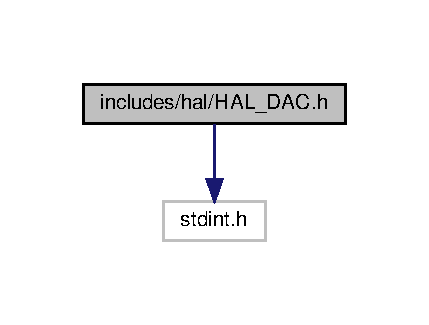
\includegraphics[width=206pt]{HAL__DAC_8h__incl}
\end{center}
\end{figure}
\subsection*{Estructuras de datos}
\begin{DoxyCompactItemize}
\item 
struct \hyperlink{HAL__DAC_8h_structhal__dac__ctrl__config__t}{hal\+\_\+dac\+\_\+ctrl\+\_\+config\+\_\+t}
\end{DoxyCompactItemize}
\subsection*{Enumeraciones}
\begin{DoxyCompactItemize}
\item 
\mbox{\Hypertarget{HAL__DAC_8h_a36a28cc0fff9972f139b7b4959f691e9}\label{HAL__DAC_8h_a36a28cc0fff9972f139b7b4959f691e9}} 
enum {\bfseries hal\+\_\+dac\+\_\+en} \{ {\bfseries H\+A\+L\+\_\+\+D\+A\+C\+\_\+0} = 0, 
{\bfseries H\+A\+L\+\_\+\+D\+A\+C\+\_\+1}
 \}
\item 
\mbox{\Hypertarget{HAL__DAC_8h_a060451e91c937afba2be341b4a8a78c6}\label{HAL__DAC_8h_a060451e91c937afba2be341b4a8a78c6}} 
enum {\bfseries hal\+\_\+dac\+\_\+settling\+\_\+time\+\_\+en} \{ {\bfseries H\+A\+L\+\_\+\+D\+A\+C\+\_\+\+S\+E\+T\+T\+L\+I\+N\+G\+\_\+\+T\+I\+M\+E\+\_\+1\+U\+S\+\_\+\+M\+AX} = 0, 
{\bfseries H\+A\+L\+\_\+\+D\+A\+C\+\_\+\+S\+E\+T\+T\+L\+I\+N\+G\+\_\+\+T\+I\+M\+E\+\_\+2\+\_\+5\+U\+S\+\_\+\+M\+AX}
 \}
\end{DoxyCompactItemize}
\subsection*{Funciones}
\begin{DoxyCompactItemize}
\item 
void \hyperlink{HAL__DAC_8h_a0c3bc10289bf53d637dcf325983d64b9}{hal\+\_\+dac\+\_\+init} (hal\+\_\+dac\+\_\+en dac, hal\+\_\+dac\+\_\+settling\+\_\+time\+\_\+en settling\+\_\+time, uint32\+\_\+t initial\+\_\+value)
\begin{DoxyCompactList}\small\item\em Inicializacion del D\+AC. \end{DoxyCompactList}\end{DoxyCompactItemize}


\subsection{Descripción detallada}
Declaraciones a nivel de aplicacion del periferico D\+AC (L\+P\+C845) 

\begin{DoxyAuthor}{Autor}
Augusto Santini 
\end{DoxyAuthor}
\begin{DoxyDate}{Fecha}
3/2020 
\end{DoxyDate}
\begin{DoxyVersion}{Versión}
1.\+0 
\end{DoxyVersion}


\subsection{Documentación de las estructuras de datos}
\index{hal\+\_\+dac\+\_\+ctrl\+\_\+config\+\_\+t@{hal\+\_\+dac\+\_\+ctrl\+\_\+config\+\_\+t}}\label{structhal__dac__ctrl__config__t}
\Hypertarget{HAL__DAC_8h_structhal__dac__ctrl__config__t}
\subsubsection{struct hal\+\_\+dac\+\_\+ctrl\+\_\+config\+\_\+t}
\begin{DoxyFields}{Campos de datos}
\mbox{\Hypertarget{HAL__DAC_8h_a3dfe52d3dda993a8648198e3957bbdcb}\label{HAL__DAC_8h_a3dfe52d3dda993a8648198e3957bbdcb}} 
uint8\_t&
count\_enable: 1&
\\
\hline

\mbox{\Hypertarget{HAL__DAC_8h_ace4cbb1d9df61bad809887daafeb3262}\label{HAL__DAC_8h_ace4cbb1d9df61bad809887daafeb3262}} 
uint8\_t&
double\_buffering: 1&
\\
\hline

\mbox{\Hypertarget{HAL__DAC_8h_a202a9cec987f30eea0427a8c08966d1f}\label{HAL__DAC_8h_a202a9cec987f30eea0427a8c08966d1f}} 
uint8\_t&
dma\_enable: 1&
\\
\hline

\mbox{\Hypertarget{HAL__DAC_8h_a674aba4c7104bedc212128ae5851d97f}\label{HAL__DAC_8h_a674aba4c7104bedc212128ae5851d97f}} 
uint8\_t&
dma\_request: 1&
\\
\hline

\end{DoxyFields}


\subsection{Documentación de las funciones}
\mbox{\Hypertarget{HAL__DAC_8h_a0c3bc10289bf53d637dcf325983d64b9}\label{HAL__DAC_8h_a0c3bc10289bf53d637dcf325983d64b9}} 
\index{H\+A\+L\+\_\+\+D\+A\+C.\+h@{H\+A\+L\+\_\+\+D\+A\+C.\+h}!hal\+\_\+dac\+\_\+init@{hal\+\_\+dac\+\_\+init}}
\index{hal\+\_\+dac\+\_\+init@{hal\+\_\+dac\+\_\+init}!H\+A\+L\+\_\+\+D\+A\+C.\+h@{H\+A\+L\+\_\+\+D\+A\+C.\+h}}
\subsubsection{\texorpdfstring{hal\+\_\+dac\+\_\+init()}{hal\_dac\_init()}}
{\footnotesize\ttfamily void hal\+\_\+dac\+\_\+init (\begin{DoxyParamCaption}\item[{hal\+\_\+dac\+\_\+en}]{dac,  }\item[{hal\+\_\+dac\+\_\+settling\+\_\+time\+\_\+en}]{settling\+\_\+time,  }\item[{uint32\+\_\+t}]{initial\+\_\+value }\end{DoxyParamCaption})}



Inicializacion del D\+AC. 


\begin{DoxyParams}[1]{Parámetros}
\mbox{\tt in}  & {\em dac} & Cual de los dos D\+A\+Cs inicializar \\
\hline
\mbox{\tt in}  & {\em settling\+\_\+time} & Velocidad de conversion del D\+AC \\
\hline
\mbox{\tt in}  & {\em initial\+\_\+value} & Valor inicial del D\+AC \\
\hline
\end{DoxyParams}

\hypertarget{HAL__GPIO_8h}{}\section{Referencia del Archivo includes/hal/\+H\+A\+L\+\_\+\+G\+P\+IO.h}
\label{HAL__GPIO_8h}\index{includes/hal/\+H\+A\+L\+\_\+\+G\+P\+I\+O.\+h@{includes/hal/\+H\+A\+L\+\_\+\+G\+P\+I\+O.\+h}}


Declaraciones a nivel de aplicacion del periferico G\+P\+IO (L\+P\+C845)  


{\ttfamily \#include $<$stdint.\+h$>$}\newline
Dependencia gráfica adjunta para H\+A\+L\+\_\+\+G\+P\+I\+O.\+h\+:\nopagebreak
\begin{figure}[H]
\begin{center}
\leavevmode
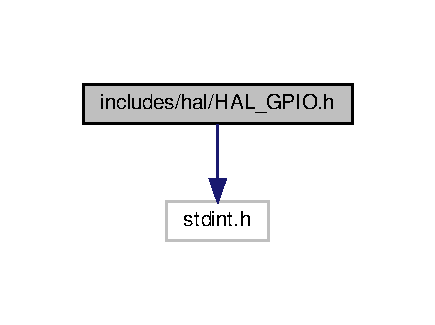
\includegraphics[width=209pt]{HAL__GPIO_8h__incl}
\end{center}
\end{figure}
Gráfico de los archivos que directa o indirectamente incluyen a este archivo\+:\nopagebreak
\begin{figure}[H]
\begin{center}
\leavevmode
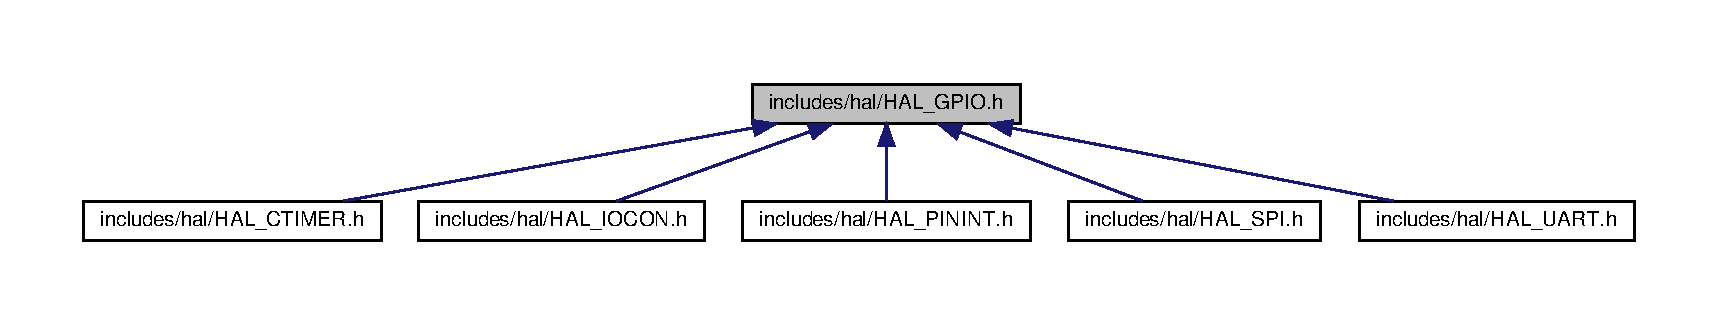
\includegraphics[width=350pt]{HAL__GPIO_8h__dep__incl}
\end{center}
\end{figure}
\subsection*{defines}
\begin{DoxyCompactItemize}
\item 
\mbox{\Hypertarget{HAL__GPIO_8h_ae0a26fe45351d3fab4b1bc5d59a6ea58}\label{HAL__GPIO_8h_ae0a26fe45351d3fab4b1bc5d59a6ea58}} 
\#define {\bfseries H\+A\+L\+\_\+\+G\+P\+I\+O\+\_\+\+P\+O\+R\+T\+P\+I\+N\+\_\+\+T\+O\+\_\+\+P\+O\+RT}(x)~(x / 32)
\item 
\mbox{\Hypertarget{HAL__GPIO_8h_a204f5d369f98d6f5fd068efb03ce09b8}\label{HAL__GPIO_8h_a204f5d369f98d6f5fd068efb03ce09b8}} 
\#define {\bfseries H\+A\+L\+\_\+\+G\+P\+I\+O\+\_\+\+P\+O\+R\+T\+P\+I\+N\+\_\+\+T\+O\+\_\+\+P\+IN}(x)~(x \% 32)
\end{DoxyCompactItemize}
\subsection*{Enumeraciones}
\begin{DoxyCompactItemize}
\item 
\mbox{\Hypertarget{HAL__GPIO_8h_a67db951437d45b48c1504058e8a48302}\label{HAL__GPIO_8h_a67db951437d45b48c1504058e8a48302}} 
enum {\bfseries hal\+\_\+gpio\+\_\+port\+\_\+en} \{ {\bfseries H\+A\+L\+\_\+\+G\+P\+I\+O\+\_\+\+P\+O\+R\+T\+\_\+0} = 0, 
{\bfseries H\+A\+L\+\_\+\+G\+P\+I\+O\+\_\+\+P\+O\+R\+T\+\_\+1}
 \}
\item 
\mbox{\Hypertarget{HAL__GPIO_8h_a5fd48fa8390fc0ec15d4d7f7c2bbc51b}\label{HAL__GPIO_8h_a5fd48fa8390fc0ec15d4d7f7c2bbc51b}} 
enum {\bfseries hal\+\_\+gpio\+\_\+portpin\+\_\+en} \{ \newline
{\bfseries H\+A\+L\+\_\+\+G\+P\+I\+O\+\_\+\+P\+O\+R\+T\+P\+I\+N\+\_\+0\+\_\+0} = 0, 
{\bfseries H\+A\+L\+\_\+\+G\+P\+I\+O\+\_\+\+P\+O\+R\+T\+P\+I\+N\+\_\+0\+\_\+1}, 
{\bfseries H\+A\+L\+\_\+\+G\+P\+I\+O\+\_\+\+P\+O\+R\+T\+P\+I\+N\+\_\+0\+\_\+2}, 
{\bfseries H\+A\+L\+\_\+\+G\+P\+I\+O\+\_\+\+P\+O\+R\+T\+P\+I\+N\+\_\+0\+\_\+3}, 
\newline
{\bfseries H\+A\+L\+\_\+\+G\+P\+I\+O\+\_\+\+P\+O\+R\+T\+P\+I\+N\+\_\+0\+\_\+4}, 
{\bfseries H\+A\+L\+\_\+\+G\+P\+I\+O\+\_\+\+P\+O\+R\+T\+P\+I\+N\+\_\+0\+\_\+5}, 
{\bfseries H\+A\+L\+\_\+\+G\+P\+I\+O\+\_\+\+P\+O\+R\+T\+P\+I\+N\+\_\+0\+\_\+6}, 
{\bfseries H\+A\+L\+\_\+\+G\+P\+I\+O\+\_\+\+P\+O\+R\+T\+P\+I\+N\+\_\+0\+\_\+7}, 
\newline
{\bfseries H\+A\+L\+\_\+\+G\+P\+I\+O\+\_\+\+P\+O\+R\+T\+P\+I\+N\+\_\+0\+\_\+8}, 
{\bfseries H\+A\+L\+\_\+\+G\+P\+I\+O\+\_\+\+P\+O\+R\+T\+P\+I\+N\+\_\+0\+\_\+9}, 
{\bfseries H\+A\+L\+\_\+\+G\+P\+I\+O\+\_\+\+P\+O\+R\+T\+P\+I\+N\+\_\+0\+\_\+10}, 
{\bfseries H\+A\+L\+\_\+\+G\+P\+I\+O\+\_\+\+P\+O\+R\+T\+P\+I\+N\+\_\+0\+\_\+11}, 
\newline
{\bfseries H\+A\+L\+\_\+\+G\+P\+I\+O\+\_\+\+P\+O\+R\+T\+P\+I\+N\+\_\+0\+\_\+12}, 
{\bfseries H\+A\+L\+\_\+\+G\+P\+I\+O\+\_\+\+P\+O\+R\+T\+P\+I\+N\+\_\+0\+\_\+13}, 
{\bfseries H\+A\+L\+\_\+\+G\+P\+I\+O\+\_\+\+P\+O\+R\+T\+P\+I\+N\+\_\+0\+\_\+14}, 
{\bfseries H\+A\+L\+\_\+\+G\+P\+I\+O\+\_\+\+P\+O\+R\+T\+P\+I\+N\+\_\+0\+\_\+15}, 
\newline
{\bfseries H\+A\+L\+\_\+\+G\+P\+I\+O\+\_\+\+P\+O\+R\+T\+P\+I\+N\+\_\+0\+\_\+16}, 
{\bfseries H\+A\+L\+\_\+\+G\+P\+I\+O\+\_\+\+P\+O\+R\+T\+P\+I\+N\+\_\+0\+\_\+17}, 
{\bfseries H\+A\+L\+\_\+\+G\+P\+I\+O\+\_\+\+P\+O\+R\+T\+P\+I\+N\+\_\+0\+\_\+18}, 
{\bfseries H\+A\+L\+\_\+\+G\+P\+I\+O\+\_\+\+P\+O\+R\+T\+P\+I\+N\+\_\+0\+\_\+19}, 
\newline
{\bfseries H\+A\+L\+\_\+\+G\+P\+I\+O\+\_\+\+P\+O\+R\+T\+P\+I\+N\+\_\+0\+\_\+20}, 
{\bfseries H\+A\+L\+\_\+\+G\+P\+I\+O\+\_\+\+P\+O\+R\+T\+P\+I\+N\+\_\+0\+\_\+21}, 
{\bfseries H\+A\+L\+\_\+\+G\+P\+I\+O\+\_\+\+P\+O\+R\+T\+P\+I\+N\+\_\+0\+\_\+22}, 
{\bfseries H\+A\+L\+\_\+\+G\+P\+I\+O\+\_\+\+P\+O\+R\+T\+P\+I\+N\+\_\+0\+\_\+23}, 
\newline
{\bfseries H\+A\+L\+\_\+\+G\+P\+I\+O\+\_\+\+P\+O\+R\+T\+P\+I\+N\+\_\+0\+\_\+24}, 
{\bfseries H\+A\+L\+\_\+\+G\+P\+I\+O\+\_\+\+P\+O\+R\+T\+P\+I\+N\+\_\+0\+\_\+25}, 
{\bfseries H\+A\+L\+\_\+\+G\+P\+I\+O\+\_\+\+P\+O\+R\+T\+P\+I\+N\+\_\+0\+\_\+26}, 
{\bfseries H\+A\+L\+\_\+\+G\+P\+I\+O\+\_\+\+P\+O\+R\+T\+P\+I\+N\+\_\+0\+\_\+27}, 
\newline
{\bfseries H\+A\+L\+\_\+\+G\+P\+I\+O\+\_\+\+P\+O\+R\+T\+P\+I\+N\+\_\+0\+\_\+28}, 
{\bfseries H\+A\+L\+\_\+\+G\+P\+I\+O\+\_\+\+P\+O\+R\+T\+P\+I\+N\+\_\+0\+\_\+29}, 
{\bfseries H\+A\+L\+\_\+\+G\+P\+I\+O\+\_\+\+P\+O\+R\+T\+P\+I\+N\+\_\+0\+\_\+30}, 
{\bfseries H\+A\+L\+\_\+\+G\+P\+I\+O\+\_\+\+P\+O\+R\+T\+P\+I\+N\+\_\+0\+\_\+31}, 
\newline
{\bfseries H\+A\+L\+\_\+\+G\+P\+I\+O\+\_\+\+P\+O\+R\+T\+P\+I\+N\+\_\+1\+\_\+0}, 
{\bfseries H\+A\+L\+\_\+\+G\+P\+I\+O\+\_\+\+P\+O\+R\+T\+P\+I\+N\+\_\+1\+\_\+1}, 
{\bfseries H\+A\+L\+\_\+\+G\+P\+I\+O\+\_\+\+P\+O\+R\+T\+P\+I\+N\+\_\+1\+\_\+2}, 
{\bfseries H\+A\+L\+\_\+\+G\+P\+I\+O\+\_\+\+P\+O\+R\+T\+P\+I\+N\+\_\+1\+\_\+3}, 
\newline
{\bfseries H\+A\+L\+\_\+\+G\+P\+I\+O\+\_\+\+P\+O\+R\+T\+P\+I\+N\+\_\+1\+\_\+4}, 
{\bfseries H\+A\+L\+\_\+\+G\+P\+I\+O\+\_\+\+P\+O\+R\+T\+P\+I\+N\+\_\+1\+\_\+5}, 
{\bfseries H\+A\+L\+\_\+\+G\+P\+I\+O\+\_\+\+P\+O\+R\+T\+P\+I\+N\+\_\+1\+\_\+6}, 
{\bfseries H\+A\+L\+\_\+\+G\+P\+I\+O\+\_\+\+P\+O\+R\+T\+P\+I\+N\+\_\+1\+\_\+7}, 
\newline
{\bfseries H\+A\+L\+\_\+\+G\+P\+I\+O\+\_\+\+P\+O\+R\+T\+P\+I\+N\+\_\+1\+\_\+8}, 
{\bfseries H\+A\+L\+\_\+\+G\+P\+I\+O\+\_\+\+P\+O\+R\+T\+P\+I\+N\+\_\+1\+\_\+9}, 
{\bfseries H\+A\+L\+\_\+\+G\+P\+I\+O\+\_\+\+P\+O\+R\+T\+P\+I\+N\+\_\+\+N\+O\+T\+\_\+\+U\+S\+ED}
 \}
\item 
\mbox{\Hypertarget{HAL__GPIO_8h_acdde9afffdc2043850035540298a5473}\label{HAL__GPIO_8h_acdde9afffdc2043850035540298a5473}} 
enum {\bfseries hal\+\_\+gpio\+\_\+dir\+\_\+en} \{ {\bfseries H\+A\+L\+\_\+\+G\+P\+I\+O\+\_\+\+D\+I\+R\+\_\+\+I\+N\+P\+UT} = 0, 
{\bfseries H\+A\+L\+\_\+\+G\+P\+I\+O\+\_\+\+D\+I\+R\+\_\+\+O\+U\+T\+P\+UT}
 \}
\end{DoxyCompactItemize}
\subsection*{Funciones}
\begin{DoxyCompactItemize}
\item 
void \hyperlink{HAL__GPIO_8h_a315deab93915cc375acef1e81046f2bc}{hal\+\_\+gpio\+\_\+init} (hal\+\_\+gpio\+\_\+port\+\_\+en port)
\begin{DoxyCompactList}\small\item\em Inicializar un puerto. \end{DoxyCompactList}\item 
void \hyperlink{HAL__GPIO_8h_a88843594aedf65f8f0c97eade8853124}{hal\+\_\+gpio\+\_\+set\+\_\+dir} (hal\+\_\+gpio\+\_\+portpin\+\_\+en portpin, hal\+\_\+gpio\+\_\+dir\+\_\+en dir, uint8\+\_\+t initial\+\_\+state)
\begin{DoxyCompactList}\small\item\em Fijar direccion de una G\+P\+IO. \end{DoxyCompactList}\item 
void \hyperlink{HAL__GPIO_8h_abb1f2e1042b1fe64677f95a439076527}{hal\+\_\+gpio\+\_\+set\+\_\+pin} (hal\+\_\+gpio\+\_\+portpin\+\_\+en portpin)
\begin{DoxyCompactList}\small\item\em Fijar estado activo de una G\+P\+IO. \end{DoxyCompactList}\item 
void \hyperlink{HAL__GPIO_8h_acdea7b3a5bae213e58bce78fb5356eb2}{hal\+\_\+gpio\+\_\+clear\+\_\+pin} (hal\+\_\+gpio\+\_\+portpin\+\_\+en portpin)
\begin{DoxyCompactList}\small\item\em Fijar estado inactivo de una G\+P\+IO. \end{DoxyCompactList}\item 
void \hyperlink{HAL__GPIO_8h_a3c6ea73afbcc76405ef5c6ac22bc57ac}{hal\+\_\+gpio\+\_\+toggle\+\_\+pin} (hal\+\_\+gpio\+\_\+portpin\+\_\+en portpin)
\begin{DoxyCompactList}\small\item\em Invertir estado de una G\+P\+IO. \end{DoxyCompactList}\item 
uint8\+\_\+t \hyperlink{HAL__GPIO_8h_a84780bdc959ae4cc21cdc2fd063a1ed6}{hal\+\_\+gpio\+\_\+read\+\_\+pin} (hal\+\_\+gpio\+\_\+portpin\+\_\+en portpin)
\begin{DoxyCompactList}\small\item\em Leer el estado de una G\+P\+IO. \end{DoxyCompactList}\end{DoxyCompactItemize}


\subsection{Descripción detallada}
Declaraciones a nivel de aplicacion del periferico G\+P\+IO (L\+P\+C845) 

\begin{DoxyAuthor}{Autor}
Augusto Santini 
\end{DoxyAuthor}
\begin{DoxyDate}{Fecha}
3/2020 
\end{DoxyDate}
\begin{DoxyVersion}{Versión}
1.\+0 
\end{DoxyVersion}


\subsection{Documentación de las funciones}
\mbox{\Hypertarget{HAL__GPIO_8h_a315deab93915cc375acef1e81046f2bc}\label{HAL__GPIO_8h_a315deab93915cc375acef1e81046f2bc}} 
\index{H\+A\+L\+\_\+\+G\+P\+I\+O.\+h@{H\+A\+L\+\_\+\+G\+P\+I\+O.\+h}!hal\+\_\+gpio\+\_\+init@{hal\+\_\+gpio\+\_\+init}}
\index{hal\+\_\+gpio\+\_\+init@{hal\+\_\+gpio\+\_\+init}!H\+A\+L\+\_\+\+G\+P\+I\+O.\+h@{H\+A\+L\+\_\+\+G\+P\+I\+O.\+h}}
\subsubsection{\texorpdfstring{hal\+\_\+gpio\+\_\+init()}{hal\_gpio\_init()}}
{\footnotesize\ttfamily void hal\+\_\+gpio\+\_\+init (\begin{DoxyParamCaption}\item[{hal\+\_\+gpio\+\_\+port\+\_\+en}]{port }\end{DoxyParamCaption})}



Inicializar un puerto. 


\begin{DoxyParams}[1]{Parámetros}
\mbox{\tt in}  & {\em port} & Puerto a inicializar \\
\hline
\end{DoxyParams}
\mbox{\Hypertarget{HAL__GPIO_8h_a88843594aedf65f8f0c97eade8853124}\label{HAL__GPIO_8h_a88843594aedf65f8f0c97eade8853124}} 
\index{H\+A\+L\+\_\+\+G\+P\+I\+O.\+h@{H\+A\+L\+\_\+\+G\+P\+I\+O.\+h}!hal\+\_\+gpio\+\_\+set\+\_\+dir@{hal\+\_\+gpio\+\_\+set\+\_\+dir}}
\index{hal\+\_\+gpio\+\_\+set\+\_\+dir@{hal\+\_\+gpio\+\_\+set\+\_\+dir}!H\+A\+L\+\_\+\+G\+P\+I\+O.\+h@{H\+A\+L\+\_\+\+G\+P\+I\+O.\+h}}
\subsubsection{\texorpdfstring{hal\+\_\+gpio\+\_\+set\+\_\+dir()}{hal\_gpio\_set\_dir()}}
{\footnotesize\ttfamily void hal\+\_\+gpio\+\_\+set\+\_\+dir (\begin{DoxyParamCaption}\item[{hal\+\_\+gpio\+\_\+portpin\+\_\+en}]{portpin,  }\item[{hal\+\_\+gpio\+\_\+dir\+\_\+en}]{dir,  }\item[{uint8\+\_\+t}]{initial\+\_\+state }\end{DoxyParamCaption})}



Fijar direccion de una G\+P\+IO. 


\begin{DoxyParams}[1]{Parámetros}
\mbox{\tt in}  & {\em portpin} & Numero de puerto/pin a configurar \\
\hline
\mbox{\tt in}  & {\em dir} & Direccion deseada \\
\hline
\mbox{\tt in}  & {\em initial\+\_\+state} & Estado inicial (aplica para salidas nada mas) \\
\hline
\end{DoxyParams}
\mbox{\Hypertarget{HAL__GPIO_8h_abb1f2e1042b1fe64677f95a439076527}\label{HAL__GPIO_8h_abb1f2e1042b1fe64677f95a439076527}} 
\index{H\+A\+L\+\_\+\+G\+P\+I\+O.\+h@{H\+A\+L\+\_\+\+G\+P\+I\+O.\+h}!hal\+\_\+gpio\+\_\+set\+\_\+pin@{hal\+\_\+gpio\+\_\+set\+\_\+pin}}
\index{hal\+\_\+gpio\+\_\+set\+\_\+pin@{hal\+\_\+gpio\+\_\+set\+\_\+pin}!H\+A\+L\+\_\+\+G\+P\+I\+O.\+h@{H\+A\+L\+\_\+\+G\+P\+I\+O.\+h}}
\subsubsection{\texorpdfstring{hal\+\_\+gpio\+\_\+set\+\_\+pin()}{hal\_gpio\_set\_pin()}}
{\footnotesize\ttfamily void hal\+\_\+gpio\+\_\+set\+\_\+pin (\begin{DoxyParamCaption}\item[{hal\+\_\+gpio\+\_\+portpin\+\_\+en}]{portpin }\end{DoxyParamCaption})}



Fijar estado activo de una G\+P\+IO. 


\begin{DoxyParams}[1]{Parámetros}
\mbox{\tt in}  & {\em portpin} & Numero de puerto/pin a accionar \\
\hline
\end{DoxyParams}
\mbox{\Hypertarget{HAL__GPIO_8h_acdea7b3a5bae213e58bce78fb5356eb2}\label{HAL__GPIO_8h_acdea7b3a5bae213e58bce78fb5356eb2}} 
\index{H\+A\+L\+\_\+\+G\+P\+I\+O.\+h@{H\+A\+L\+\_\+\+G\+P\+I\+O.\+h}!hal\+\_\+gpio\+\_\+clear\+\_\+pin@{hal\+\_\+gpio\+\_\+clear\+\_\+pin}}
\index{hal\+\_\+gpio\+\_\+clear\+\_\+pin@{hal\+\_\+gpio\+\_\+clear\+\_\+pin}!H\+A\+L\+\_\+\+G\+P\+I\+O.\+h@{H\+A\+L\+\_\+\+G\+P\+I\+O.\+h}}
\subsubsection{\texorpdfstring{hal\+\_\+gpio\+\_\+clear\+\_\+pin()}{hal\_gpio\_clear\_pin()}}
{\footnotesize\ttfamily void hal\+\_\+gpio\+\_\+clear\+\_\+pin (\begin{DoxyParamCaption}\item[{hal\+\_\+gpio\+\_\+portpin\+\_\+en}]{portpin }\end{DoxyParamCaption})}



Fijar estado inactivo de una G\+P\+IO. 


\begin{DoxyParams}[1]{Parámetros}
\mbox{\tt in}  & {\em portpin} & Numero de puerto/pin a accionar \\
\hline
\end{DoxyParams}
\mbox{\Hypertarget{HAL__GPIO_8h_a3c6ea73afbcc76405ef5c6ac22bc57ac}\label{HAL__GPIO_8h_a3c6ea73afbcc76405ef5c6ac22bc57ac}} 
\index{H\+A\+L\+\_\+\+G\+P\+I\+O.\+h@{H\+A\+L\+\_\+\+G\+P\+I\+O.\+h}!hal\+\_\+gpio\+\_\+toggle\+\_\+pin@{hal\+\_\+gpio\+\_\+toggle\+\_\+pin}}
\index{hal\+\_\+gpio\+\_\+toggle\+\_\+pin@{hal\+\_\+gpio\+\_\+toggle\+\_\+pin}!H\+A\+L\+\_\+\+G\+P\+I\+O.\+h@{H\+A\+L\+\_\+\+G\+P\+I\+O.\+h}}
\subsubsection{\texorpdfstring{hal\+\_\+gpio\+\_\+toggle\+\_\+pin()}{hal\_gpio\_toggle\_pin()}}
{\footnotesize\ttfamily void hal\+\_\+gpio\+\_\+toggle\+\_\+pin (\begin{DoxyParamCaption}\item[{hal\+\_\+gpio\+\_\+portpin\+\_\+en}]{portpin }\end{DoxyParamCaption})}



Invertir estado de una G\+P\+IO. 


\begin{DoxyParams}[1]{Parámetros}
\mbox{\tt in}  & {\em portpin} & Numero de puerto/pin a accionar \\
\hline
\end{DoxyParams}
\mbox{\Hypertarget{HAL__GPIO_8h_a84780bdc959ae4cc21cdc2fd063a1ed6}\label{HAL__GPIO_8h_a84780bdc959ae4cc21cdc2fd063a1ed6}} 
\index{H\+A\+L\+\_\+\+G\+P\+I\+O.\+h@{H\+A\+L\+\_\+\+G\+P\+I\+O.\+h}!hal\+\_\+gpio\+\_\+read\+\_\+pin@{hal\+\_\+gpio\+\_\+read\+\_\+pin}}
\index{hal\+\_\+gpio\+\_\+read\+\_\+pin@{hal\+\_\+gpio\+\_\+read\+\_\+pin}!H\+A\+L\+\_\+\+G\+P\+I\+O.\+h@{H\+A\+L\+\_\+\+G\+P\+I\+O.\+h}}
\subsubsection{\texorpdfstring{hal\+\_\+gpio\+\_\+read\+\_\+pin()}{hal\_gpio\_read\_pin()}}
{\footnotesize\ttfamily uint8\+\_\+t hal\+\_\+gpio\+\_\+read\+\_\+pin (\begin{DoxyParamCaption}\item[{hal\+\_\+gpio\+\_\+portpin\+\_\+en}]{portpin }\end{DoxyParamCaption})}



Leer el estado de una G\+P\+IO. 


\begin{DoxyParams}[1]{Parámetros}
\mbox{\tt in}  & {\em portpin} & Numero de puerto/pin a accionar \\
\hline
\end{DoxyParams}
\begin{DoxyReturn}{Devuelve}
Estado actual de la G\+P\+IO 
\end{DoxyReturn}

\hypertarget{HAL__IOCON_8h}{}\section{Referencia del Archivo includes/hal/\+H\+A\+L\+\_\+\+I\+O\+C\+ON.h}
\label{HAL__IOCON_8h}\index{includes/hal/\+H\+A\+L\+\_\+\+I\+O\+C\+O\+N.\+h@{includes/hal/\+H\+A\+L\+\_\+\+I\+O\+C\+O\+N.\+h}}


Declaraciones a nivel de aplicacion del periferico I\+O\+C\+ON (L\+P\+C845)  


{\ttfamily \#include $<$H\+P\+L\+\_\+\+I\+O\+C\+O\+N.\+h$>$}\newline
{\ttfamily \#include $<$H\+A\+L\+\_\+\+G\+P\+I\+O.\+h$>$}\newline
Dependencia gráfica adjunta para H\+A\+L\+\_\+\+I\+O\+C\+O\+N.\+h\+:
\nopagebreak
\begin{figure}[H]
\begin{center}
\leavevmode
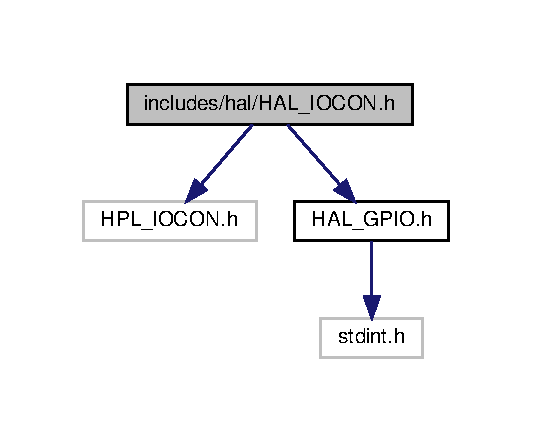
\includegraphics[width=350pt]{d2/ddf/HAL__IOCON_8h__incl}
\end{center}
\end{figure}
Gráfico de los archivos que directa o indirectamente incluyen a este archivo\+:\nopagebreak
\begin{figure}[H]
\begin{center}
\leavevmode
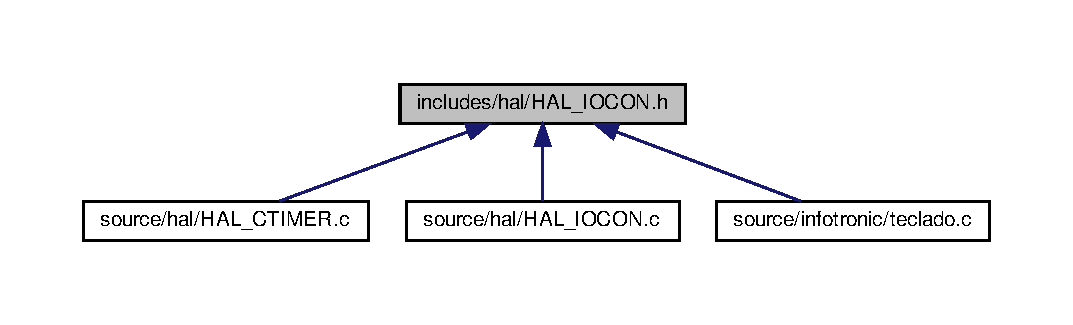
\includegraphics[width=350pt]{d7/de0/HAL__IOCON_8h__dep__incl}
\end{center}
\end{figure}
\subsection*{Estructuras de datos}
\begin{DoxyCompactItemize}
\item 
struct \hyperlink{HAL__IOCON_8h_dc/df0/structhal__iocon__config__t}{hal\+\_\+iocon\+\_\+config\+\_\+t}
\end{DoxyCompactItemize}
\subsection*{Enumeraciones}
\begin{DoxyCompactItemize}
\item 
\mbox{\Hypertarget{HAL__IOCON_8h_a63ecccb192eecfde5513839ac2a69431}\label{HAL__IOCON_8h_a63ecccb192eecfde5513839ac2a69431}} 
enum {\bfseries hal\+\_\+iocon\+\_\+pull\+\_\+mode\+\_\+en} \{ {\bfseries H\+A\+L\+\_\+\+I\+O\+C\+O\+N\+\_\+\+P\+U\+L\+L\+\_\+\+N\+O\+NE} = 0, 
{\bfseries H\+A\+L\+\_\+\+I\+O\+C\+O\+N\+\_\+\+P\+U\+L\+L\+\_\+\+D\+O\+WN}, 
{\bfseries H\+A\+L\+\_\+\+I\+O\+C\+O\+N\+\_\+\+P\+U\+L\+L\+\_\+\+UP}, 
{\bfseries H\+A\+L\+\_\+\+I\+O\+C\+O\+N\+\_\+\+P\+U\+L\+L\+\_\+\+R\+E\+P\+E\+A\+T\+ER}
 \}
\item 
\mbox{\Hypertarget{HAL__IOCON_8h_a41306d2caced0b5f04e58a44d48dfd09}\label{HAL__IOCON_8h_a41306d2caced0b5f04e58a44d48dfd09}} 
enum {\bfseries hal\+\_\+iocon\+\_\+sample\+\_\+mode\+\_\+en} \{ {\bfseries H\+A\+L\+\_\+\+I\+O\+C\+O\+N\+\_\+\+S\+A\+M\+P\+L\+E\+\_\+\+M\+O\+D\+E\+\_\+\+B\+Y\+P\+A\+SS} = 0, 
{\bfseries H\+A\+L\+\_\+\+I\+O\+C\+O\+N\+\_\+\+S\+A\+M\+P\+L\+E\+\_\+\+M\+O\+D\+E\+\_\+1\+\_\+\+C\+L\+O\+CK}, 
{\bfseries H\+A\+L\+\_\+\+I\+O\+C\+O\+N\+\_\+\+S\+A\+M\+P\+L\+E\+\_\+\+M\+O\+D\+E\+\_\+2\+\_\+\+C\+L\+O\+CK}, 
{\bfseries H\+A\+L\+\_\+\+I\+O\+C\+O\+N\+\_\+\+S\+A\+M\+P\+L\+E\+\_\+\+M\+O\+D\+E\+\_\+3\+\_\+\+C\+L\+O\+CK}
 \}
\item 
\mbox{\Hypertarget{HAL__IOCON_8h_a0b6a60b068de7a0cb787eaa62055acae}\label{HAL__IOCON_8h_a0b6a60b068de7a0cb787eaa62055acae}} 
enum {\bfseries hal\+\_\+iocon\+\_\+clk\+\_\+sel\+\_\+en} \{ \newline
{\bfseries H\+A\+L\+\_\+\+I\+O\+C\+O\+N\+\_\+\+C\+L\+K\+\_\+\+D\+I\+V\+\_\+0} = 0, 
{\bfseries H\+A\+L\+\_\+\+I\+O\+C\+O\+N\+\_\+\+C\+L\+K\+\_\+\+D\+I\+V\+\_\+1}, 
{\bfseries H\+A\+L\+\_\+\+I\+O\+C\+O\+N\+\_\+\+C\+L\+K\+\_\+\+D\+I\+V\+\_\+2}, 
{\bfseries H\+A\+L\+\_\+\+I\+O\+C\+O\+N\+\_\+\+C\+L\+K\+\_\+\+D\+I\+V\+\_\+3}, 
\newline
{\bfseries H\+A\+L\+\_\+\+I\+O\+C\+O\+N\+\_\+\+C\+L\+K\+\_\+\+D\+I\+V\+\_\+4}, 
{\bfseries H\+A\+L\+\_\+\+I\+O\+C\+O\+N\+\_\+\+C\+L\+K\+\_\+\+D\+I\+V\+\_\+5}, 
{\bfseries H\+A\+L\+\_\+\+I\+O\+C\+O\+N\+\_\+\+C\+L\+K\+\_\+\+D\+I\+V\+\_\+6}
 \}
\item 
\mbox{\Hypertarget{HAL__IOCON_8h_ac5adeae1bf96c489da06d9447800e9c0}\label{HAL__IOCON_8h_ac5adeae1bf96c489da06d9447800e9c0}} 
enum {\bfseries hal\+\_\+iocon\+\_\+iic\+\_\+mode\+\_\+en} \{ {\bfseries H\+A\+L\+\_\+\+I\+O\+C\+O\+N\+\_\+\+I\+I\+C\+\_\+\+M\+O\+D\+E\+\_\+\+S\+T\+A\+N\+D\+A\+RD} = 0, 
{\bfseries H\+A\+L\+\_\+\+I\+O\+C\+O\+N\+\_\+\+I\+I\+C\+\_\+\+M\+O\+D\+E\+\_\+\+G\+P\+IO}, 
{\bfseries H\+A\+L\+\_\+\+I\+O\+C\+O\+N\+\_\+\+I\+I\+C\+\_\+\+M\+O\+D\+E\+\_\+\+F\+A\+S\+T\+\_\+\+M\+O\+DE}
 \}
\end{DoxyCompactItemize}
\subsection*{Funciones}
\begin{DoxyCompactItemize}
\item 
void \hyperlink{HAL__IOCON_8h_af7f22380a268cadbc2928e6a5bb18b88}{hal\+\_\+iocon\+\_\+config\+\_\+io} (hal\+\_\+gpio\+\_\+portpin\+\_\+en portpin, const \hyperlink{HAL__IOCON_8h_dc/df0/structhal__iocon__config__t}{hal\+\_\+iocon\+\_\+config\+\_\+t} $\ast$config)
\begin{DoxyCompactList}\small\item\em Configuracion de un pin. \end{DoxyCompactList}\end{DoxyCompactItemize}


\subsection{Descripción detallada}
Declaraciones a nivel de aplicacion del periferico I\+O\+C\+ON (L\+P\+C845) 

\begin{DoxyAuthor}{Autor}
Augusto Santini 
\end{DoxyAuthor}
\begin{DoxyDate}{Fecha}
3/2020 
\end{DoxyDate}
\begin{DoxyVersion}{Versión}
1.\+0 
\end{DoxyVersion}


\subsection{Documentación de las estructuras de datos}
\index{hal\+\_\+iocon\+\_\+config\+\_\+t@{hal\+\_\+iocon\+\_\+config\+\_\+t}}\label{structhal__iocon__config__t}
\Hypertarget{HAL__IOCON_8h_structhal__iocon__config__t}
\subsubsection{struct hal\+\_\+iocon\+\_\+config\+\_\+t}
\begin{DoxyFields}{Campos de datos}
\mbox{\Hypertarget{HAL__IOCON_8h_aa22f2560bc78d947824f4cfe5124eda7}\label{HAL__IOCON_8h_aa22f2560bc78d947824f4cfe5124eda7}} 
hal\_iocon\_pull\_mode\_en&
pull\_mode&
\\
\hline

\mbox{\Hypertarget{HAL__IOCON_8h_a2e9773d4803e8e976a13292cd2ad0c7a}\label{HAL__IOCON_8h_a2e9773d4803e8e976a13292cd2ad0c7a}} 
uint8\_t&
hysteresis&
\\
\hline

\mbox{\Hypertarget{HAL__IOCON_8h_a72cc41e5bf068e3e77e04797ad0927da}\label{HAL__IOCON_8h_a72cc41e5bf068e3e77e04797ad0927da}} 
uint8\_t&
invert\_input&
\\
\hline

\mbox{\Hypertarget{HAL__IOCON_8h_a1e960a1499ff856953454bb4bae0cb79}\label{HAL__IOCON_8h_a1e960a1499ff856953454bb4bae0cb79}} 
uint8\_t&
open\_drain&
\\
\hline

\mbox{\Hypertarget{HAL__IOCON_8h_a2bd76ef14f9b9048b414adbcd623d390}\label{HAL__IOCON_8h_a2bd76ef14f9b9048b414adbcd623d390}} 
hal\_iocon\_sample\_mode\_en&
sample\_mode&
\\
\hline

\mbox{\Hypertarget{HAL__IOCON_8h_a088a30034e6d3ce3ae44f171eebf8679}\label{HAL__IOCON_8h_a088a30034e6d3ce3ae44f171eebf8679}} 
hal\_iocon\_clk\_sel\_en&
clk\_sel&
\\
\hline

\mbox{\Hypertarget{HAL__IOCON_8h_a9444f75dcd09dd998209e13f4df83b11}\label{HAL__IOCON_8h_a9444f75dcd09dd998209e13f4df83b11}} 
uint8\_t&
dac\_mode&
\\
\hline

\mbox{\Hypertarget{HAL__IOCON_8h_ab637420afee560be573a20f19fbb0e1a}\label{HAL__IOCON_8h_ab637420afee560be573a20f19fbb0e1a}} 
hal\_iocon\_iic\_mode\_en&
iic\_mode&
\\
\hline

\end{DoxyFields}


\subsection{Documentación de las funciones}
\mbox{\Hypertarget{HAL__IOCON_8h_af7f22380a268cadbc2928e6a5bb18b88}\label{HAL__IOCON_8h_af7f22380a268cadbc2928e6a5bb18b88}} 
\index{H\+A\+L\+\_\+\+I\+O\+C\+O\+N.\+h@{H\+A\+L\+\_\+\+I\+O\+C\+O\+N.\+h}!hal\+\_\+iocon\+\_\+config\+\_\+io@{hal\+\_\+iocon\+\_\+config\+\_\+io}}
\index{hal\+\_\+iocon\+\_\+config\+\_\+io@{hal\+\_\+iocon\+\_\+config\+\_\+io}!H\+A\+L\+\_\+\+I\+O\+C\+O\+N.\+h@{H\+A\+L\+\_\+\+I\+O\+C\+O\+N.\+h}}
\subsubsection{\texorpdfstring{hal\+\_\+iocon\+\_\+config\+\_\+io()}{hal\_iocon\_config\_io()}}
{\footnotesize\ttfamily void hal\+\_\+iocon\+\_\+config\+\_\+io (\begin{DoxyParamCaption}\item[{hal\+\_\+gpio\+\_\+portpin\+\_\+en}]{portpin,  }\item[{const \hyperlink{HAL__IOCON_8h_dc/df0/structhal__iocon__config__t}{hal\+\_\+iocon\+\_\+config\+\_\+t} $\ast$}]{config }\end{DoxyParamCaption})}



Configuracion de un pin. 


\begin{DoxyParams}[1]{Parámetros}
\mbox{\tt in}  & {\em portpin} & Puerto/pin a configurar \\
\hline
\mbox{\tt in}  & {\em pin\+\_\+config} & Puntero a estructura de configuracion del pin \\
\hline
\end{DoxyParams}

\hypertarget{HAL__PININT_8h}{}\doxysection{Referencia del Archivo includes/hal/\+H\+A\+L\+\_\+\+P\+I\+N\+I\+NT.h}
\label{HAL__PININT_8h}\index{includes/hal/HAL\_PININT.h@{includes/hal/HAL\_PININT.h}}


Declaraciones a nivel de aplicacion del periferico P\+I\+N\+I\+NT (L\+P\+C845)  


{\ttfamily \#include $<$stdint.\+h$>$}\newline
{\ttfamily \#include $<$H\+A\+L\+\_\+\+G\+P\+I\+O.\+h$>$}\newline
Dependencia gráfica adjunta para H\+A\+L\+\_\+\+P\+I\+N\+I\+N\+T.\+h\+:\nopagebreak
\begin{figure}[H]
\begin{center}
\leavevmode
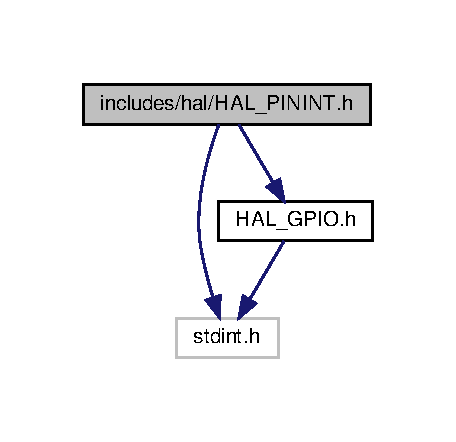
\includegraphics[width=219pt]{HAL__PININT_8h__incl}
\end{center}
\end{figure}
\doxysubsection*{Estructuras de datos}
\begin{DoxyCompactItemize}
\item 
struct \mbox{\hyperlink{structhal__pinint__config__t}{hal\+\_\+pinint\+\_\+config\+\_\+t}}
\end{DoxyCompactItemize}
\doxysubsection*{Enumeraciones}
\begin{DoxyCompactItemize}
\item 
\mbox{\Hypertarget{HAL__PININT_8h_a4ae16eed9cc4c0afbb4b43d8ff47c87c}\label{HAL__PININT_8h_a4ae16eed9cc4c0afbb4b43d8ff47c87c}} 
enum {\bfseries hal\+\_\+pinint\+\_\+channel\+\_\+en} \{ \newline
{\bfseries H\+A\+L\+\_\+\+P\+I\+N\+I\+N\+T\+\_\+\+C\+H\+A\+N\+N\+E\+L\+\_\+0} = 0, 
{\bfseries H\+A\+L\+\_\+\+P\+I\+N\+I\+N\+T\+\_\+\+C\+H\+A\+N\+N\+E\+L\+\_\+1}, 
{\bfseries H\+A\+L\+\_\+\+P\+I\+N\+I\+N\+T\+\_\+\+C\+H\+A\+N\+N\+E\+L\+\_\+2}, 
{\bfseries H\+A\+L\+\_\+\+P\+I\+N\+I\+N\+T\+\_\+\+C\+H\+A\+N\+N\+E\+L\+\_\+3}, 
\newline
{\bfseries H\+A\+L\+\_\+\+P\+I\+N\+I\+N\+T\+\_\+\+C\+H\+A\+N\+N\+E\+L\+\_\+4}, 
{\bfseries H\+A\+L\+\_\+\+P\+I\+N\+I\+N\+T\+\_\+\+C\+H\+A\+N\+N\+E\+L\+\_\+5}, 
{\bfseries H\+A\+L\+\_\+\+P\+I\+N\+I\+N\+T\+\_\+\+C\+H\+A\+N\+N\+E\+L\+\_\+6}, 
{\bfseries H\+A\+L\+\_\+\+P\+I\+N\+I\+N\+T\+\_\+\+C\+H\+A\+N\+N\+E\+L\+\_\+7}
 \}
\item 
\mbox{\Hypertarget{HAL__PININT_8h_a5a9a36a223fb9ec5c125d0acdc1c8ba3}\label{HAL__PININT_8h_a5a9a36a223fb9ec5c125d0acdc1c8ba3}} 
enum {\bfseries hal\+\_\+pinint\+\_\+interrupt\+\_\+mode\+\_\+en} \{ {\bfseries H\+A\+L\+\_\+\+P\+I\+N\+I\+N\+T\+\_\+\+I\+N\+T\+E\+R\+R\+U\+P\+T\+\_\+\+M\+O\+D\+E\+\_\+\+E\+D\+GE} = 0, 
{\bfseries H\+A\+L\+\_\+\+P\+I\+N\+I\+N\+T\+\_\+\+I\+N\+T\+E\+R\+R\+U\+P\+T\+\_\+\+M\+O\+D\+E\+\_\+\+L\+E\+V\+EL}
 \}
\item 
\mbox{\Hypertarget{HAL__PININT_8h_af9e709e533d1b2848c2b7a56c70e6bcb}\label{HAL__PININT_8h_af9e709e533d1b2848c2b7a56c70e6bcb}} 
enum {\bfseries hal\+\_\+pinint\+\_\+level\+\_\+int\+\_\+en} \{ {\bfseries H\+A\+L\+\_\+\+P\+I\+N\+I\+N\+T\+\_\+\+L\+E\+V\+E\+L\+\_\+\+I\+N\+T\+\_\+\+H\+I\+GH} = 0, 
{\bfseries H\+A\+L\+\_\+\+P\+I\+N\+I\+N\+T\+\_\+\+L\+E\+V\+E\+L\+\_\+\+I\+N\+T\+\_\+\+L\+OW}
 \}
\end{DoxyCompactItemize}
\doxysubsection*{Funciones}
\begin{DoxyCompactItemize}
\item 
\mbox{\Hypertarget{HAL__PININT_8h_aa0cbe5b8bc592e4731d28667e5dfc30f}\label{HAL__PININT_8h_aa0cbe5b8bc592e4731d28667e5dfc30f}} 
void \mbox{\hyperlink{HAL__PININT_8h_aa0cbe5b8bc592e4731d28667e5dfc30f}{hal\+\_\+pinint\+\_\+init}} (void)
\begin{DoxyCompactList}\small\item\em Inicializacion del modulo. \end{DoxyCompactList}\item 
void \mbox{\hyperlink{HAL__PININT_8h_a4b7e39b58f03c04edd28846ead64cbd7}{hal\+\_\+pinint\+\_\+configure\+\_\+pin\+\_\+interrupt}} (const \mbox{\hyperlink{structhal__pinint__config__t}{hal\+\_\+pinint\+\_\+config\+\_\+t}} $\ast$config)
\begin{DoxyCompactList}\small\item\em Configurar interrupciones de pin. \end{DoxyCompactList}\item 
void \mbox{\hyperlink{HAL__PININT_8h_a201dfb9bbe81b35792f5f335b9e7dc11}{hal\+\_\+pinint\+\_\+register\+\_\+callback}} (hal\+\_\+pinint\+\_\+channel\+\_\+en channel, void($\ast$new\+\_\+callback)(void))
\begin{DoxyCompactList}\small\item\em Registrar callback a llamar en interrupcion de P\+I\+N\+I\+N\+Tn. \end{DoxyCompactList}\end{DoxyCompactItemize}


\doxysubsection{Descripción detallada}
Declaraciones a nivel de aplicacion del periferico P\+I\+N\+I\+NT (L\+P\+C845) 

\begin{DoxyAuthor}{Autor}
Augusto Santini 
\end{DoxyAuthor}
\begin{DoxyDate}{Fecha}
3/2020 
\end{DoxyDate}
\begin{DoxyVersion}{Versión}
1.\+0 
\end{DoxyVersion}


\doxysubsection{Documentación de las funciones}
\mbox{\Hypertarget{HAL__PININT_8h_a4b7e39b58f03c04edd28846ead64cbd7}\label{HAL__PININT_8h_a4b7e39b58f03c04edd28846ead64cbd7}} 
\index{HAL\_PININT.h@{HAL\_PININT.h}!hal\_pinint\_configure\_pin\_interrupt@{hal\_pinint\_configure\_pin\_interrupt}}
\index{hal\_pinint\_configure\_pin\_interrupt@{hal\_pinint\_configure\_pin\_interrupt}!HAL\_PININT.h@{HAL\_PININT.h}}
\doxysubsubsection{\texorpdfstring{hal\_pinint\_configure\_pin\_interrupt()}{hal\_pinint\_configure\_pin\_interrupt()}}
{\footnotesize\ttfamily void hal\+\_\+pinint\+\_\+configure\+\_\+pin\+\_\+interrupt (\begin{DoxyParamCaption}\item[{const \mbox{\hyperlink{structhal__pinint__config__t}{hal\+\_\+pinint\+\_\+config\+\_\+t}} $\ast$}]{config }\end{DoxyParamCaption})}



Configurar interrupciones de pin. 


\begin{DoxyParams}[1]{Parámetros}
\mbox{\texttt{ in}}  & {\em config} & Configuracion de interrupciones de pin \\
\hline
\end{DoxyParams}
\mbox{\Hypertarget{HAL__PININT_8h_a201dfb9bbe81b35792f5f335b9e7dc11}\label{HAL__PININT_8h_a201dfb9bbe81b35792f5f335b9e7dc11}} 
\index{HAL\_PININT.h@{HAL\_PININT.h}!hal\_pinint\_register\_callback@{hal\_pinint\_register\_callback}}
\index{hal\_pinint\_register\_callback@{hal\_pinint\_register\_callback}!HAL\_PININT.h@{HAL\_PININT.h}}
\doxysubsubsection{\texorpdfstring{hal\_pinint\_register\_callback()}{hal\_pinint\_register\_callback()}}
{\footnotesize\ttfamily void hal\+\_\+pinint\+\_\+register\+\_\+callback (\begin{DoxyParamCaption}\item[{hal\+\_\+pinint\+\_\+channel\+\_\+en}]{channel,  }\item[{void($\ast$)(void)}]{new\+\_\+callback }\end{DoxyParamCaption})}



Registrar callback a llamar en interrupcion de P\+I\+N\+I\+N\+Tn. 


\begin{DoxyParams}[1]{Parámetros}
\mbox{\texttt{ in}}  & {\em channel} & Canal al cual registrar el callback \\
\hline
\mbox{\texttt{ in}}  & {\em new\+\_\+callback} & Puntero a funcion a ejecutar \\
\hline
\end{DoxyParams}

\hypertarget{HAL__SPI_8h}{}\section{Referencia del Archivo includes/hal/\+H\+A\+L\+\_\+\+S\+PI.h}
\label{HAL__SPI_8h}\index{includes/hal/\+H\+A\+L\+\_\+\+S\+P\+I.\+h@{includes/hal/\+H\+A\+L\+\_\+\+S\+P\+I.\+h}}


Declaraciones a nivel de aplicacion del periferico S\+PI (L\+P\+C845)  


{\ttfamily \#include $<$stdint.\+h$>$}\newline
{\ttfamily \#include $<$H\+A\+L\+\_\+\+S\+Y\+S\+C\+O\+N.\+h$>$}\newline
{\ttfamily \#include $<$H\+A\+L\+\_\+\+G\+P\+I\+O.\+h$>$}\newline
Dependencia gráfica adjunta para H\+A\+L\+\_\+\+S\+P\+I.\+h\+:
\nopagebreak
\begin{figure}[H]
\begin{center}
\leavevmode
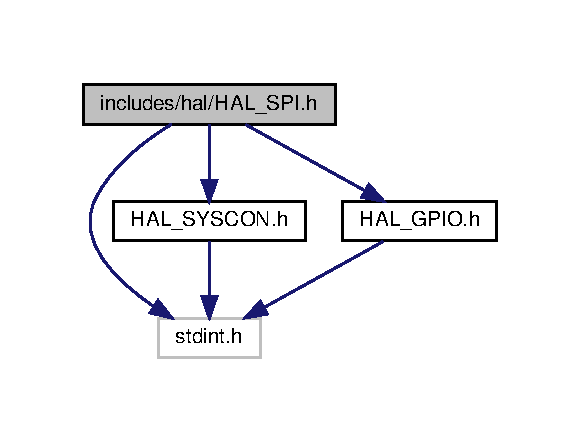
\includegraphics[width=279pt]{HAL__SPI_8h__incl}
\end{center}
\end{figure}
\subsection*{Estructuras de datos}
\begin{DoxyCompactItemize}
\item 
struct \hyperlink{structhal__spi__master__mode__config__t}{hal\+\_\+spi\+\_\+master\+\_\+mode\+\_\+config\+\_\+t}
\item 
struct \hyperlink{HAL__SPI_8h_structhal__spi__master__mode__tx__config__t}{hal\+\_\+spi\+\_\+master\+\_\+mode\+\_\+tx\+\_\+config\+\_\+t}
\item 
struct \hyperlink{HAL__SPI_8h_structhal__spi__master__mode__tx__data__t}{hal\+\_\+spi\+\_\+master\+\_\+mode\+\_\+tx\+\_\+data\+\_\+t}
\end{DoxyCompactItemize}
\subsection*{defines}
\begin{DoxyCompactItemize}
\item 
\mbox{\Hypertarget{HAL__SPI_8h_aa155c3ad4568672fbec24698f9e267ad}\label{HAL__SPI_8h_aa155c3ad4568672fbec24698f9e267ad}} 
\#define {\bfseries H\+A\+L\+\_\+\+S\+P\+I\+\_\+\+D\+U\+M\+M\+Y\+\_\+\+B\+Y\+TE}~(0x\+F\+F)
\end{DoxyCompactItemize}
\subsection*{Enumeraciones}
\begin{DoxyCompactItemize}
\item 
\mbox{\Hypertarget{HAL__SPI_8h_af0531d47c7a0508e49c239b8ac94eecb}\label{HAL__SPI_8h_af0531d47c7a0508e49c239b8ac94eecb}} 
enum {\bfseries hal\+\_\+spi\+\_\+sel\+\_\+en} \{ {\bfseries H\+A\+L\+\_\+\+S\+P\+I\+\_\+0} = 0, 
{\bfseries H\+A\+L\+\_\+\+S\+P\+I\+\_\+1}
 \}
\item 
\mbox{\Hypertarget{HAL__SPI_8h_a227108083b750e225901d1e2ee8ba2c1}\label{HAL__SPI_8h_a227108083b750e225901d1e2ee8ba2c1}} 
enum {\bfseries hal\+\_\+spi\+\_\+data\+\_\+length\+\_\+en} \{ \newline
{\bfseries H\+A\+L\+\_\+\+S\+P\+I\+\_\+\+D\+A\+T\+A\+\_\+\+L\+E\+N\+G\+T\+H\+\_\+1\+\_\+\+B\+IT} = 0, 
{\bfseries H\+A\+L\+\_\+\+S\+P\+I\+\_\+\+D\+A\+T\+A\+\_\+\+L\+E\+N\+G\+T\+H\+\_\+2\+\_\+\+B\+IT}, 
{\bfseries H\+A\+L\+\_\+\+S\+P\+I\+\_\+\+D\+A\+T\+A\+\_\+\+L\+E\+N\+G\+T\+H\+\_\+3\+\_\+\+B\+IT}, 
{\bfseries H\+A\+L\+\_\+\+S\+P\+I\+\_\+\+D\+A\+T\+A\+\_\+\+L\+E\+N\+G\+T\+H\+\_\+4\+\_\+\+B\+IT}, 
\newline
{\bfseries H\+A\+L\+\_\+\+S\+P\+I\+\_\+\+D\+A\+T\+A\+\_\+\+L\+E\+N\+G\+T\+H\+\_\+5\+\_\+\+B\+IT}, 
{\bfseries H\+A\+L\+\_\+\+S\+P\+I\+\_\+\+D\+A\+T\+A\+\_\+\+L\+E\+N\+G\+T\+H\+\_\+6\+\_\+\+B\+IT}, 
{\bfseries H\+A\+L\+\_\+\+S\+P\+I\+\_\+\+D\+A\+T\+A\+\_\+\+L\+E\+N\+G\+T\+H\+\_\+7\+\_\+\+B\+IT}, 
{\bfseries H\+A\+L\+\_\+\+S\+P\+I\+\_\+\+D\+A\+T\+A\+\_\+\+L\+E\+N\+G\+T\+H\+\_\+8\+\_\+\+B\+IT}, 
\newline
{\bfseries H\+A\+L\+\_\+\+S\+P\+I\+\_\+\+D\+A\+T\+A\+\_\+\+L\+E\+N\+G\+T\+H\+\_\+9\+\_\+\+B\+IT}, 
{\bfseries H\+A\+L\+\_\+\+S\+P\+I\+\_\+\+D\+A\+T\+A\+\_\+\+L\+E\+N\+G\+T\+H\+\_\+10\+\_\+\+B\+IT}, 
{\bfseries H\+A\+L\+\_\+\+S\+P\+I\+\_\+\+D\+A\+T\+A\+\_\+\+L\+E\+N\+G\+T\+H\+\_\+11\+\_\+\+B\+IT}, 
{\bfseries H\+A\+L\+\_\+\+S\+P\+I\+\_\+\+D\+A\+T\+A\+\_\+\+L\+E\+N\+G\+T\+H\+\_\+12\+\_\+\+B\+IT}, 
\newline
{\bfseries H\+A\+L\+\_\+\+S\+P\+I\+\_\+\+D\+A\+T\+A\+\_\+\+L\+E\+N\+G\+T\+H\+\_\+13\+\_\+\+B\+IT}, 
{\bfseries H\+A\+L\+\_\+\+S\+P\+I\+\_\+\+D\+A\+T\+A\+\_\+\+L\+E\+N\+G\+T\+H\+\_\+14\+\_\+\+B\+IT}, 
{\bfseries H\+A\+L\+\_\+\+S\+P\+I\+\_\+\+D\+A\+T\+A\+\_\+\+L\+E\+N\+G\+T\+H\+\_\+15\+\_\+\+B\+IT}, 
{\bfseries H\+A\+L\+\_\+\+S\+P\+I\+\_\+\+D\+A\+T\+A\+\_\+\+L\+E\+N\+G\+T\+H\+\_\+16\+\_\+\+B\+IT}
 \}
\item 
\mbox{\Hypertarget{HAL__SPI_8h_abe5c2177f6baea2b1eb394325a11f8d3}\label{HAL__SPI_8h_abe5c2177f6baea2b1eb394325a11f8d3}} 
enum {\bfseries hal\+\_\+spi\+\_\+clock\+\_\+mode\+\_\+en} \{ {\bfseries H\+A\+L\+\_\+\+S\+P\+I\+\_\+\+C\+L\+O\+C\+K\+\_\+\+M\+O\+D\+E\+\_\+0} = 0, 
{\bfseries H\+A\+L\+\_\+\+S\+P\+I\+\_\+\+C\+L\+O\+C\+K\+\_\+\+M\+O\+D\+E\+\_\+1}, 
{\bfseries H\+A\+L\+\_\+\+S\+P\+I\+\_\+\+C\+L\+O\+C\+K\+\_\+\+M\+O\+D\+E\+\_\+2}, 
{\bfseries H\+A\+L\+\_\+\+S\+P\+I\+\_\+\+C\+L\+O\+C\+K\+\_\+\+M\+O\+D\+E\+\_\+3}
 \}
\item 
\mbox{\Hypertarget{HAL__SPI_8h_ae4b694f0781b20b8c818d568fe39f20f}\label{HAL__SPI_8h_ae4b694f0781b20b8c818d568fe39f20f}} 
enum {\bfseries hal\+\_\+spi\+\_\+ssel\+\_\+polarity\+\_\+en} \{ {\bfseries H\+A\+L\+\_\+\+S\+P\+I\+\_\+\+S\+S\+E\+L\+\_\+\+P\+O\+L\+A\+R\+I\+T\+Y\+\_\+\+L\+OW} = 0, 
{\bfseries H\+A\+L\+\_\+\+S\+P\+I\+\_\+\+S\+S\+E\+L\+\_\+\+P\+O\+L\+A\+R\+I\+T\+Y\+\_\+\+H\+I\+GH}
 \}
\item 
\mbox{\Hypertarget{HAL__SPI_8h_ae079f1e93eaa69c19c037409e48cabaa}\label{HAL__SPI_8h_ae079f1e93eaa69c19c037409e48cabaa}} 
enum {\bfseries hal\+\_\+spi\+\_\+ssel\+\_\+sel\+\_\+en} \{ \newline
{\bfseries H\+A\+L\+\_\+\+S\+P\+I\+\_\+\+S\+S\+E\+L\+\_\+\+S\+E\+L\+E\+C\+T\+I\+O\+N\+\_\+0} = 0, 
{\bfseries H\+A\+L\+\_\+\+S\+P\+I\+\_\+\+S\+S\+E\+L\+\_\+\+S\+E\+L\+E\+C\+T\+I\+O\+N\+\_\+1}, 
{\bfseries H\+A\+L\+\_\+\+S\+P\+I\+\_\+\+S\+S\+E\+L\+\_\+\+S\+E\+L\+E\+C\+T\+I\+O\+N\+\_\+2}, 
{\bfseries H\+A\+L\+\_\+\+S\+P\+I\+\_\+\+S\+S\+E\+L\+\_\+\+S\+E\+L\+E\+C\+T\+I\+O\+N\+\_\+3}, 
\newline
{\bfseries H\+A\+L\+\_\+\+S\+P\+I\+\_\+\+S\+S\+E\+L\+\_\+\+S\+E\+L\+E\+C\+T\+I\+O\+N\+\_\+\+O\+T\+H\+ER}
 \}
\end{DoxyCompactItemize}
\subsection*{Funciones}
\begin{DoxyCompactItemize}
\item 
void \hyperlink{HAL__SPI_8h_a9babc814c41f2d8714551fc9af81d346}{hal\+\_\+spi\+\_\+master\+\_\+mode\+\_\+init} (hal\+\_\+spi\+\_\+sel\+\_\+en inst, const \hyperlink{structhal__spi__master__mode__config__t}{hal\+\_\+spi\+\_\+master\+\_\+mode\+\_\+config\+\_\+t} $\ast$config)
\begin{DoxyCompactList}\small\item\em Inicializar S\+PI en modo master. \end{DoxyCompactList}\item 
uint16\+\_\+t \hyperlink{HAL__SPI_8h_a6ca16392e2331ab9db9d97f3a6358346}{hal\+\_\+spi\+\_\+master\+\_\+mode\+\_\+rx\+\_\+data} (hal\+\_\+spi\+\_\+sel\+\_\+en inst)
\begin{DoxyCompactList}\small\item\em Leer el dato recibido. \end{DoxyCompactList}\item 
void \hyperlink{HAL__SPI_8h_a11b672c8dcef79e8784497b23f1618b7}{hal\+\_\+spi\+\_\+master\+\_\+mode\+\_\+config\+\_\+tx} (hal\+\_\+spi\+\_\+sel\+\_\+en inst, const \hyperlink{HAL__SPI_8h_structhal__spi__master__mode__tx__config__t}{hal\+\_\+spi\+\_\+master\+\_\+mode\+\_\+tx\+\_\+config\+\_\+t} $\ast$config)
\begin{DoxyCompactList}\small\item\em Configurar la transmision. \end{DoxyCompactList}\item 
void \hyperlink{HAL__SPI_8h_ad7cfe819f562f90c6bb07e2577699d86}{hal\+\_\+spi\+\_\+master\+\_\+mode\+\_\+tx\+\_\+data} (hal\+\_\+spi\+\_\+sel\+\_\+en inst, const \hyperlink{HAL__SPI_8h_structhal__spi__master__mode__tx__data__t}{hal\+\_\+spi\+\_\+master\+\_\+mode\+\_\+tx\+\_\+data\+\_\+t} $\ast$data)
\begin{DoxyCompactList}\small\item\em Transmitir dato. \end{DoxyCompactList}\item 
void \hyperlink{HAL__SPI_8h_a5bbc56bb8e86b9b077822fab5297e513}{hal\+\_\+spi\+\_\+master\+\_\+mode\+\_\+register\+\_\+tx\+\_\+callback} (hal\+\_\+spi\+\_\+sel\+\_\+en inst, void($\ast$new\+\_\+callback)(void))
\begin{DoxyCompactList}\small\item\em Actualizar callback en T\+X\+R\+DY. \end{DoxyCompactList}\item 
void \hyperlink{HAL__SPI_8h_a363e7e3be50a625bd8fe6a748c473027}{hal\+\_\+spi\+\_\+master\+\_\+mode\+\_\+register\+\_\+rx\+\_\+callback} (hal\+\_\+spi\+\_\+sel\+\_\+en inst, void($\ast$new\+\_\+callback)(void))
\begin{DoxyCompactList}\small\item\em Actualizar callback en R\+X\+R\+DY. \end{DoxyCompactList}\end{DoxyCompactItemize}


\subsection{Descripción detallada}
Declaraciones a nivel de aplicacion del periferico S\+PI (L\+P\+C845) 

\begin{DoxyAuthor}{Autor}
Augusto Santini 
\end{DoxyAuthor}
\begin{DoxyDate}{Fecha}
3/2020 
\end{DoxyDate}
\begin{DoxyVersion}{Versión}
1.\+0 
\end{DoxyVersion}


\subsection{Documentación de las estructuras de datos}
\index{hal\+\_\+spi\+\_\+master\+\_\+mode\+\_\+tx\+\_\+config\+\_\+t@{hal\+\_\+spi\+\_\+master\+\_\+mode\+\_\+tx\+\_\+config\+\_\+t}}\label{structhal__spi__master__mode__tx__config__t}
\Hypertarget{HAL__SPI_8h_structhal__spi__master__mode__tx__config__t}
\subsubsection{struct hal\+\_\+spi\+\_\+master\+\_\+mode\+\_\+tx\+\_\+config\+\_\+t}
\begin{DoxyFields}{Campos de datos}
\mbox{\Hypertarget{HAL__SPI_8h_af409a6b3ff876d386c8d9b38f05e633c}\label{HAL__SPI_8h_af409a6b3ff876d386c8d9b38f05e633c}} 
hal\_spi\_clock\_mode\_en&
clock\_mode&
\\
\hline

\mbox{\Hypertarget{HAL__SPI_8h_a3f6dc062eedd7440d333341c9fa187fc}\label{HAL__SPI_8h_a3f6dc062eedd7440d333341c9fa187fc}} 
uint16\_t&
clock\_div&
\\
\hline

\end{DoxyFields}
\index{hal\+\_\+spi\+\_\+master\+\_\+mode\+\_\+tx\+\_\+data\+\_\+t@{hal\+\_\+spi\+\_\+master\+\_\+mode\+\_\+tx\+\_\+data\+\_\+t}}\label{structhal__spi__master__mode__tx__data__t}
\Hypertarget{HAL__SPI_8h_structhal__spi__master__mode__tx__data__t}
\subsubsection{struct hal\+\_\+spi\+\_\+master\+\_\+mode\+\_\+tx\+\_\+data\+\_\+t}
\begin{DoxyFields}{Campos de datos}
\mbox{\Hypertarget{HAL__SPI_8h_ace5d9edd50ae7a04c202ce1aa9ffc9d1}\label{HAL__SPI_8h_ace5d9edd50ae7a04c202ce1aa9ffc9d1}} 
uint32\_t&
data: 16&
\\
\hline

\mbox{\Hypertarget{HAL__SPI_8h_aaab3fc186c57a63900f5993863c07c4a}\label{HAL__SPI_8h_aaab3fc186c57a63900f5993863c07c4a}} 
uint32\_t&
ssel0\_n: 1&
\\
\hline

\mbox{\Hypertarget{HAL__SPI_8h_a48d1d2904f75bc7168ff179a3aeb104d}\label{HAL__SPI_8h_a48d1d2904f75bc7168ff179a3aeb104d}} 
uint32\_t&
ssel1\_n: 1&
\\
\hline

\mbox{\Hypertarget{HAL__SPI_8h_a6f213524ceb263d64b63185d52638901}\label{HAL__SPI_8h_a6f213524ceb263d64b63185d52638901}} 
uint32\_t&
ssel2\_n: 1&
\\
\hline

\mbox{\Hypertarget{HAL__SPI_8h_adc9f4bc3389a51df667606fc05ab7b20}\label{HAL__SPI_8h_adc9f4bc3389a51df667606fc05ab7b20}} 
uint32\_t&
ssel3\_n: 1&
\\
\hline

\mbox{\Hypertarget{HAL__SPI_8h_af150436bf862f82b00a2e7b759684a74}\label{HAL__SPI_8h_af150436bf862f82b00a2e7b759684a74}} 
uint32\_t&
eot: 1&
\\
\hline

\mbox{\Hypertarget{HAL__SPI_8h_a01f721e64eb8c6d026cbbdf42e85da2b}\label{HAL__SPI_8h_a01f721e64eb8c6d026cbbdf42e85da2b}} 
uint32\_t&
eof: 1&
\\
\hline

\mbox{\Hypertarget{HAL__SPI_8h_a0ea6f255ed33e8bc7af80de3dec62e65}\label{HAL__SPI_8h_a0ea6f255ed33e8bc7af80de3dec62e65}} 
uint32\_t&
rxignore: 1&
\\
\hline

\mbox{\Hypertarget{HAL__SPI_8h_a34120f9ce21c6560bd05d5b0cbcf6b3c}\label{HAL__SPI_8h_a34120f9ce21c6560bd05d5b0cbcf6b3c}} 
uint32\_t&
\_\_pad0\_\_: 1&
\\
\hline

\mbox{\Hypertarget{HAL__SPI_8h_a63c569f0b77034323eb485a9c67d4956}\label{HAL__SPI_8h_a63c569f0b77034323eb485a9c67d4956}} 
uint32\_t&
data\_length: 4&
\\
\hline

\mbox{\Hypertarget{HAL__SPI_8h_a5374a84b23db0afe275be7797c8f74b0}\label{HAL__SPI_8h_a5374a84b23db0afe275be7797c8f74b0}} 
uint32\_t&
\_\_pad1\_\_: 4&
\\
\hline

\end{DoxyFields}


\subsection{Documentación de las funciones}
\mbox{\Hypertarget{HAL__SPI_8h_a9babc814c41f2d8714551fc9af81d346}\label{HAL__SPI_8h_a9babc814c41f2d8714551fc9af81d346}} 
\index{H\+A\+L\+\_\+\+S\+P\+I.\+h@{H\+A\+L\+\_\+\+S\+P\+I.\+h}!hal\+\_\+spi\+\_\+master\+\_\+mode\+\_\+init@{hal\+\_\+spi\+\_\+master\+\_\+mode\+\_\+init}}
\index{hal\+\_\+spi\+\_\+master\+\_\+mode\+\_\+init@{hal\+\_\+spi\+\_\+master\+\_\+mode\+\_\+init}!H\+A\+L\+\_\+\+S\+P\+I.\+h@{H\+A\+L\+\_\+\+S\+P\+I.\+h}}
\subsubsection{\texorpdfstring{hal\+\_\+spi\+\_\+master\+\_\+mode\+\_\+init()}{hal\_spi\_master\_mode\_init()}}
{\footnotesize\ttfamily void hal\+\_\+spi\+\_\+master\+\_\+mode\+\_\+init (\begin{DoxyParamCaption}\item[{hal\+\_\+spi\+\_\+sel\+\_\+en}]{inst,  }\item[{const \hyperlink{structhal__spi__master__mode__config__t}{hal\+\_\+spi\+\_\+master\+\_\+mode\+\_\+config\+\_\+t} $\ast$}]{config }\end{DoxyParamCaption})}



Inicializar S\+PI en modo master. 


\begin{DoxyParams}[1]{Parámetros}
\mbox{\tt in}  & {\em inst} & Instancia de S\+PI a inicializar \\
\hline
\mbox{\tt in}  & {\em config} & Configuracion deseada \\
\hline
\end{DoxyParams}
\mbox{\Hypertarget{HAL__SPI_8h_a6ca16392e2331ab9db9d97f3a6358346}\label{HAL__SPI_8h_a6ca16392e2331ab9db9d97f3a6358346}} 
\index{H\+A\+L\+\_\+\+S\+P\+I.\+h@{H\+A\+L\+\_\+\+S\+P\+I.\+h}!hal\+\_\+spi\+\_\+master\+\_\+mode\+\_\+rx\+\_\+data@{hal\+\_\+spi\+\_\+master\+\_\+mode\+\_\+rx\+\_\+data}}
\index{hal\+\_\+spi\+\_\+master\+\_\+mode\+\_\+rx\+\_\+data@{hal\+\_\+spi\+\_\+master\+\_\+mode\+\_\+rx\+\_\+data}!H\+A\+L\+\_\+\+S\+P\+I.\+h@{H\+A\+L\+\_\+\+S\+P\+I.\+h}}
\subsubsection{\texorpdfstring{hal\+\_\+spi\+\_\+master\+\_\+mode\+\_\+rx\+\_\+data()}{hal\_spi\_master\_mode\_rx\_data()}}
{\footnotesize\ttfamily uint16\+\_\+t hal\+\_\+spi\+\_\+master\+\_\+mode\+\_\+rx\+\_\+data (\begin{DoxyParamCaption}\item[{hal\+\_\+spi\+\_\+sel\+\_\+en}]{inst }\end{DoxyParamCaption})}



Leer el dato recibido. 


\begin{DoxyParams}[1]{Parámetros}
\mbox{\tt in}  & {\em inst} & Instancia a consultar \\
\hline
\end{DoxyParams}
\begin{DoxyReturn}{Devuelve}
Dato recibido 
\end{DoxyReturn}
\mbox{\Hypertarget{HAL__SPI_8h_a11b672c8dcef79e8784497b23f1618b7}\label{HAL__SPI_8h_a11b672c8dcef79e8784497b23f1618b7}} 
\index{H\+A\+L\+\_\+\+S\+P\+I.\+h@{H\+A\+L\+\_\+\+S\+P\+I.\+h}!hal\+\_\+spi\+\_\+master\+\_\+mode\+\_\+config\+\_\+tx@{hal\+\_\+spi\+\_\+master\+\_\+mode\+\_\+config\+\_\+tx}}
\index{hal\+\_\+spi\+\_\+master\+\_\+mode\+\_\+config\+\_\+tx@{hal\+\_\+spi\+\_\+master\+\_\+mode\+\_\+config\+\_\+tx}!H\+A\+L\+\_\+\+S\+P\+I.\+h@{H\+A\+L\+\_\+\+S\+P\+I.\+h}}
\subsubsection{\texorpdfstring{hal\+\_\+spi\+\_\+master\+\_\+mode\+\_\+config\+\_\+tx()}{hal\_spi\_master\_mode\_config\_tx()}}
{\footnotesize\ttfamily void hal\+\_\+spi\+\_\+master\+\_\+mode\+\_\+config\+\_\+tx (\begin{DoxyParamCaption}\item[{hal\+\_\+spi\+\_\+sel\+\_\+en}]{inst,  }\item[{const \hyperlink{HAL__SPI_8h_structhal__spi__master__mode__tx__config__t}{hal\+\_\+spi\+\_\+master\+\_\+mode\+\_\+tx\+\_\+config\+\_\+t} $\ast$}]{config }\end{DoxyParamCaption})}



Configurar la transmision. 


\begin{DoxyParams}[1]{Parámetros}
\mbox{\tt in}  & {\em inst} & Instancia a configurar \\
\hline
\mbox{\tt in}  & {\em config} & Configuracion para la transmision deseada \\
\hline
\end{DoxyParams}
\mbox{\Hypertarget{HAL__SPI_8h_ad7cfe819f562f90c6bb07e2577699d86}\label{HAL__SPI_8h_ad7cfe819f562f90c6bb07e2577699d86}} 
\index{H\+A\+L\+\_\+\+S\+P\+I.\+h@{H\+A\+L\+\_\+\+S\+P\+I.\+h}!hal\+\_\+spi\+\_\+master\+\_\+mode\+\_\+tx\+\_\+data@{hal\+\_\+spi\+\_\+master\+\_\+mode\+\_\+tx\+\_\+data}}
\index{hal\+\_\+spi\+\_\+master\+\_\+mode\+\_\+tx\+\_\+data@{hal\+\_\+spi\+\_\+master\+\_\+mode\+\_\+tx\+\_\+data}!H\+A\+L\+\_\+\+S\+P\+I.\+h@{H\+A\+L\+\_\+\+S\+P\+I.\+h}}
\subsubsection{\texorpdfstring{hal\+\_\+spi\+\_\+master\+\_\+mode\+\_\+tx\+\_\+data()}{hal\_spi\_master\_mode\_tx\_data()}}
{\footnotesize\ttfamily void hal\+\_\+spi\+\_\+master\+\_\+mode\+\_\+tx\+\_\+data (\begin{DoxyParamCaption}\item[{hal\+\_\+spi\+\_\+sel\+\_\+en}]{inst,  }\item[{const \hyperlink{HAL__SPI_8h_structhal__spi__master__mode__tx__data__t}{hal\+\_\+spi\+\_\+master\+\_\+mode\+\_\+tx\+\_\+data\+\_\+t} $\ast$}]{data }\end{DoxyParamCaption})}



Transmitir dato. 


\begin{DoxyParams}[1]{Parámetros}
\mbox{\tt in}  & {\em inst} & Instancia a utilizar \\
\hline
\mbox{\tt in}  & {\em data} & Dato a transmitir, con controles asociados \\
\hline
\end{DoxyParams}
\mbox{\Hypertarget{HAL__SPI_8h_a5bbc56bb8e86b9b077822fab5297e513}\label{HAL__SPI_8h_a5bbc56bb8e86b9b077822fab5297e513}} 
\index{H\+A\+L\+\_\+\+S\+P\+I.\+h@{H\+A\+L\+\_\+\+S\+P\+I.\+h}!hal\+\_\+spi\+\_\+master\+\_\+mode\+\_\+register\+\_\+tx\+\_\+callback@{hal\+\_\+spi\+\_\+master\+\_\+mode\+\_\+register\+\_\+tx\+\_\+callback}}
\index{hal\+\_\+spi\+\_\+master\+\_\+mode\+\_\+register\+\_\+tx\+\_\+callback@{hal\+\_\+spi\+\_\+master\+\_\+mode\+\_\+register\+\_\+tx\+\_\+callback}!H\+A\+L\+\_\+\+S\+P\+I.\+h@{H\+A\+L\+\_\+\+S\+P\+I.\+h}}
\subsubsection{\texorpdfstring{hal\+\_\+spi\+\_\+master\+\_\+mode\+\_\+register\+\_\+tx\+\_\+callback()}{hal\_spi\_master\_mode\_register\_tx\_callback()}}
{\footnotesize\ttfamily void hal\+\_\+spi\+\_\+master\+\_\+mode\+\_\+register\+\_\+tx\+\_\+callback (\begin{DoxyParamCaption}\item[{hal\+\_\+spi\+\_\+sel\+\_\+en}]{inst,  }\item[{void($\ast$)(void)}]{new\+\_\+callback }\end{DoxyParamCaption})}



Actualizar callback en T\+X\+R\+DY. 


\begin{DoxyParams}[1]{Parámetros}
\mbox{\tt in}  & {\em inst} & Instancia a configurar \\
\hline
\mbox{\tt in}  & {\em new\+\_\+callback} & Nuevo callback a ejecutar en T\+X\+R\+DY \\
\hline
\end{DoxyParams}
\mbox{\Hypertarget{HAL__SPI_8h_a363e7e3be50a625bd8fe6a748c473027}\label{HAL__SPI_8h_a363e7e3be50a625bd8fe6a748c473027}} 
\index{H\+A\+L\+\_\+\+S\+P\+I.\+h@{H\+A\+L\+\_\+\+S\+P\+I.\+h}!hal\+\_\+spi\+\_\+master\+\_\+mode\+\_\+register\+\_\+rx\+\_\+callback@{hal\+\_\+spi\+\_\+master\+\_\+mode\+\_\+register\+\_\+rx\+\_\+callback}}
\index{hal\+\_\+spi\+\_\+master\+\_\+mode\+\_\+register\+\_\+rx\+\_\+callback@{hal\+\_\+spi\+\_\+master\+\_\+mode\+\_\+register\+\_\+rx\+\_\+callback}!H\+A\+L\+\_\+\+S\+P\+I.\+h@{H\+A\+L\+\_\+\+S\+P\+I.\+h}}
\subsubsection{\texorpdfstring{hal\+\_\+spi\+\_\+master\+\_\+mode\+\_\+register\+\_\+rx\+\_\+callback()}{hal\_spi\_master\_mode\_register\_rx\_callback()}}
{\footnotesize\ttfamily void hal\+\_\+spi\+\_\+master\+\_\+mode\+\_\+register\+\_\+rx\+\_\+callback (\begin{DoxyParamCaption}\item[{hal\+\_\+spi\+\_\+sel\+\_\+en}]{inst,  }\item[{void($\ast$)(void)}]{new\+\_\+callback }\end{DoxyParamCaption})}



Actualizar callback en R\+X\+R\+DY. 


\begin{DoxyParams}[1]{Parámetros}
\mbox{\tt in}  & {\em inst} & Instancia a configurar \\
\hline
\mbox{\tt in}  & {\em new\+\_\+callback} & Nuevo callback a ejecutar en R\+X\+R\+DY \\
\hline
\end{DoxyParams}

\hypertarget{HAL__SYSCON_8h}{}\section{Referencia del Archivo includes/hal/\+H\+A\+L\+\_\+\+S\+Y\+S\+C\+ON.h}
\label{HAL__SYSCON_8h}\index{includes/hal/\+H\+A\+L\+\_\+\+S\+Y\+S\+C\+O\+N.\+h@{includes/hal/\+H\+A\+L\+\_\+\+S\+Y\+S\+C\+O\+N.\+h}}


Declaraciones a nivel de aplicacion del periferico S\+Y\+S\+C\+ON (L\+P\+C845)  


{\ttfamily \#include $<$stdint.\+h$>$}\newline
Dependencia gráfica adjunta para H\+A\+L\+\_\+\+S\+Y\+S\+C\+O\+N.\+h\+:\nopagebreak
\begin{figure}[H]
\begin{center}
\leavevmode
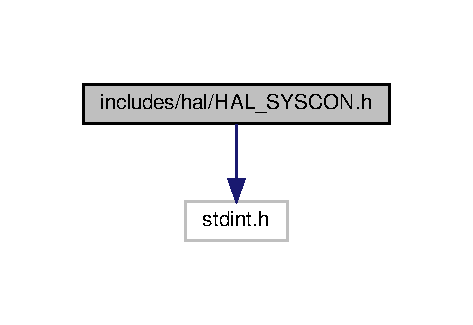
\includegraphics[width=227pt]{HAL__SYSCON_8h__incl}
\end{center}
\end{figure}
Gráfico de los archivos que directa o indirectamente incluyen a este archivo\+:\nopagebreak
\begin{figure}[H]
\begin{center}
\leavevmode
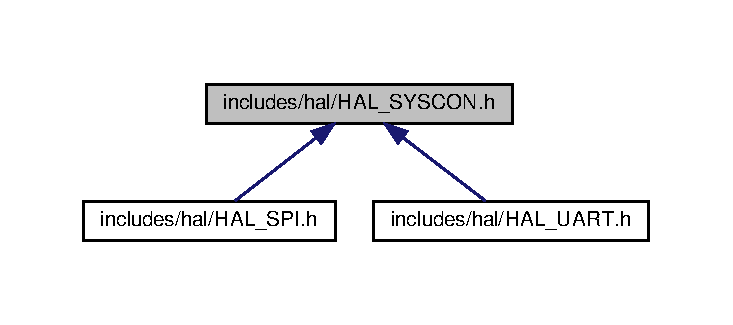
\includegraphics[width=350pt]{HAL__SYSCON_8h__dep__incl}
\end{center}
\end{figure}
\subsection*{Enumeraciones}
\begin{DoxyCompactItemize}
\item 
\mbox{\Hypertarget{HAL__SYSCON_8h_aa23b6654979f5c5d0c6caec99cc336b4}\label{HAL__SYSCON_8h_aa23b6654979f5c5d0c6caec99cc336b4}} 
enum {\bfseries hal\+\_\+syscon\+\_\+clkout\+\_\+source\+\_\+sel\+\_\+en} \{ \newline
{\bfseries H\+A\+L\+\_\+\+S\+Y\+S\+C\+O\+N\+\_\+\+C\+L\+K\+O\+U\+T\+\_\+\+S\+O\+U\+R\+C\+E\+\_\+\+S\+E\+L\+\_\+\+F\+RO} = 0, 
{\bfseries H\+A\+L\+\_\+\+S\+Y\+S\+C\+O\+N\+\_\+\+C\+L\+K\+O\+U\+T\+\_\+\+S\+O\+U\+R\+C\+E\+\_\+\+S\+E\+L\+\_\+\+M\+A\+I\+N\+\_\+\+C\+L\+O\+CK}, 
{\bfseries H\+A\+L\+\_\+\+S\+Y\+S\+C\+O\+N\+\_\+\+C\+L\+K\+O\+U\+T\+\_\+\+S\+O\+U\+R\+C\+E\+\_\+\+S\+E\+L\+\_\+\+S\+Y\+S\+\_\+\+P\+LL}, 
{\bfseries H\+A\+L\+\_\+\+S\+Y\+S\+C\+O\+N\+\_\+\+C\+L\+K\+O\+U\+T\+\_\+\+S\+O\+U\+R\+C\+E\+\_\+\+S\+E\+L\+\_\+\+E\+X\+T\+\_\+\+C\+L\+O\+CK}, 
\newline
{\bfseries H\+A\+L\+\_\+\+S\+Y\+S\+C\+O\+N\+\_\+\+C\+L\+K\+O\+U\+T\+\_\+\+S\+O\+U\+R\+C\+E\+\_\+\+S\+E\+L\+\_\+\+W\+A\+T\+C\+H\+D\+O\+G\+\_\+\+O\+SC}
 \}
\item 
\mbox{\Hypertarget{HAL__SYSCON_8h_ac3c6c02a963d446ae8e9b7c0a71ccdcb}\label{HAL__SYSCON_8h_ac3c6c02a963d446ae8e9b7c0a71ccdcb}} 
enum {\bfseries hal\+\_\+syscon\+\_\+frg\+\_\+clock\+\_\+sel\+\_\+en} \{ {\bfseries H\+A\+L\+\_\+\+S\+Y\+S\+C\+O\+N\+\_\+\+F\+R\+G\+\_\+\+C\+L\+O\+C\+K\+\_\+\+S\+E\+L\+\_\+\+F\+RO} = 0, 
{\bfseries H\+A\+L\+\_\+\+S\+Y\+S\+C\+O\+N\+\_\+\+F\+R\+G\+\_\+\+C\+L\+O\+C\+K\+\_\+\+S\+E\+L\+\_\+\+M\+A\+I\+N\+\_\+\+C\+L\+O\+CK}, 
{\bfseries H\+A\+L\+\_\+\+S\+Y\+S\+C\+O\+N\+\_\+\+F\+R\+G\+\_\+\+C\+L\+O\+C\+K\+\_\+\+S\+E\+L\+\_\+\+S\+Y\+S\+\_\+\+P\+LL}, 
{\bfseries H\+A\+L\+\_\+\+S\+Y\+S\+C\+O\+N\+\_\+\+F\+R\+G\+\_\+\+C\+L\+O\+C\+K\+\_\+\+S\+E\+L\+\_\+\+N\+O\+NE}
 \}
\item 
\mbox{\Hypertarget{HAL__SYSCON_8h_a8f85b75727e34f8c9f8d3c46b44a0ae0}\label{HAL__SYSCON_8h_a8f85b75727e34f8c9f8d3c46b44a0ae0}} 
enum {\bfseries hal\+\_\+syscon\+\_\+peripheral\+\_\+sel\+\_\+en} \{ \newline
{\bfseries H\+A\+L\+\_\+\+S\+Y\+S\+C\+O\+N\+\_\+\+P\+E\+R\+I\+P\+H\+E\+R\+A\+L\+\_\+\+S\+E\+L\+\_\+\+U\+A\+R\+T0} = 0, 
{\bfseries H\+A\+L\+\_\+\+S\+Y\+S\+C\+O\+N\+\_\+\+P\+E\+R\+I\+P\+H\+E\+R\+A\+L\+\_\+\+S\+E\+L\+\_\+\+U\+A\+R\+T1}, 
{\bfseries H\+A\+L\+\_\+\+S\+Y\+S\+C\+O\+N\+\_\+\+P\+E\+R\+I\+P\+H\+E\+R\+A\+L\+\_\+\+S\+E\+L\+\_\+\+U\+A\+R\+T2}, 
{\bfseries H\+A\+L\+\_\+\+S\+Y\+S\+C\+O\+N\+\_\+\+P\+E\+R\+I\+P\+H\+E\+R\+A\+L\+\_\+\+S\+E\+L\+\_\+\+U\+A\+R\+T3}, 
\newline
{\bfseries H\+A\+L\+\_\+\+S\+Y\+S\+C\+O\+N\+\_\+\+P\+E\+R\+I\+P\+H\+E\+R\+A\+L\+\_\+\+S\+E\+L\+\_\+\+U\+A\+R\+T4}, 
{\bfseries H\+A\+L\+\_\+\+S\+Y\+S\+C\+O\+N\+\_\+\+P\+E\+R\+I\+P\+H\+E\+R\+A\+L\+\_\+\+S\+E\+L\+\_\+\+I\+I\+C0}, 
{\bfseries H\+A\+L\+\_\+\+S\+Y\+S\+C\+O\+N\+\_\+\+P\+E\+R\+I\+P\+H\+E\+R\+A\+L\+\_\+\+S\+E\+L\+\_\+\+I\+I\+C1}, 
{\bfseries H\+A\+L\+\_\+\+S\+Y\+S\+C\+O\+N\+\_\+\+P\+E\+R\+I\+P\+H\+E\+R\+A\+L\+\_\+\+S\+E\+L\+\_\+\+I\+I\+C2}, 
\newline
{\bfseries H\+A\+L\+\_\+\+S\+Y\+S\+C\+O\+N\+\_\+\+P\+E\+R\+I\+P\+H\+E\+R\+A\+L\+\_\+\+S\+E\+L\+\_\+\+I\+I\+C3}, 
{\bfseries H\+A\+L\+\_\+\+S\+Y\+S\+C\+O\+N\+\_\+\+P\+E\+R\+I\+P\+H\+E\+R\+A\+L\+\_\+\+S\+E\+L\+\_\+\+S\+P\+I0}, 
{\bfseries H\+A\+L\+\_\+\+S\+Y\+S\+C\+O\+N\+\_\+\+P\+E\+R\+I\+P\+H\+E\+R\+A\+L\+\_\+\+S\+E\+L\+\_\+\+S\+P\+I1}
 \}
\item 
\mbox{\Hypertarget{HAL__SYSCON_8h_a8d1873ed52eb0449a0c12acadcecd47b}\label{HAL__SYSCON_8h_a8d1873ed52eb0449a0c12acadcecd47b}} 
enum {\bfseries hal\+\_\+syscon\+\_\+peripheral\+\_\+clock\+\_\+sel\+\_\+en} \{ \newline
{\bfseries H\+A\+L\+\_\+\+S\+Y\+S\+C\+O\+N\+\_\+\+P\+E\+R\+I\+P\+H\+E\+R\+A\+L\+\_\+\+C\+L\+O\+C\+K\+\_\+\+S\+E\+L\+\_\+\+F\+RO} = 0, 
{\bfseries H\+A\+L\+\_\+\+S\+Y\+S\+C\+O\+N\+\_\+\+P\+E\+R\+I\+P\+H\+E\+R\+A\+L\+\_\+\+C\+L\+O\+C\+K\+\_\+\+S\+E\+L\+\_\+\+M\+A\+IN}, 
{\bfseries H\+A\+L\+\_\+\+S\+Y\+S\+C\+O\+N\+\_\+\+P\+E\+R\+I\+P\+H\+E\+R\+A\+L\+\_\+\+C\+L\+O\+C\+K\+\_\+\+S\+E\+L\+\_\+\+F\+R\+G0}, 
{\bfseries H\+A\+L\+\_\+\+S\+Y\+S\+C\+O\+N\+\_\+\+P\+E\+R\+I\+P\+H\+E\+R\+A\+L\+\_\+\+C\+L\+O\+C\+K\+\_\+\+S\+E\+L\+\_\+\+F\+R\+G1}, 
\newline
{\bfseries H\+A\+L\+\_\+\+S\+Y\+S\+C\+O\+N\+\_\+\+P\+E\+R\+I\+P\+H\+E\+R\+A\+L\+\_\+\+C\+L\+O\+C\+K\+\_\+\+S\+E\+L\+\_\+\+F\+R\+O\+\_\+\+D\+IV}, 
{\bfseries H\+A\+L\+\_\+\+S\+Y\+S\+C\+O\+N\+\_\+\+P\+E\+R\+I\+P\+H\+E\+R\+A\+L\+\_\+\+C\+L\+O\+C\+K\+\_\+\+S\+E\+L\+\_\+\+N\+O\+NE} = 7
 \}
\item 
\mbox{\Hypertarget{HAL__SYSCON_8h_ae6e947aa2e205fb9998ee49ed34314d4}\label{HAL__SYSCON_8h_ae6e947aa2e205fb9998ee49ed34314d4}} 
enum {\bfseries hal\+\_\+syscon\+\_\+iocon\+\_\+glitch\+\_\+sel\+\_\+en} \{ \newline
{\bfseries H\+A\+L\+\_\+\+S\+Y\+S\+C\+O\+N\+\_\+\+I\+O\+C\+O\+N\+\_\+\+G\+L\+I\+T\+C\+H\+\_\+\+S\+E\+L\+\_\+0} = 0, 
{\bfseries H\+A\+L\+\_\+\+S\+Y\+S\+C\+O\+N\+\_\+\+I\+O\+C\+O\+N\+\_\+\+G\+L\+I\+T\+C\+H\+\_\+\+S\+E\+L\+\_\+1}, 
{\bfseries H\+A\+L\+\_\+\+S\+Y\+S\+C\+O\+N\+\_\+\+I\+O\+C\+O\+N\+\_\+\+G\+L\+I\+T\+C\+H\+\_\+\+S\+E\+L\+\_\+2}, 
{\bfseries H\+A\+L\+\_\+\+S\+Y\+S\+C\+O\+N\+\_\+\+I\+O\+C\+O\+N\+\_\+\+G\+L\+I\+T\+C\+H\+\_\+\+S\+E\+L\+\_\+3}, 
\newline
{\bfseries H\+A\+L\+\_\+\+S\+Y\+S\+C\+O\+N\+\_\+\+I\+O\+C\+O\+N\+\_\+\+G\+L\+I\+T\+C\+H\+\_\+\+S\+E\+L\+\_\+4}, 
{\bfseries H\+A\+L\+\_\+\+S\+Y\+S\+C\+O\+N\+\_\+\+I\+O\+C\+O\+N\+\_\+\+G\+L\+I\+T\+C\+H\+\_\+\+S\+E\+L\+\_\+5}, 
{\bfseries H\+A\+L\+\_\+\+S\+Y\+S\+C\+O\+N\+\_\+\+I\+O\+C\+O\+N\+\_\+\+G\+L\+I\+T\+C\+H\+\_\+\+S\+E\+L\+\_\+6}, 
{\bfseries H\+A\+L\+\_\+\+S\+Y\+S\+C\+O\+N\+\_\+\+I\+O\+C\+O\+N\+\_\+\+G\+L\+I\+T\+C\+H\+\_\+\+S\+E\+L\+\_\+7}
 \}
\item 
\mbox{\Hypertarget{HAL__SYSCON_8h_af54a8bad7d8d25e0778c0f74ff90a9b2}\label{HAL__SYSCON_8h_af54a8bad7d8d25e0778c0f74ff90a9b2}} 
enum {\bfseries hal\+\_\+syscon\+\_\+pll\+\_\+source\+\_\+sel\+\_\+en} \{ {\bfseries H\+A\+L\+\_\+\+S\+Y\+S\+C\+O\+N\+\_\+\+P\+L\+L\+\_\+\+S\+O\+U\+R\+C\+E\+\_\+\+S\+E\+L\+\_\+\+F\+RO} = 0, 
{\bfseries H\+A\+L\+\_\+\+S\+Y\+S\+C\+O\+N\+\_\+\+P\+L\+L\+\_\+\+S\+O\+U\+R\+C\+E\+\_\+\+S\+E\+L\+\_\+\+E\+X\+T\+\_\+\+C\+LK}, 
{\bfseries H\+A\+L\+\_\+\+S\+Y\+S\+C\+O\+N\+\_\+\+P\+L\+L\+\_\+\+S\+O\+U\+R\+C\+E\+\_\+\+S\+E\+L\+\_\+\+W\+A\+T\+C\+H\+D\+OG}, 
{\bfseries H\+A\+L\+\_\+\+S\+Y\+S\+C\+O\+N\+\_\+\+P\+L\+L\+\_\+\+S\+O\+U\+R\+C\+E\+\_\+\+S\+E\+L\+\_\+\+F\+R\+O\+\_\+\+D\+IV}
 \}
\end{DoxyCompactItemize}
\subsection*{Funciones}
\begin{DoxyCompactItemize}
\item 
uint32\+\_\+t \hyperlink{HAL__SYSCON_8h_a31c48c74f760fbad8518a0a6c89731eb}{hal\+\_\+syscon\+\_\+get\+\_\+system\+\_\+clock} (void)
\begin{DoxyCompactList}\small\item\em Obtener la frecuencia actual del main clock. \end{DoxyCompactList}\item 
uint32\+\_\+t \hyperlink{HAL__SYSCON_8h_a7768b17907648deb424cb4254ad35d10}{hal\+\_\+syscon\+\_\+get\+\_\+fro\+\_\+clock} (void)
\begin{DoxyCompactList}\small\item\em Obtener la frecuencia actual del F\+RO. \end{DoxyCompactList}\item 
void \hyperlink{HAL__SYSCON_8h_accafad7cb2378e99a09afd26de8d432e}{hal\+\_\+syscon\+\_\+config\+\_\+external\+\_\+crystal} (uint32\+\_\+t crystal\+\_\+freq, uint8\+\_\+t use\+\_\+as\+\_\+main)
\begin{DoxyCompactList}\small\item\em Configurar el ext clock a partir de un cristal externo. \end{DoxyCompactList}\item 
void \hyperlink{HAL__SYSCON_8h_ab6b37d2df55c51dbb27c2c02bb087587}{hal\+\_\+syscon\+\_\+config\+\_\+fro\+\_\+direct} (uint8\+\_\+t direct, uint8\+\_\+t use\+\_\+as\+\_\+main)
\begin{DoxyCompactList}\small\item\em Configurar el clock F\+RO. \end{DoxyCompactList}\item 
void \hyperlink{HAL__SYSCON_8h_a1c2a74ef250399dba55e1f17b43abe38}{hal\+\_\+syscon\+\_\+config\+\_\+clkout} (uint8\+\_\+t port, uint8\+\_\+t pin, hal\+\_\+syscon\+\_\+clkout\+\_\+source\+\_\+sel\+\_\+en clock\+\_\+source, uint8\+\_\+t divider)
\begin{DoxyCompactList}\small\item\em Configurar el pin de clock out (salida de clock hacia afuera) \end{DoxyCompactList}\item 
void \hyperlink{HAL__SYSCON_8h_a5cd176b5be324489a45a8626ec89ce99}{hal\+\_\+syscon\+\_\+config\+\_\+frg} (uint8\+\_\+t inst, hal\+\_\+syscon\+\_\+frg\+\_\+clock\+\_\+sel\+\_\+en clock\+\_\+source, uint32\+\_\+t mul)
\begin{DoxyCompactList}\small\item\em Configurar el divisor fraccional. \end{DoxyCompactList}\item 
void \hyperlink{HAL__SYSCON_8h_aeec2e4ffb8eca74db67bd0ce4c7a06c6}{hal\+\_\+syscon\+\_\+set\+\_\+peripheral\+\_\+clock\+\_\+source} (hal\+\_\+syscon\+\_\+peripheral\+\_\+sel\+\_\+en peripheral, hal\+\_\+syscon\+\_\+peripheral\+\_\+clock\+\_\+sel\+\_\+en clock\+\_\+source)
\begin{DoxyCompactList}\small\item\em Fijar la fuente de clock de un periferico. \end{DoxyCompactList}\item 
uint32\+\_\+t \hyperlink{HAL__SYSCON_8h_ac37805288fe2b5489e7f1d1c5765e298}{hal\+\_\+syscon\+\_\+get\+\_\+peripheral\+\_\+clock} (hal\+\_\+syscon\+\_\+peripheral\+\_\+sel\+\_\+en peripheral)
\begin{DoxyCompactList}\small\item\em Obtener la frecuencia de clock en Hz configurada para cierto periferico. \end{DoxyCompactList}\item 
void \hyperlink{HAL__SYSCON_8h_ac2eb2b4b2c904d02fac721092422edeb}{hal\+\_\+syscon\+\_\+set\+\_\+iocon\+\_\+glitch\+\_\+divider} (hal\+\_\+syscon\+\_\+iocon\+\_\+glitch\+\_\+sel\+\_\+en sel, uint32\+\_\+t div)
\begin{DoxyCompactList}\small\item\em Configurar divisor para el clock de glitches del I\+O\+C\+ON. \end{DoxyCompactList}\item 
void \hyperlink{HAL__SYSCON_8h_aa29b349b8b958efeed0831ed31eadf94}{hal\+\_\+syscon\+\_\+config\+\_\+pll} (hal\+\_\+syscon\+\_\+pll\+\_\+source\+\_\+sel\+\_\+en clock\+\_\+source, uint32\+\_\+t freq)
\begin{DoxyCompactList}\small\item\em Configurar el P\+LL. \end{DoxyCompactList}\item 
uint32\+\_\+t \hyperlink{HAL__SYSCON_8h_aadbb4d022ecc8916c0346b8f537e19d0}{hal\+\_\+syscon\+\_\+get\+\_\+pll\+\_\+clock} (void)
\begin{DoxyCompactList}\small\item\em Obtener frecuencia actual configurada del P\+LL. \end{DoxyCompactList}\end{DoxyCompactItemize}


\subsection{Descripción detallada}
Declaraciones a nivel de aplicacion del periferico S\+Y\+S\+C\+ON (L\+P\+C845) 

\begin{DoxyAuthor}{Autor}
Augusto Santini 
\end{DoxyAuthor}
\begin{DoxyDate}{Fecha}
6/2019 
\end{DoxyDate}
\begin{DoxyVersion}{Versión}
1.\+0 
\end{DoxyVersion}


\subsection{Documentación de las funciones}
\mbox{\Hypertarget{HAL__SYSCON_8h_a31c48c74f760fbad8518a0a6c89731eb}\label{HAL__SYSCON_8h_a31c48c74f760fbad8518a0a6c89731eb}} 
\index{H\+A\+L\+\_\+\+S\+Y\+S\+C\+O\+N.\+h@{H\+A\+L\+\_\+\+S\+Y\+S\+C\+O\+N.\+h}!hal\+\_\+syscon\+\_\+get\+\_\+system\+\_\+clock@{hal\+\_\+syscon\+\_\+get\+\_\+system\+\_\+clock}}
\index{hal\+\_\+syscon\+\_\+get\+\_\+system\+\_\+clock@{hal\+\_\+syscon\+\_\+get\+\_\+system\+\_\+clock}!H\+A\+L\+\_\+\+S\+Y\+S\+C\+O\+N.\+h@{H\+A\+L\+\_\+\+S\+Y\+S\+C\+O\+N.\+h}}
\subsubsection{\texorpdfstring{hal\+\_\+syscon\+\_\+get\+\_\+system\+\_\+clock()}{hal\_syscon\_get\_system\_clock()}}
{\footnotesize\ttfamily uint32\+\_\+t hal\+\_\+syscon\+\_\+get\+\_\+system\+\_\+clock (\begin{DoxyParamCaption}\item[{void}]{ }\end{DoxyParamCaption})}



Obtener la frecuencia actual del main clock. 

\begin{DoxyReturn}{Devuelve}
Frecuencia del main clock en Hz 
\end{DoxyReturn}
\mbox{\Hypertarget{HAL__SYSCON_8h_a7768b17907648deb424cb4254ad35d10}\label{HAL__SYSCON_8h_a7768b17907648deb424cb4254ad35d10}} 
\index{H\+A\+L\+\_\+\+S\+Y\+S\+C\+O\+N.\+h@{H\+A\+L\+\_\+\+S\+Y\+S\+C\+O\+N.\+h}!hal\+\_\+syscon\+\_\+get\+\_\+fro\+\_\+clock@{hal\+\_\+syscon\+\_\+get\+\_\+fro\+\_\+clock}}
\index{hal\+\_\+syscon\+\_\+get\+\_\+fro\+\_\+clock@{hal\+\_\+syscon\+\_\+get\+\_\+fro\+\_\+clock}!H\+A\+L\+\_\+\+S\+Y\+S\+C\+O\+N.\+h@{H\+A\+L\+\_\+\+S\+Y\+S\+C\+O\+N.\+h}}
\subsubsection{\texorpdfstring{hal\+\_\+syscon\+\_\+get\+\_\+fro\+\_\+clock()}{hal\_syscon\_get\_fro\_clock()}}
{\footnotesize\ttfamily uint32\+\_\+t hal\+\_\+syscon\+\_\+get\+\_\+fro\+\_\+clock (\begin{DoxyParamCaption}\item[{void}]{ }\end{DoxyParamCaption})}



Obtener la frecuencia actual del F\+RO. 

\begin{DoxyReturn}{Devuelve}
Frecuencia del F\+RO en Hz 
\end{DoxyReturn}
\mbox{\Hypertarget{HAL__SYSCON_8h_accafad7cb2378e99a09afd26de8d432e}\label{HAL__SYSCON_8h_accafad7cb2378e99a09afd26de8d432e}} 
\index{H\+A\+L\+\_\+\+S\+Y\+S\+C\+O\+N.\+h@{H\+A\+L\+\_\+\+S\+Y\+S\+C\+O\+N.\+h}!hal\+\_\+syscon\+\_\+config\+\_\+external\+\_\+crystal@{hal\+\_\+syscon\+\_\+config\+\_\+external\+\_\+crystal}}
\index{hal\+\_\+syscon\+\_\+config\+\_\+external\+\_\+crystal@{hal\+\_\+syscon\+\_\+config\+\_\+external\+\_\+crystal}!H\+A\+L\+\_\+\+S\+Y\+S\+C\+O\+N.\+h@{H\+A\+L\+\_\+\+S\+Y\+S\+C\+O\+N.\+h}}
\subsubsection{\texorpdfstring{hal\+\_\+syscon\+\_\+config\+\_\+external\+\_\+crystal()}{hal\_syscon\_config\_external\_crystal()}}
{\footnotesize\ttfamily void hal\+\_\+syscon\+\_\+config\+\_\+external\+\_\+crystal (\begin{DoxyParamCaption}\item[{uint32\+\_\+t}]{crystal\+\_\+freq,  }\item[{uint8\+\_\+t}]{use\+\_\+as\+\_\+main }\end{DoxyParamCaption})}



Configurar el ext clock a partir de un cristal externo. 


\begin{DoxyParams}[1]{Parámetros}
\mbox{\tt in}  & {\em crystal\+\_\+freq} & Frecuencia del cristal externo utilizado \\
\hline
\mbox{\tt in}  & {\em use\+\_\+as\+\_\+main} & Si es distinto de cero, se utilizara el oscilador a cristal como main clock \\
\hline
\end{DoxyParams}
\mbox{\Hypertarget{HAL__SYSCON_8h_ab6b37d2df55c51dbb27c2c02bb087587}\label{HAL__SYSCON_8h_ab6b37d2df55c51dbb27c2c02bb087587}} 
\index{H\+A\+L\+\_\+\+S\+Y\+S\+C\+O\+N.\+h@{H\+A\+L\+\_\+\+S\+Y\+S\+C\+O\+N.\+h}!hal\+\_\+syscon\+\_\+config\+\_\+fro\+\_\+direct@{hal\+\_\+syscon\+\_\+config\+\_\+fro\+\_\+direct}}
\index{hal\+\_\+syscon\+\_\+config\+\_\+fro\+\_\+direct@{hal\+\_\+syscon\+\_\+config\+\_\+fro\+\_\+direct}!H\+A\+L\+\_\+\+S\+Y\+S\+C\+O\+N.\+h@{H\+A\+L\+\_\+\+S\+Y\+S\+C\+O\+N.\+h}}
\subsubsection{\texorpdfstring{hal\+\_\+syscon\+\_\+config\+\_\+fro\+\_\+direct()}{hal\_syscon\_config\_fro\_direct()}}
{\footnotesize\ttfamily void hal\+\_\+syscon\+\_\+config\+\_\+fro\+\_\+direct (\begin{DoxyParamCaption}\item[{uint8\+\_\+t}]{direct,  }\item[{uint8\+\_\+t}]{use\+\_\+as\+\_\+main }\end{DoxyParamCaption})}



Configurar el clock F\+RO. 


\begin{DoxyParams}[1]{Parámetros}
\mbox{\tt in}  & {\em direct} & Si es distinto de cero se omite el divisor del F\+RO \\
\hline
\mbox{\tt in}  & {\em use\+\_\+as\+\_\+main} & Si es distinto de cero, se utilizara el F\+RO como main clock \\
\hline
\end{DoxyParams}
\mbox{\Hypertarget{HAL__SYSCON_8h_a1c2a74ef250399dba55e1f17b43abe38}\label{HAL__SYSCON_8h_a1c2a74ef250399dba55e1f17b43abe38}} 
\index{H\+A\+L\+\_\+\+S\+Y\+S\+C\+O\+N.\+h@{H\+A\+L\+\_\+\+S\+Y\+S\+C\+O\+N.\+h}!hal\+\_\+syscon\+\_\+config\+\_\+clkout@{hal\+\_\+syscon\+\_\+config\+\_\+clkout}}
\index{hal\+\_\+syscon\+\_\+config\+\_\+clkout@{hal\+\_\+syscon\+\_\+config\+\_\+clkout}!H\+A\+L\+\_\+\+S\+Y\+S\+C\+O\+N.\+h@{H\+A\+L\+\_\+\+S\+Y\+S\+C\+O\+N.\+h}}
\subsubsection{\texorpdfstring{hal\+\_\+syscon\+\_\+config\+\_\+clkout()}{hal\_syscon\_config\_clkout()}}
{\footnotesize\ttfamily void hal\+\_\+syscon\+\_\+config\+\_\+clkout (\begin{DoxyParamCaption}\item[{uint8\+\_\+t}]{port,  }\item[{uint8\+\_\+t}]{pin,  }\item[{hal\+\_\+syscon\+\_\+clkout\+\_\+source\+\_\+sel\+\_\+en}]{clock\+\_\+source,  }\item[{uint8\+\_\+t}]{divider }\end{DoxyParamCaption})}



Configurar el pin de clock out (salida de clock hacia afuera) 


\begin{DoxyParams}[1]{Parámetros}
\mbox{\tt in}  & {\em port} & Numero de puerto por donde sacar el clock out \\
\hline
\mbox{\tt in}  & {\em pin} & Numero de pin por donde sacar el clock out \\
\hline
\mbox{\tt in}  & {\em clock\+\_\+source} & Fuente deseada para la salida clock out \\
\hline
\mbox{\tt in}  & {\em divider} & Divisor deseado para la salida clock out \\
\hline
\end{DoxyParams}
\mbox{\Hypertarget{HAL__SYSCON_8h_a5cd176b5be324489a45a8626ec89ce99}\label{HAL__SYSCON_8h_a5cd176b5be324489a45a8626ec89ce99}} 
\index{H\+A\+L\+\_\+\+S\+Y\+S\+C\+O\+N.\+h@{H\+A\+L\+\_\+\+S\+Y\+S\+C\+O\+N.\+h}!hal\+\_\+syscon\+\_\+config\+\_\+frg@{hal\+\_\+syscon\+\_\+config\+\_\+frg}}
\index{hal\+\_\+syscon\+\_\+config\+\_\+frg@{hal\+\_\+syscon\+\_\+config\+\_\+frg}!H\+A\+L\+\_\+\+S\+Y\+S\+C\+O\+N.\+h@{H\+A\+L\+\_\+\+S\+Y\+S\+C\+O\+N.\+h}}
\subsubsection{\texorpdfstring{hal\+\_\+syscon\+\_\+config\+\_\+frg()}{hal\_syscon\_config\_frg()}}
{\footnotesize\ttfamily void hal\+\_\+syscon\+\_\+config\+\_\+frg (\begin{DoxyParamCaption}\item[{uint8\+\_\+t}]{inst,  }\item[{hal\+\_\+syscon\+\_\+frg\+\_\+clock\+\_\+sel\+\_\+en}]{clock\+\_\+source,  }\item[{uint32\+\_\+t}]{mul }\end{DoxyParamCaption})}



Configurar el divisor fraccional. 

El divisor siempre se debe fijar en 256 para estos M\+CU.


\begin{DoxyParams}[1]{Parámetros}
\mbox{\tt in}  & {\em inst} & Instancia de F\+RG a configurar \\
\hline
\mbox{\tt in}  & {\em clock\+\_\+source} & Fuente de clock de entrada para el F\+RG \\
\hline
\mbox{\tt in}  & {\em mul} & Multiplicador deseado \\
\hline
\end{DoxyParams}
\mbox{\Hypertarget{HAL__SYSCON_8h_aeec2e4ffb8eca74db67bd0ce4c7a06c6}\label{HAL__SYSCON_8h_aeec2e4ffb8eca74db67bd0ce4c7a06c6}} 
\index{H\+A\+L\+\_\+\+S\+Y\+S\+C\+O\+N.\+h@{H\+A\+L\+\_\+\+S\+Y\+S\+C\+O\+N.\+h}!hal\+\_\+syscon\+\_\+set\+\_\+peripheral\+\_\+clock\+\_\+source@{hal\+\_\+syscon\+\_\+set\+\_\+peripheral\+\_\+clock\+\_\+source}}
\index{hal\+\_\+syscon\+\_\+set\+\_\+peripheral\+\_\+clock\+\_\+source@{hal\+\_\+syscon\+\_\+set\+\_\+peripheral\+\_\+clock\+\_\+source}!H\+A\+L\+\_\+\+S\+Y\+S\+C\+O\+N.\+h@{H\+A\+L\+\_\+\+S\+Y\+S\+C\+O\+N.\+h}}
\subsubsection{\texorpdfstring{hal\+\_\+syscon\+\_\+set\+\_\+peripheral\+\_\+clock\+\_\+source()}{hal\_syscon\_set\_peripheral\_clock\_source()}}
{\footnotesize\ttfamily void hal\+\_\+syscon\+\_\+set\+\_\+peripheral\+\_\+clock\+\_\+source (\begin{DoxyParamCaption}\item[{hal\+\_\+syscon\+\_\+peripheral\+\_\+sel\+\_\+en}]{peripheral,  }\item[{hal\+\_\+syscon\+\_\+peripheral\+\_\+clock\+\_\+sel\+\_\+en}]{clock\+\_\+source }\end{DoxyParamCaption})}



Fijar la fuente de clock de un periferico. 


\begin{DoxyParams}[1]{Parámetros}
\mbox{\tt in}  & {\em peripheral} & Periferico deseado \\
\hline
\mbox{\tt in}  & {\em clock\+\_\+source} & Fuente de clock deseada \\
\hline
\end{DoxyParams}
\mbox{\Hypertarget{HAL__SYSCON_8h_ac37805288fe2b5489e7f1d1c5765e298}\label{HAL__SYSCON_8h_ac37805288fe2b5489e7f1d1c5765e298}} 
\index{H\+A\+L\+\_\+\+S\+Y\+S\+C\+O\+N.\+h@{H\+A\+L\+\_\+\+S\+Y\+S\+C\+O\+N.\+h}!hal\+\_\+syscon\+\_\+get\+\_\+peripheral\+\_\+clock@{hal\+\_\+syscon\+\_\+get\+\_\+peripheral\+\_\+clock}}
\index{hal\+\_\+syscon\+\_\+get\+\_\+peripheral\+\_\+clock@{hal\+\_\+syscon\+\_\+get\+\_\+peripheral\+\_\+clock}!H\+A\+L\+\_\+\+S\+Y\+S\+C\+O\+N.\+h@{H\+A\+L\+\_\+\+S\+Y\+S\+C\+O\+N.\+h}}
\subsubsection{\texorpdfstring{hal\+\_\+syscon\+\_\+get\+\_\+peripheral\+\_\+clock()}{hal\_syscon\_get\_peripheral\_clock()}}
{\footnotesize\ttfamily uint32\+\_\+t hal\+\_\+syscon\+\_\+get\+\_\+peripheral\+\_\+clock (\begin{DoxyParamCaption}\item[{hal\+\_\+syscon\+\_\+peripheral\+\_\+sel\+\_\+en}]{peripheral }\end{DoxyParamCaption})}



Obtener la frecuencia de clock en Hz configurada para cierto periferico. 


\begin{DoxyParams}[1]{Parámetros}
\mbox{\tt in}  & {\em peripheral} & Periferico deseado \\
\hline
\end{DoxyParams}
\begin{DoxyReturn}{Devuelve}
Frecuencia en Hz del clock del periferico 
\end{DoxyReturn}
\mbox{\Hypertarget{HAL__SYSCON_8h_ac2eb2b4b2c904d02fac721092422edeb}\label{HAL__SYSCON_8h_ac2eb2b4b2c904d02fac721092422edeb}} 
\index{H\+A\+L\+\_\+\+S\+Y\+S\+C\+O\+N.\+h@{H\+A\+L\+\_\+\+S\+Y\+S\+C\+O\+N.\+h}!hal\+\_\+syscon\+\_\+set\+\_\+iocon\+\_\+glitch\+\_\+divider@{hal\+\_\+syscon\+\_\+set\+\_\+iocon\+\_\+glitch\+\_\+divider}}
\index{hal\+\_\+syscon\+\_\+set\+\_\+iocon\+\_\+glitch\+\_\+divider@{hal\+\_\+syscon\+\_\+set\+\_\+iocon\+\_\+glitch\+\_\+divider}!H\+A\+L\+\_\+\+S\+Y\+S\+C\+O\+N.\+h@{H\+A\+L\+\_\+\+S\+Y\+S\+C\+O\+N.\+h}}
\subsubsection{\texorpdfstring{hal\+\_\+syscon\+\_\+set\+\_\+iocon\+\_\+glitch\+\_\+divider()}{hal\_syscon\_set\_iocon\_glitch\_divider()}}
{\footnotesize\ttfamily void hal\+\_\+syscon\+\_\+set\+\_\+iocon\+\_\+glitch\+\_\+divider (\begin{DoxyParamCaption}\item[{hal\+\_\+syscon\+\_\+iocon\+\_\+glitch\+\_\+sel\+\_\+en}]{sel,  }\item[{uint32\+\_\+t}]{div }\end{DoxyParamCaption})}



Configurar divisor para el clock de glitches del I\+O\+C\+ON. 


\begin{DoxyParams}[1]{Parámetros}
\mbox{\tt in}  & {\em sel} & Seleccion de divisor \\
\hline
\mbox{\tt in}  & {\em div} & Valor de division deseado \\
\hline
\end{DoxyParams}
\mbox{\Hypertarget{HAL__SYSCON_8h_aa29b349b8b958efeed0831ed31eadf94}\label{HAL__SYSCON_8h_aa29b349b8b958efeed0831ed31eadf94}} 
\index{H\+A\+L\+\_\+\+S\+Y\+S\+C\+O\+N.\+h@{H\+A\+L\+\_\+\+S\+Y\+S\+C\+O\+N.\+h}!hal\+\_\+syscon\+\_\+config\+\_\+pll@{hal\+\_\+syscon\+\_\+config\+\_\+pll}}
\index{hal\+\_\+syscon\+\_\+config\+\_\+pll@{hal\+\_\+syscon\+\_\+config\+\_\+pll}!H\+A\+L\+\_\+\+S\+Y\+S\+C\+O\+N.\+h@{H\+A\+L\+\_\+\+S\+Y\+S\+C\+O\+N.\+h}}
\subsubsection{\texorpdfstring{hal\+\_\+syscon\+\_\+config\+\_\+pll()}{hal\_syscon\_config\_pll()}}
{\footnotesize\ttfamily void hal\+\_\+syscon\+\_\+config\+\_\+pll (\begin{DoxyParamCaption}\item[{hal\+\_\+syscon\+\_\+pll\+\_\+source\+\_\+sel\+\_\+en}]{clock\+\_\+source,  }\item[{uint32\+\_\+t}]{freq }\end{DoxyParamCaption})}



Configurar el P\+LL. 


\begin{DoxyParams}[1]{Parámetros}
\mbox{\tt in}  & {\em clock\+\_\+source} & Fuente de clock de referencia para el P\+LL \\
\hline
\mbox{\tt in}  & {\em freq} & Frecuencia deseada de salida del P\+LL \\
\hline
\end{DoxyParams}
\mbox{\Hypertarget{HAL__SYSCON_8h_aadbb4d022ecc8916c0346b8f537e19d0}\label{HAL__SYSCON_8h_aadbb4d022ecc8916c0346b8f537e19d0}} 
\index{H\+A\+L\+\_\+\+S\+Y\+S\+C\+O\+N.\+h@{H\+A\+L\+\_\+\+S\+Y\+S\+C\+O\+N.\+h}!hal\+\_\+syscon\+\_\+get\+\_\+pll\+\_\+clock@{hal\+\_\+syscon\+\_\+get\+\_\+pll\+\_\+clock}}
\index{hal\+\_\+syscon\+\_\+get\+\_\+pll\+\_\+clock@{hal\+\_\+syscon\+\_\+get\+\_\+pll\+\_\+clock}!H\+A\+L\+\_\+\+S\+Y\+S\+C\+O\+N.\+h@{H\+A\+L\+\_\+\+S\+Y\+S\+C\+O\+N.\+h}}
\subsubsection{\texorpdfstring{hal\+\_\+syscon\+\_\+get\+\_\+pll\+\_\+clock()}{hal\_syscon\_get\_pll\_clock()}}
{\footnotesize\ttfamily uint32\+\_\+t hal\+\_\+syscon\+\_\+get\+\_\+pll\+\_\+clock (\begin{DoxyParamCaption}\item[{void}]{ }\end{DoxyParamCaption})}



Obtener frecuencia actual configurada del P\+LL. 

\begin{DoxyReturn}{Devuelve}
Frecuencia actual del P\+LL en Hz 
\end{DoxyReturn}

\hypertarget{HAL__SYSTICK_8h}{}\section{Referencia del Archivo includes/hal/\+H\+A\+L\+\_\+\+S\+Y\+S\+T\+I\+CK.h}
\label{HAL__SYSTICK_8h}\index{includes/hal/\+H\+A\+L\+\_\+\+S\+Y\+S\+T\+I\+C\+K.\+h@{includes/hal/\+H\+A\+L\+\_\+\+S\+Y\+S\+T\+I\+C\+K.\+h}}


Declaraciones a nivel de aplicacion del periferico S\+Y\+S\+I\+CK (L\+P\+C845)  


{\ttfamily \#include $<$stdint.\+h$>$}\newline
Dependencia gráfica adjunta para H\+A\+L\+\_\+\+S\+Y\+S\+T\+I\+C\+K.\+h\+:
\nopagebreak
\begin{figure}[H]
\begin{center}
\leavevmode
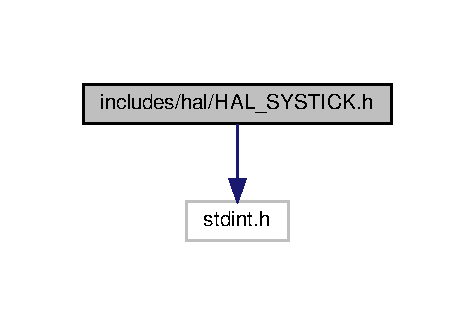
\includegraphics[width=228pt]{HAL__SYSTICK_8h__incl}
\end{center}
\end{figure}
\subsection*{Funciones}
\begin{DoxyCompactItemize}
\item 
void \hyperlink{HAL__SYSTICK_8h_a29eb17e59d26a3f1a1f9184154964f36}{hal\+\_\+systick\+\_\+init} (uint32\+\_\+t tick\+\_\+us, void($\ast$callback)(void))
\begin{DoxyCompactList}\small\item\em Inicializacion del S\+Y\+S\+T\+I\+CK. \end{DoxyCompactList}\item 
void \hyperlink{HAL__SYSTICK_8h_a7291cb0d9994e019d2b2e804f454b571}{hal\+\_\+systick\+\_\+update\+\_\+callback} (void($\ast$callback)(void))
\begin{DoxyCompactList}\small\item\em Actualizar callback del S\+Y\+S\+T\+I\+CK. \end{DoxyCompactList}\end{DoxyCompactItemize}


\subsection{Descripción detallada}
Declaraciones a nivel de aplicacion del periferico S\+Y\+S\+I\+CK (L\+P\+C845) 

\begin{DoxyAuthor}{Autor}
Augusto Santini 
\end{DoxyAuthor}
\begin{DoxyDate}{Fecha}
3/2020 
\end{DoxyDate}
\begin{DoxyVersion}{Versión}
1.\+0 
\end{DoxyVersion}


\subsection{Documentación de las funciones}
\mbox{\Hypertarget{HAL__SYSTICK_8h_a29eb17e59d26a3f1a1f9184154964f36}\label{HAL__SYSTICK_8h_a29eb17e59d26a3f1a1f9184154964f36}} 
\index{H\+A\+L\+\_\+\+S\+Y\+S\+T\+I\+C\+K.\+h@{H\+A\+L\+\_\+\+S\+Y\+S\+T\+I\+C\+K.\+h}!hal\+\_\+systick\+\_\+init@{hal\+\_\+systick\+\_\+init}}
\index{hal\+\_\+systick\+\_\+init@{hal\+\_\+systick\+\_\+init}!H\+A\+L\+\_\+\+S\+Y\+S\+T\+I\+C\+K.\+h@{H\+A\+L\+\_\+\+S\+Y\+S\+T\+I\+C\+K.\+h}}
\subsubsection{\texorpdfstring{hal\+\_\+systick\+\_\+init()}{hal\_systick\_init()}}
{\footnotesize\ttfamily void hal\+\_\+systick\+\_\+init (\begin{DoxyParamCaption}\item[{uint32\+\_\+t}]{tick\+\_\+us,  }\item[{void($\ast$)(void)}]{callback }\end{DoxyParamCaption})}



Inicializacion del S\+Y\+S\+T\+I\+CK. 


\begin{DoxyParams}[1]{Parámetros}
\mbox{\tt in}  & {\em tick\+\_\+us} & Tiempo en microsegundos deseado para el tick \\
\hline
\mbox{\tt in}  & {\em callback} & Funcion a llamar en cada tick \\
\hline
\end{DoxyParams}
\begin{Desc}
\item[Ejemplos\+: ]\par
\hyperlink{Ejemplo_ADC_8c-example}{Ejemplo\+\_\+\+A\+D\+C.\+c}.\end{Desc}
\mbox{\Hypertarget{HAL__SYSTICK_8h_a7291cb0d9994e019d2b2e804f454b571}\label{HAL__SYSTICK_8h_a7291cb0d9994e019d2b2e804f454b571}} 
\index{H\+A\+L\+\_\+\+S\+Y\+S\+T\+I\+C\+K.\+h@{H\+A\+L\+\_\+\+S\+Y\+S\+T\+I\+C\+K.\+h}!hal\+\_\+systick\+\_\+update\+\_\+callback@{hal\+\_\+systick\+\_\+update\+\_\+callback}}
\index{hal\+\_\+systick\+\_\+update\+\_\+callback@{hal\+\_\+systick\+\_\+update\+\_\+callback}!H\+A\+L\+\_\+\+S\+Y\+S\+T\+I\+C\+K.\+h@{H\+A\+L\+\_\+\+S\+Y\+S\+T\+I\+C\+K.\+h}}
\subsubsection{\texorpdfstring{hal\+\_\+systick\+\_\+update\+\_\+callback()}{hal\_systick\_update\_callback()}}
{\footnotesize\ttfamily void hal\+\_\+systick\+\_\+update\+\_\+callback (\begin{DoxyParamCaption}\item[{void($\ast$)(void)}]{callback }\end{DoxyParamCaption})}



Actualizar callback del S\+Y\+S\+T\+I\+CK. 


\begin{DoxyParams}[1]{Parámetros}
\mbox{\tt in}  & {\em callback} & Nuevo callback a ejecutar en cada tick \\
\hline
\end{DoxyParams}

\hypertarget{HAL__UART_8h}{}\doxysection{Referencia del Archivo includes/hal/\+H\+A\+L\+\_\+\+U\+A\+RT.h}
\label{HAL__UART_8h}\index{includes/hal/HAL\_UART.h@{includes/hal/HAL\_UART.h}}


Declaraciones a nivel de aplicacion del periferico U\+A\+RT (L\+P\+C845)  


{\ttfamily \#include $<$stdint.\+h$>$}\newline
{\ttfamily \#include $<$H\+A\+L\+\_\+\+S\+Y\+S\+C\+O\+N.\+h$>$}\newline
{\ttfamily \#include $<$H\+A\+L\+\_\+\+G\+P\+I\+O.\+h$>$}\newline
Dependencia gráfica adjunta para H\+A\+L\+\_\+\+U\+A\+R\+T.\+h\+:\nopagebreak
\begin{figure}[H]
\begin{center}
\leavevmode
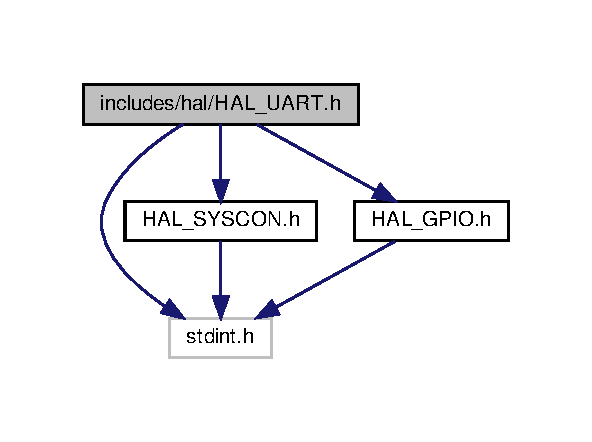
\includegraphics[width=284pt]{HAL__UART_8h__incl}
\end{center}
\end{figure}
\doxysubsection*{Estructuras de datos}
\begin{DoxyCompactItemize}
\item 
struct \mbox{\hyperlink{structhal__uart__config__t}{hal\+\_\+uart\+\_\+config\+\_\+t}}
\end{DoxyCompactItemize}
\doxysubsection*{Enumeraciones}
\begin{DoxyCompactItemize}
\item 
\mbox{\Hypertarget{HAL__UART_8h_a7eb9eb1e60b93c109e14ac618ab7901e}\label{HAL__UART_8h_a7eb9eb1e60b93c109e14ac618ab7901e}} 
enum {\bfseries hal\+\_\+uart\+\_\+datalen\+\_\+en} \{ {\bfseries H\+A\+L\+\_\+\+U\+A\+R\+T\+\_\+\+D\+A\+T\+A\+L\+E\+N\+\_\+7\+B\+IT} = 0, 
{\bfseries H\+A\+L\+\_\+\+U\+A\+R\+T\+\_\+\+D\+A\+T\+A\+L\+E\+N\+\_\+8\+B\+IT}, 
{\bfseries H\+A\+L\+\_\+\+U\+A\+R\+T\+\_\+\+D\+A\+T\+A\+L\+E\+N\+\_\+9\+B\+IT}
 \}
\item 
\mbox{\Hypertarget{HAL__UART_8h_a220ffe3b05d04a08e12a6193549511d1}\label{HAL__UART_8h_a220ffe3b05d04a08e12a6193549511d1}} 
enum {\bfseries hal\+\_\+uart\+\_\+parity\+\_\+en} \{ {\bfseries H\+A\+L\+\_\+\+U\+A\+R\+T\+\_\+\+P\+A\+R\+I\+T\+Y\+\_\+\+N\+O\+\_\+\+P\+A\+R\+I\+TY} = 0, 
{\bfseries H\+A\+L\+\_\+\+U\+A\+R\+T\+\_\+\+P\+A\+R\+I\+T\+Y\+\_\+\+E\+V\+EN} = 2, 
{\bfseries H\+A\+L\+\_\+\+U\+A\+R\+T\+\_\+\+P\+A\+R\+I\+T\+Y\+\_\+\+O\+DD}
 \}
\item 
\mbox{\Hypertarget{HAL__UART_8h_a55a5b3c508317c2fdbc41525d7c8bc97}\label{HAL__UART_8h_a55a5b3c508317c2fdbc41525d7c8bc97}} 
enum {\bfseries hal\+\_\+uart\+\_\+stop\+\_\+en} \{ {\bfseries H\+A\+L\+\_\+\+U\+A\+R\+T\+\_\+\+S\+T\+O\+P\+L\+E\+N\+\_\+1\+B\+IT} = 0, 
{\bfseries H\+A\+L\+\_\+\+U\+A\+R\+T\+\_\+\+S\+T\+O\+P\+L\+E\+N\+\_\+2\+B\+IT}
 \}
\item 
\mbox{\Hypertarget{HAL__UART_8h_a43bd29e1a1f8591ef801d070f55afc93}\label{HAL__UART_8h_a43bd29e1a1f8591ef801d070f55afc93}} 
enum {\bfseries hal\+\_\+uart\+\_\+oversampling\+\_\+en} \{ \newline
{\bfseries H\+A\+L\+\_\+\+U\+A\+R\+T\+\_\+\+O\+V\+E\+R\+S\+A\+M\+P\+L\+I\+N\+G\+\_\+\+X5} = 4, 
{\bfseries H\+A\+L\+\_\+\+U\+A\+R\+T\+\_\+\+O\+V\+E\+R\+S\+A\+M\+P\+L\+I\+N\+G\+\_\+\+X6}, 
{\bfseries H\+A\+L\+\_\+\+U\+A\+R\+T\+\_\+\+O\+V\+E\+R\+S\+A\+M\+P\+L\+I\+N\+G\+\_\+\+X7}, 
{\bfseries H\+A\+L\+\_\+\+U\+A\+R\+T\+\_\+\+O\+V\+E\+R\+S\+A\+M\+P\+L\+I\+N\+G\+\_\+\+X8}, 
\newline
{\bfseries H\+A\+L\+\_\+\+U\+A\+R\+T\+\_\+\+O\+V\+E\+R\+S\+A\+M\+P\+L\+I\+N\+G\+\_\+\+X9}, 
{\bfseries H\+A\+L\+\_\+\+U\+A\+R\+T\+\_\+\+O\+V\+E\+R\+S\+A\+M\+P\+L\+I\+N\+G\+\_\+\+X10}, 
{\bfseries H\+A\+L\+\_\+\+U\+A\+R\+T\+\_\+\+O\+V\+E\+R\+S\+A\+M\+P\+L\+I\+N\+G\+\_\+\+X11}, 
{\bfseries H\+A\+L\+\_\+\+U\+A\+R\+T\+\_\+\+O\+V\+E\+R\+S\+A\+M\+P\+L\+I\+N\+G\+\_\+\+X12}, 
\newline
{\bfseries H\+A\+L\+\_\+\+U\+A\+R\+T\+\_\+\+O\+V\+E\+R\+S\+A\+M\+P\+L\+I\+N\+G\+\_\+\+X13}, 
{\bfseries H\+A\+L\+\_\+\+U\+A\+R\+T\+\_\+\+O\+V\+E\+R\+S\+A\+M\+P\+L\+I\+N\+G\+\_\+\+X14}, 
{\bfseries H\+A\+L\+\_\+\+U\+A\+R\+T\+\_\+\+O\+V\+E\+R\+S\+A\+M\+P\+L\+I\+N\+G\+\_\+\+X15}, 
{\bfseries H\+A\+L\+\_\+\+U\+A\+R\+T\+\_\+\+O\+V\+E\+R\+S\+A\+M\+P\+L\+I\+N\+G\+\_\+\+X16}
 \}
\item 
\mbox{\Hypertarget{HAL__UART_8h_a901ade8c04909ed853a3e232aaecff10}\label{HAL__UART_8h_a901ade8c04909ed853a3e232aaecff10}} 
enum {\bfseries hal\+\_\+uart\+\_\+tx\+\_\+result} \{ {\bfseries H\+A\+L\+\_\+\+U\+A\+R\+T\+\_\+\+T\+X\+\_\+\+R\+E\+S\+U\+L\+T\+\_\+\+OK} = 0, 
{\bfseries H\+A\+L\+\_\+\+U\+A\+R\+T\+\_\+\+T\+X\+\_\+\+R\+E\+S\+U\+L\+T\+\_\+\+N\+O\+T\+\_\+\+R\+E\+A\+DY}
 \}
\item 
\mbox{\Hypertarget{HAL__UART_8h_a165cd0258bebd3dbfaaeb878b3e4a611}\label{HAL__UART_8h_a165cd0258bebd3dbfaaeb878b3e4a611}} 
enum {\bfseries hal\+\_\+uart\+\_\+rx\+\_\+result} \{ {\bfseries H\+A\+L\+\_\+\+U\+A\+R\+T\+\_\+\+R\+X\+\_\+\+R\+E\+S\+U\+L\+T\+\_\+\+OK} = 0, 
{\bfseries H\+A\+L\+\_\+\+U\+A\+R\+T\+\_\+\+R\+X\+\_\+\+R\+E\+S\+U\+L\+T\+\_\+\+N\+O\+T\+\_\+\+R\+E\+A\+DY}
 \}
\end{DoxyCompactItemize}
\doxysubsection*{Funciones}
\begin{DoxyCompactItemize}
\item 
void \mbox{\hyperlink{HAL__UART_8h_ae847e2762fdcf69766487fbea2eed69a}{hal\+\_\+uart\+\_\+init}} (uint8\+\_\+t inst, const \mbox{\hyperlink{structhal__uart__config__t}{hal\+\_\+uart\+\_\+config\+\_\+t}} $\ast$config)
\begin{DoxyCompactList}\small\item\em Inicializar U\+A\+RT con los parametros deseados. \end{DoxyCompactList}\item 
hal\+\_\+uart\+\_\+tx\+\_\+result \mbox{\hyperlink{HAL__UART_8h_aac3ebe57d6954db26baedbafdc64fb26}{hal\+\_\+uart\+\_\+tx\+\_\+byte}} (uint8\+\_\+t inst, uint32\+\_\+t data)
\begin{DoxyCompactList}\small\item\em Transmitir un dato mediante la U\+A\+RT. \end{DoxyCompactList}\item 
hal\+\_\+uart\+\_\+rx\+\_\+result \mbox{\hyperlink{HAL__UART_8h_aa9186f2bbb7ce6c298e4e6249341a99a}{hal\+\_\+uart\+\_\+rx\+\_\+byte}} (uint8\+\_\+t inst, uint32\+\_\+t $\ast$data)
\begin{DoxyCompactList}\small\item\em Recibir un dato de la U\+A\+RT. \end{DoxyCompactList}\item 
void \mbox{\hyperlink{HAL__UART_8h_a014876b7037b10d418c3b2006f894f1e}{hal\+\_\+uart\+\_\+register\+\_\+tx\+\_\+callback}} (uint8\+\_\+t inst, void($\ast$new\+\_\+callback)(void))
\begin{DoxyCompactList}\small\item\em Registrar el callback a ser llamado una vez finalizada la transmision de un dato por U\+A\+RT. \end{DoxyCompactList}\item 
void \mbox{\hyperlink{HAL__UART_8h_a07491f4d61942f763b49526e81e2a35d}{hal\+\_\+uart\+\_\+register\+\_\+rx\+\_\+callback}} (uint8\+\_\+t inst, void($\ast$new\+\_\+callback)(void))
\begin{DoxyCompactList}\small\item\em Registrar el callback a ser llamado en la recepcion de un dato por U\+A\+RT. \end{DoxyCompactList}\item 
\mbox{\Hypertarget{HAL__UART_8h_a7a61d73fd6ad0a670c4225140fefd7bd}\label{HAL__UART_8h_a7a61d73fd6ad0a670c4225140fefd7bd}} 
void \mbox{\hyperlink{HAL__UART_8h_a7a61d73fd6ad0a670c4225140fefd7bd}{U\+A\+R\+T3\+\_\+irq}} (void)
\begin{DoxyCompactList}\small\item\em Interrupcion de U\+A\+R\+T3. \end{DoxyCompactList}\item 
\mbox{\Hypertarget{HAL__UART_8h_a28aab3f4a90a2a9d61d88048637c0811}\label{HAL__UART_8h_a28aab3f4a90a2a9d61d88048637c0811}} 
void \mbox{\hyperlink{HAL__UART_8h_a28aab3f4a90a2a9d61d88048637c0811}{U\+A\+R\+T4\+\_\+irq}} (void)
\begin{DoxyCompactList}\small\item\em Interrupcion de U\+A\+R\+T4. \end{DoxyCompactList}\end{DoxyCompactItemize}


\doxysubsection{Descripción detallada}
Declaraciones a nivel de aplicacion del periferico U\+A\+RT (L\+P\+C845) 

\begin{DoxyAuthor}{Autor}
Augusto Santini 
\end{DoxyAuthor}
\begin{DoxyDate}{Fecha}
3/2020 
\end{DoxyDate}
\begin{DoxyVersion}{Versión}
1.\+0 
\end{DoxyVersion}


\doxysubsection{Documentación de las funciones}
\mbox{\Hypertarget{HAL__UART_8h_ae847e2762fdcf69766487fbea2eed69a}\label{HAL__UART_8h_ae847e2762fdcf69766487fbea2eed69a}} 
\index{HAL\_UART.h@{HAL\_UART.h}!hal\_uart\_init@{hal\_uart\_init}}
\index{hal\_uart\_init@{hal\_uart\_init}!HAL\_UART.h@{HAL\_UART.h}}
\doxysubsubsection{\texorpdfstring{hal\_uart\_init()}{hal\_uart\_init()}}
{\footnotesize\ttfamily void hal\+\_\+uart\+\_\+init (\begin{DoxyParamCaption}\item[{uint8\+\_\+t}]{inst,  }\item[{const \mbox{\hyperlink{structhal__uart__config__t}{hal\+\_\+uart\+\_\+config\+\_\+t}} $\ast$}]{config }\end{DoxyParamCaption})}



Inicializar U\+A\+RT con los parametros deseados. 


\begin{DoxyParams}[1]{Parámetros}
\mbox{\texttt{ in}}  & {\em inst} & Que instancia de U\+A\+RT inicializar \\
\hline
\mbox{\texttt{ in}}  & {\em config} & Puntero a configuracion de la U\+A\+RT \\
\hline
\end{DoxyParams}
\mbox{\Hypertarget{HAL__UART_8h_aac3ebe57d6954db26baedbafdc64fb26}\label{HAL__UART_8h_aac3ebe57d6954db26baedbafdc64fb26}} 
\index{HAL\_UART.h@{HAL\_UART.h}!hal\_uart\_tx\_byte@{hal\_uart\_tx\_byte}}
\index{hal\_uart\_tx\_byte@{hal\_uart\_tx\_byte}!HAL\_UART.h@{HAL\_UART.h}}
\doxysubsubsection{\texorpdfstring{hal\_uart\_tx\_byte()}{hal\_uart\_tx\_byte()}}
{\footnotesize\ttfamily hal\+\_\+uart\+\_\+tx\+\_\+result hal\+\_\+uart\+\_\+tx\+\_\+byte (\begin{DoxyParamCaption}\item[{uint8\+\_\+t}]{inst,  }\item[{uint32\+\_\+t}]{data }\end{DoxyParamCaption})}



Transmitir un dato mediante la U\+A\+RT. 


\begin{DoxyParams}[1]{Parámetros}
\mbox{\texttt{ in}}  & {\em inst} & Que instancia de U\+A\+RT usar \\
\hline
\mbox{\texttt{ in}}  & {\em data} & Dato a transmitir. Puede ser de 7, 8 o 9 bits \\
\hline
\end{DoxyParams}
\mbox{\Hypertarget{HAL__UART_8h_aa9186f2bbb7ce6c298e4e6249341a99a}\label{HAL__UART_8h_aa9186f2bbb7ce6c298e4e6249341a99a}} 
\index{HAL\_UART.h@{HAL\_UART.h}!hal\_uart\_rx\_byte@{hal\_uart\_rx\_byte}}
\index{hal\_uart\_rx\_byte@{hal\_uart\_rx\_byte}!HAL\_UART.h@{HAL\_UART.h}}
\doxysubsubsection{\texorpdfstring{hal\_uart\_rx\_byte()}{hal\_uart\_rx\_byte()}}
{\footnotesize\ttfamily hal\+\_\+uart\+\_\+rx\+\_\+result hal\+\_\+uart\+\_\+rx\+\_\+byte (\begin{DoxyParamCaption}\item[{uint8\+\_\+t}]{inst,  }\item[{uint32\+\_\+t $\ast$}]{data }\end{DoxyParamCaption})}



Recibir un dato de la U\+A\+RT. 


\begin{DoxyParams}[1]{Parámetros}
\mbox{\texttt{ in}}  & {\em inst} & Que instancia de U\+A\+RT usar \\
\hline
\mbox{\texttt{ in}}  & {\em data} & Puntero a donde guardar el dato recibido \\
\hline
\end{DoxyParams}
\begin{DoxyReturn}{Devuelve}
Estado de la recepcion 
\end{DoxyReturn}
\mbox{\Hypertarget{HAL__UART_8h_a014876b7037b10d418c3b2006f894f1e}\label{HAL__UART_8h_a014876b7037b10d418c3b2006f894f1e}} 
\index{HAL\_UART.h@{HAL\_UART.h}!hal\_uart\_register\_tx\_callback@{hal\_uart\_register\_tx\_callback}}
\index{hal\_uart\_register\_tx\_callback@{hal\_uart\_register\_tx\_callback}!HAL\_UART.h@{HAL\_UART.h}}
\doxysubsubsection{\texorpdfstring{hal\_uart\_register\_tx\_callback()}{hal\_uart\_register\_tx\_callback()}}
{\footnotesize\ttfamily void hal\+\_\+uart\+\_\+register\+\_\+tx\+\_\+callback (\begin{DoxyParamCaption}\item[{uint8\+\_\+t}]{inst,  }\item[{void($\ast$)(void)}]{new\+\_\+callback }\end{DoxyParamCaption})}



Registrar el callback a ser llamado una vez finalizada la transmision de un dato por U\+A\+RT. 


\begin{DoxyParams}[1]{Parámetros}
\mbox{\texttt{ in}}  & {\em inst} & A que instancia de U\+A\+RT registrar el callback \\
\hline
\mbox{\texttt{ in}}  & {\em new\+\_\+callback} & Puntero a funcion a llamar cada vez que se termina de enviar un dato por U\+A\+RT \\
\hline
\end{DoxyParams}
\mbox{\Hypertarget{HAL__UART_8h_a07491f4d61942f763b49526e81e2a35d}\label{HAL__UART_8h_a07491f4d61942f763b49526e81e2a35d}} 
\index{HAL\_UART.h@{HAL\_UART.h}!hal\_uart\_register\_rx\_callback@{hal\_uart\_register\_rx\_callback}}
\index{hal\_uart\_register\_rx\_callback@{hal\_uart\_register\_rx\_callback}!HAL\_UART.h@{HAL\_UART.h}}
\doxysubsubsection{\texorpdfstring{hal\_uart\_register\_rx\_callback()}{hal\_uart\_register\_rx\_callback()}}
{\footnotesize\ttfamily void hal\+\_\+uart\+\_\+register\+\_\+rx\+\_\+callback (\begin{DoxyParamCaption}\item[{uint8\+\_\+t}]{inst,  }\item[{void($\ast$)(void)}]{new\+\_\+callback }\end{DoxyParamCaption})}



Registrar el callback a ser llamado en la recepcion de un dato por U\+A\+RT. 


\begin{DoxyParams}[1]{Parámetros}
\mbox{\texttt{ in}}  & {\em inst} & A que instancia de U\+A\+RT registrar el callback \\
\hline
\mbox{\texttt{ in}}  & {\em new\+\_\+callback} & Puntero a funcion a llamar cada vez que se recibe un dato por U\+A\+RT \\
\hline
\end{DoxyParams}

\hypertarget{HAL__WKT_8h}{}\section{Referencia del Archivo includes/hal/\+H\+A\+L\+\_\+\+W\+KT.h}
\label{HAL__WKT_8h}\index{includes/hal/\+H\+A\+L\+\_\+\+W\+K\+T.\+h@{includes/hal/\+H\+A\+L\+\_\+\+W\+K\+T.\+h}}


Declaraciones a nivel de aplicacion del periferico W\+KT (L\+P\+C845)  


{\ttfamily \#include $<$stdint.\+h$>$}\newline
Dependencia gráfica adjunta para H\+A\+L\+\_\+\+W\+K\+T.\+h\+:
\nopagebreak
\begin{figure}[H]
\begin{center}
\leavevmode
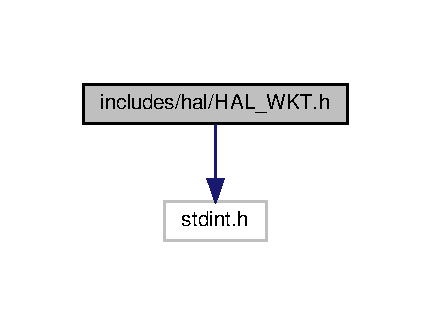
\includegraphics[width=207pt]{HAL__WKT_8h__incl}
\end{center}
\end{figure}
\subsection*{Enumeraciones}
\begin{DoxyCompactItemize}
\item 
\mbox{\Hypertarget{HAL__WKT_8h_afe3a7131eaa16754febfe27e0da02823}\label{HAL__WKT_8h_afe3a7131eaa16754febfe27e0da02823}} 
enum {\bfseries hal\+\_\+wkt\+\_\+clock\+\_\+source\+\_\+en} \{ {\bfseries H\+A\+L\+\_\+\+W\+K\+T\+\_\+\+C\+L\+O\+C\+K\+\_\+\+S\+O\+U\+R\+C\+E\+\_\+\+F\+R\+O\+\_\+\+D\+IV} = 0, 
{\bfseries H\+A\+L\+\_\+\+W\+K\+T\+\_\+\+C\+L\+O\+C\+K\+\_\+\+S\+O\+U\+R\+C\+E\+\_\+\+L\+O\+W\+\_\+\+P\+O\+W\+E\+R\+\_\+\+O\+SC}, 
{\bfseries H\+A\+L\+\_\+\+W\+K\+T\+\_\+\+C\+L\+O\+C\+K\+\_\+\+S\+O\+U\+R\+C\+E\+\_\+\+E\+X\+T\+E\+R\+N\+AL}
 \}
\end{DoxyCompactItemize}
\subsection*{Funciones}
\begin{DoxyCompactItemize}
\item 
void \hyperlink{HAL__WKT_8h_aeb732cadeaab8af681865670e8beab43}{hal\+\_\+wkt\+\_\+init} (hal\+\_\+wkt\+\_\+clock\+\_\+source\+\_\+en clock\+\_\+sel, uint32\+\_\+t ext\+\_\+clock\+\_\+value, void($\ast$callback)(void))
\begin{DoxyCompactList}\small\item\em Inicializar el W\+KT. \end{DoxyCompactList}\item 
\mbox{\Hypertarget{HAL__WKT_8h_a985343b8388f0830ebc106d298520d49}\label{HAL__WKT_8h_a985343b8388f0830ebc106d298520d49}} 
void {\bfseries hal\+\_\+wkt\+\_\+select\+\_\+clock\+\_\+source} (hal\+\_\+wkt\+\_\+clock\+\_\+source\+\_\+en clock\+\_\+sel, uint32\+\_\+t ext\+\_\+clock\+\_\+value)
\item 
void \hyperlink{HAL__WKT_8h_a83ba94b350eac43185f64f92e6a2ceab}{hal\+\_\+wkt\+\_\+register\+\_\+callback} (void($\ast$new\+\_\+callback)(void))
\begin{DoxyCompactList}\small\item\em Registrar un callback para la interrupcion del W\+KT. \end{DoxyCompactList}\item 
\mbox{\Hypertarget{HAL__WKT_8h_ab12f0980a1cf6c8338ea5df990ec2d13}\label{HAL__WKT_8h_ab12f0980a1cf6c8338ea5df990ec2d13}} 
void {\bfseries hal\+\_\+wkt\+\_\+start\+\_\+count} (uint32\+\_\+t time\+\_\+useg)
\item 
\mbox{\Hypertarget{HAL__WKT_8h_a1c617a5813b80a65229c86f810ae0c3b}\label{HAL__WKT_8h_a1c617a5813b80a65229c86f810ae0c3b}} 
void {\bfseries hal\+\_\+wkt\+\_\+start\+\_\+count\+\_\+with\+\_\+value} (uint32\+\_\+t value)
\end{DoxyCompactItemize}


\subsection{Descripción detallada}
Declaraciones a nivel de aplicacion del periferico W\+KT (L\+P\+C845) 

\begin{DoxyAuthor}{Autor}
Augusto Santini 
\end{DoxyAuthor}
\begin{DoxyDate}{Fecha}
3/2020 
\end{DoxyDate}
\begin{DoxyVersion}{Versión}
1.\+0 
\end{DoxyVersion}


\subsection{Documentación de las funciones}
\mbox{\Hypertarget{HAL__WKT_8h_aeb732cadeaab8af681865670e8beab43}\label{HAL__WKT_8h_aeb732cadeaab8af681865670e8beab43}} 
\index{H\+A\+L\+\_\+\+W\+K\+T.\+h@{H\+A\+L\+\_\+\+W\+K\+T.\+h}!hal\+\_\+wkt\+\_\+init@{hal\+\_\+wkt\+\_\+init}}
\index{hal\+\_\+wkt\+\_\+init@{hal\+\_\+wkt\+\_\+init}!H\+A\+L\+\_\+\+W\+K\+T.\+h@{H\+A\+L\+\_\+\+W\+K\+T.\+h}}
\subsubsection{\texorpdfstring{hal\+\_\+wkt\+\_\+init()}{hal\_wkt\_init()}}
{\footnotesize\ttfamily void hal\+\_\+wkt\+\_\+init (\begin{DoxyParamCaption}\item[{hal\+\_\+wkt\+\_\+clock\+\_\+source\+\_\+en}]{clock\+\_\+sel,  }\item[{uint32\+\_\+t}]{ext\+\_\+clock\+\_\+value,  }\item[{void($\ast$)(void)}]{callback }\end{DoxyParamCaption})}



Inicializar el W\+KT. 


\begin{DoxyParams}[1]{Parámetros}
\mbox{\tt in}  & {\em clock\+\_\+sel} & Seleccion de clock deseada para el W\+KT \\
\hline
\mbox{\tt in}  & {\em ext\+\_\+clock\+\_\+value} & Valor de clock externo (si la seleccion es interna, no importa este parametro) \\
\hline
\mbox{\tt in}  & {\em callback} & Callback a ejecutar en la interrupcion del W\+KT \\
\hline
\end{DoxyParams}
\mbox{\Hypertarget{HAL__WKT_8h_a83ba94b350eac43185f64f92e6a2ceab}\label{HAL__WKT_8h_a83ba94b350eac43185f64f92e6a2ceab}} 
\index{H\+A\+L\+\_\+\+W\+K\+T.\+h@{H\+A\+L\+\_\+\+W\+K\+T.\+h}!hal\+\_\+wkt\+\_\+register\+\_\+callback@{hal\+\_\+wkt\+\_\+register\+\_\+callback}}
\index{hal\+\_\+wkt\+\_\+register\+\_\+callback@{hal\+\_\+wkt\+\_\+register\+\_\+callback}!H\+A\+L\+\_\+\+W\+K\+T.\+h@{H\+A\+L\+\_\+\+W\+K\+T.\+h}}
\subsubsection{\texorpdfstring{hal\+\_\+wkt\+\_\+register\+\_\+callback()}{hal\_wkt\_register\_callback()}}
{\footnotesize\ttfamily void hal\+\_\+wkt\+\_\+register\+\_\+callback (\begin{DoxyParamCaption}\item[{void($\ast$)(void)}]{new\+\_\+callback }\end{DoxyParamCaption})}



Registrar un callback para la interrupcion del W\+KT. 


\begin{DoxyParams}[1]{Parámetros}
\mbox{\tt in}  & {\em new\+\_\+callback} & Nuevo callback para la interrupcion del W\+KT \\
\hline
\end{DoxyParams}

\chapter{Documentación de ejemplos}
\hypertarget{Ejemplo_ADC_8c-example}{}\doxysection{Ejemplo\+\_\+\+A\+D\+C.\+c}
Ejemplo sobre la utilización del {\itshape A\+D\+C.\+El} programa utiliza el clock por default con el que comienza el microcontrolador, es decir, el {\itshape Free Running Oscillator} funcionando a $ 12MHz $.

El periférico será configurado con las siguientes características\+:
\begin{DoxyItemize}
\item Funcionamiento {\bfseries{sincrónico}} 
\item Frecuencia de muestreo de $ 1Mhz $
\item Modo bajo consumo inhabilitado
\end{DoxyItemize}

La secuencia A es configurada para generar conversiones en los canales 0 y 8\+:
\begin{DoxyItemize}
\item El canal 0 está conectado al preset propio del stick de desarrollo (Puerto 0 pin 7)
\item El canal 8 está ubicado en el pin número 3 (Puerto 0 pin 18) y se le puede conectar un preset externo entre V\+DD y G\+ND.
\end{DoxyItemize}Además, la secuencia tendrá la siguiente configuración\+:
\begin{DoxyItemize}
\item Trigger\+: Únicamente se disparan conversiones por software
\item Bypass sincronismo\+: Sí
\item Modo de interrupción\+: Cuando termina la secuencia completa
\item Burst\+: Inhabilitado
\item Un trigger dispara\+: Una conversión de secuencia completa
\item Secuencia A como baja prioridad\+: No
\end{DoxyItemize}

Una vez inicializado el periférico, se configura el periférico {\itshape Systick} para interrumpir cada $ 1mseg $ y mediante su manejador se lleva la cuenta de los milisegundos transcurridos. Una vez transcurridos $ 1000mseg $, se dispara una conversión de {\itshape A\+DC}, y sus resultados se guardan en dos variables globales.

Ubicando un {\itshape breakpoint} adecuadamente, se pueden leer los resultados de las conversiones ya ubicadas en las variables globales.


\begin{DoxyCodeInclude}{0}
\DoxyCodeLine{\textcolor{comment}{/**}}
\DoxyCodeLine{\textcolor{comment}{ * @file Ejemplo\_ADC.c}}
\DoxyCodeLine{\textcolor{comment}{ * @brief Ejemplo de utilización del \(\backslash\)e ADC con la librería (capa de aplicación)}}
\DoxyCodeLine{\textcolor{comment}{ *}}
\DoxyCodeLine{\textcolor{comment}{ * El programa utiliza el clock por default con el que comienza el microcontrolador, es decir, el <em>Free Running}}
\DoxyCodeLine{\textcolor{comment}{ * Oscillator</em> funcionando a \(\backslash\)f\$ 12MHz \(\backslash\)f\$.}}
\DoxyCodeLine{\textcolor{comment}{ *}}
\DoxyCodeLine{\textcolor{comment}{ * El periférico será configurado con las siguientes características:}}
\DoxyCodeLine{\textcolor{comment}{ *  -\/ Funcionamiento \(\backslash\)b sincrónico}}
\DoxyCodeLine{\textcolor{comment}{ *  -\/ Frecuencia de muestreo de \(\backslash\)f\$ 1Mhz \(\backslash\)f\$}}
\DoxyCodeLine{\textcolor{comment}{ *  -\/ Modo bajo consumo inhabilitado}}
\DoxyCodeLine{\textcolor{comment}{ *  .}}
\DoxyCodeLine{\textcolor{comment}{ *}}
\DoxyCodeLine{\textcolor{comment}{ * La secuencia A es configurada para generar conversiones en los canales 0 y 8:}}
\DoxyCodeLine{\textcolor{comment}{ *  -\/ El canal 0 está conectado al preset propio del stick de desarrollo (Puerto 0 pin 7)}}
\DoxyCodeLine{\textcolor{comment}{ *  -\/ El canal 8 está ubicado en el pin número 3 (Puerto 0 pin 18) y se le puede conectar un preset externo entre}}
\DoxyCodeLine{\textcolor{comment}{ *   VDD y GND.}}
\DoxyCodeLine{\textcolor{comment}{ *  .}}
\DoxyCodeLine{\textcolor{comment}{ *}}
\DoxyCodeLine{\textcolor{comment}{ * Además, la secuencia tendrá la siguiente configuración:}}
\DoxyCodeLine{\textcolor{comment}{ *  -\/ Trigger: Únicamente se disparan conversiones por software}}
\DoxyCodeLine{\textcolor{comment}{ *  -\/ Bypass sincronismo: Sí}}
\DoxyCodeLine{\textcolor{comment}{ *  -\/ Modo de interrupción: Cuando termina la secuencia completa}}
\DoxyCodeLine{\textcolor{comment}{ *  -\/ Burst: Inhabilitado}}
\DoxyCodeLine{\textcolor{comment}{ *  -\/ Un trigger dispara: Una conversión de secuencia completa}}
\DoxyCodeLine{\textcolor{comment}{ *  -\/ Secuencia A como baja prioridad: No}}
\DoxyCodeLine{\textcolor{comment}{ *}}
\DoxyCodeLine{\textcolor{comment}{ * Una vez inicializado el periférico, se configura el periférico \(\backslash\)e Systick para interrumpir cada \(\backslash\)f\$ 1mseg \(\backslash\)f\$}}
\DoxyCodeLine{\textcolor{comment}{ * y mediante su manejador se lleva la cuenta de los milisegundos transcurridos. Una vez transcurridos}}
\DoxyCodeLine{\textcolor{comment}{ * \(\backslash\)f\$ 1000mseg \(\backslash\)f\$, se dispara una conversión de \(\backslash\)e ADC, y sus resultados se guardan en dos variables globales.}}
\DoxyCodeLine{\textcolor{comment}{ *}}
\DoxyCodeLine{\textcolor{comment}{ * Ubicando un \(\backslash\)e breakpoint adecuadamente, se pueden leer los resultados de las conversiones ya ubicadas en}}
\DoxyCodeLine{\textcolor{comment}{ * las variables globales.}}
\DoxyCodeLine{\textcolor{comment}{ *}}
\DoxyCodeLine{\textcolor{comment}{ * @author Augusto Santini}}
\DoxyCodeLine{\textcolor{comment}{ * @date 4/2020}}
\DoxyCodeLine{\textcolor{comment}{ */}}
\DoxyCodeLine{}
\DoxyCodeLine{\textcolor{preprocessor}{\#include <cr\_section\_macros.h>}}
\DoxyCodeLine{\textcolor{preprocessor}{\#include <stddef.h>}}
\DoxyCodeLine{\textcolor{preprocessor}{\#include <\mbox{\hyperlink{HAL__ADC_8h}{HAL\_ADC.h}}>}}
\DoxyCodeLine{\textcolor{preprocessor}{\#include <\mbox{\hyperlink{HAL__SYSTICK_8h}{HAL\_SYSTICK.h}}>}}
\DoxyCodeLine{}
\DoxyCodeLine{\textcolor{comment}{/* Máscara de configuración de canales habilitados para la secuencia a configurar */}}
\DoxyCodeLine{\textcolor{preprocessor}{\#define     ADC\_CHANNELS                ((1 << 0) | (1 << 8))}}
\DoxyCodeLine{}
\DoxyCodeLine{\textcolor{comment}{/* Macro para definir el tiempo de interrupción del \(\backslash\)e Systick en \(\backslash\)b microsegundos */}}
\DoxyCodeLine{\textcolor{preprocessor}{\#define     TICK\_TIME\_USEG              (1000)}}
\DoxyCodeLine{}
\DoxyCodeLine{\textcolor{comment}{/* Frecuencia de muestreo a utilizar por el ADC */}}
\DoxyCodeLine{\textcolor{preprocessor}{\#define     ADC\_SAMPLE\_FREQ             (1000000)}}
\DoxyCodeLine{\textcolor{comment}{}}
\DoxyCodeLine{\textcolor{comment}{/** Secuencia a utilizar en el ADC */}}
\DoxyCodeLine{\textcolor{preprocessor}{\#define     ADC\_SEQUENCE                (HAL\_ADC\_SEQUENCE\_SEL\_A)}}
\DoxyCodeLine{}
\DoxyCodeLine{\textcolor{comment}{/* Tiempo de disparo de conversiones de \(\backslash\)e ADC en \(\backslash\)b milisegundos */}}
\DoxyCodeLine{\textcolor{preprocessor}{\#define     ADC\_CONVERSION\_TIME\_MSEG    (1000)}}
\DoxyCodeLine{}
\DoxyCodeLine{\textcolor{keyword}{static} \textcolor{keywordtype}{void} adc\_callback(\textcolor{keywordtype}{void});}
\DoxyCodeLine{}
\DoxyCodeLine{\textcolor{keyword}{static} \textcolor{keywordtype}{void} systick\_callback(\textcolor{keywordtype}{void});}
\DoxyCodeLine{}
\DoxyCodeLine{\textcolor{keyword}{static} uint8\_t flag\_secuencia\_adc\_completada = 0; \textcolor{comment}{/* Flag para indicar finalización de secuencia de conversión de \(\backslash\)e ADC */}}
\DoxyCodeLine{}
\DoxyCodeLine{\textcolor{comment}{/*}}
\DoxyCodeLine{\textcolor{comment}{ * Variables para guardar los resultados de la secuencia de conversión}}
\DoxyCodeLine{\textcolor{comment}{ */}}
\DoxyCodeLine{\textcolor{keyword}{static} \mbox{\hyperlink{group__ADC_structhal__adc__sequence__result__t}{hal\_adc\_sequence\_result\_t}} resultados\_conversion\_adc[2];}
\DoxyCodeLine{}
\DoxyCodeLine{\textcolor{comment}{/* Configuración de la secuencia. Como no va a cambiar es declarada \(\backslash\)e const */}}
\DoxyCodeLine{\textcolor{keyword}{static} \textcolor{keyword}{const} \mbox{\hyperlink{group__ADC_structhal__adc__sequence__config__t}{hal\_adc\_sequence\_config\_t}} adc\_config =}
\DoxyCodeLine{\{}
\DoxyCodeLine{    .\mbox{\hyperlink{group__ADC_acebe3f0fdc69a72787ddd6b19870641b}{channels}} = ADC\_CHANNELS,}
\DoxyCodeLine{    .trigger = \mbox{\hyperlink{group__ADC_gga67fe859b54301579f1b1daef874514caaaf722f012bd0aa063b595333f9012a20}{HAL\_ADC\_TRIGGER\_SEL\_NONE}},}
\DoxyCodeLine{    .trigger\_pol = \mbox{\hyperlink{group__ADC_gga4c5aa9e0991c432640845d2aedb971b2a007c22a34504d8557d98704becf95dc8}{HAL\_ADC\_TRIGGER\_POL\_SEL\_NEGATIVE\_EDGE}},}
\DoxyCodeLine{    .sync\_bypass = \mbox{\hyperlink{group__ADC_gga8aa0efd767a9edc5a80b80c4061e0904a1cbf7646bbe7c32e3e21663fc5952d77}{HAL\_ADC\_SYNC\_SEL\_BYPASS\_SYNC}},}
\DoxyCodeLine{    .mode = \mbox{\hyperlink{group__ADC_ggaf4981172881d597ede49249ba04fcafeae73eff6d5c4ef7297d31a28e4a76e149}{HAL\_ADC\_INTERRUPT\_MODE\_EOS}},}
\DoxyCodeLine{    .burst = 0,}
\DoxyCodeLine{    .single\_step = 0,}
\DoxyCodeLine{    .low\_priority = 0,}
\DoxyCodeLine{    .callback = adc\_callback}
\DoxyCodeLine{\};}
\DoxyCodeLine{}
\DoxyCodeLine{\textcolor{comment}{/*}}
\DoxyCodeLine{\textcolor{comment}{ * @brief Punto de entrada del programa}}
\DoxyCodeLine{\textcolor{comment}{ * @return Nunca deberia terminar esta función}}
\DoxyCodeLine{\textcolor{comment}{ */}}
\DoxyCodeLine{\textcolor{keywordtype}{int} main(\textcolor{keywordtype}{void})}
\DoxyCodeLine{\{}
\DoxyCodeLine{    \textcolor{comment}{// Inicialización del periférico en modo SINCRÓNICO}}
\DoxyCodeLine{    \mbox{\hyperlink{group__ADC_ga952626700075b275e7766c0095e4ec36}{hal\_adc\_init\_sync\_mode}}(ADC\_SAMPLE\_FREQ, \mbox{\hyperlink{group__ADC_ggaf1570443ca3570a7ae83b90307bbeccaaf92172fb70ce285c23631cb025b3cd52}{HAL\_ADC\_LOW\_POWER\_MODE\_DISABLED}});}
\DoxyCodeLine{}
\DoxyCodeLine{    \textcolor{comment}{// Configuración de la secuencia a utilizar}}
\DoxyCodeLine{    \mbox{\hyperlink{group__ADC_gadcef726eaa85af74ade96c14f9a48feb}{hal\_adc\_config\_sequence}}(ADC\_SEQUENCE, \&adc\_config);}
\DoxyCodeLine{}
\DoxyCodeLine{    \textcolor{comment}{// Inicialización del \(\backslash\)e Systick con el tiempo de tick adecuado}}
\DoxyCodeLine{    \mbox{\hyperlink{HAL__SYSTICK_8h_a29eb17e59d26a3f1a1f9184154964f36}{hal\_systick\_init}}(TICK\_TIME\_USEG, systick\_callback);}
\DoxyCodeLine{}
\DoxyCodeLine{    \textcolor{keywordflow}{while}(1)}
\DoxyCodeLine{    \{}
\DoxyCodeLine{        \textcolor{keywordflow}{if}(flag\_secuencia\_adc\_completada == 1) \textcolor{comment}{// Esto o hacer "if(flag\_secuencia\_adc\_completada)" es indistinto}}
\DoxyCodeLine{        \{}
\DoxyCodeLine{            uint32\_t variable\_auxiliar;}
\DoxyCodeLine{}
\DoxyCodeLine{            flag\_secuencia\_adc\_completada = 0;}
\DoxyCodeLine{}
\DoxyCodeLine{            (void) variable\_auxiliar; \textcolor{comment}{// Esta línea es ideal para colocar el breakpoint!}}
\DoxyCodeLine{        \}}
\DoxyCodeLine{    \}}
\DoxyCodeLine{}
\DoxyCodeLine{    \textcolor{keywordflow}{return} 0;}
\DoxyCodeLine{\}}
\DoxyCodeLine{}
\DoxyCodeLine{\textcolor{comment}{/*}}
\DoxyCodeLine{\textcolor{comment}{ * @brief Callback a ejecutar en cada tick del \(\backslash\)e Systick}}
\DoxyCodeLine{\textcolor{comment}{ */}}
\DoxyCodeLine{\textcolor{keyword}{static} \textcolor{keywordtype}{void} systick\_callback(\textcolor{keywordtype}{void})}
\DoxyCodeLine{\{}
\DoxyCodeLine{    \textcolor{keyword}{static} uint32\_t contador\_disparo\_adc = 0;}
\DoxyCodeLine{}
\DoxyCodeLine{    \textcolor{comment}{// Conteo con valor límite}}
\DoxyCodeLine{    contador\_disparo\_adc = (contador\_disparo\_adc + 1) \% ADC\_CONVERSION\_TIME\_MSEG;}
\DoxyCodeLine{}
\DoxyCodeLine{    \textcolor{keywordflow}{if}(contador\_disparo\_adc == 0) \textcolor{comment}{// Esto o hacer "if(!contador\_disparo\_adc)" es indistinto}}
\DoxyCodeLine{    \{}
\DoxyCodeLine{        \mbox{\hyperlink{group__ADC_ga154950a81b5f589fde0139178ab1dcf3}{hal\_adc\_start\_sequence}}(ADC\_SEQUENCE);}
\DoxyCodeLine{    \}}
\DoxyCodeLine{\}}
\DoxyCodeLine{}
\DoxyCodeLine{\textcolor{comment}{/*}}
\DoxyCodeLine{\textcolor{comment}{ * @brief Callback a ejecutar en cada finalización de conversión de \(\backslash\)b secuencia de \(\backslash\)e ADC}}
\DoxyCodeLine{\textcolor{comment}{ */}}
\DoxyCodeLine{\textcolor{keyword}{static} \textcolor{keywordtype}{void} adc\_callback(\textcolor{keywordtype}{void})}
\DoxyCodeLine{\{}
\DoxyCodeLine{    \textcolor{comment}{// Obtención de resultados de conversión}}
\DoxyCodeLine{    \mbox{\hyperlink{group__ADC_gaf58fbae95e4083bddf74495df7709674}{hal\_adc\_get\_sequence\_result}}(ADC\_SEQUENCE, resultados\_conversion\_adc);}
\DoxyCodeLine{}
\DoxyCodeLine{    flag\_secuencia\_adc\_completada = 1;}
\DoxyCodeLine{\}}
\end{DoxyCodeInclude}
 
%--- End generated contents ---

% Index
\backmatter
\newpage
\phantomsection
\clearemptydoublepage
\addcontentsline{toc}{chapter}{Índice}
\printindex

\end{document}
